\documentclass[10pt, letterpaper]{article}

% Inhaltsverzeichnis für Pakettypen (nur für Übersicht im Header, wird nicht im Dokument angezeigt)
% 1. Seitenlayout und Ränder
% 2. Sprache und Zeichensatz
% 3. Mathematik und Theorem-Umgebungen
% 4. Eigene Makros
% 5. Diagramme und Grafiken
% 6. Tabellen und Aufzählungen
% 7. Inhaltsverzeichnis
% 8. Abschnittsüberschriften
% 9. Abstrakt-Umgebung
% 10. Todos/Notizen
% 11. Rahmen/Box-Umgebungen
% 12. Python-Integration
% 13. Literaturverwaltung
% 14. Hyperlinks
% 15. Absatzeinstellungen
% 16. Umgebungen
% 17  Graphik
% 00. Titel und Autor

% --- 1. Seitenlayout und Ränder ---
\usepackage[margin=3cm]{geometry}

% --- 2. Sprache und Zeichensatz ---
\usepackage[english]{babel}
\usepackage[T1]{fontenc}
\usepackage[utf8]{inputenc}

% --- 3. Mathematik und Theorem-Umgebungen ---
\usepackage{amsmath, amssymb, amsthm}
\usepackage{mathrsfs}
\DeclareMathOperator{\WF}{WF}

% --- 4. Eigene Makros ---
\usepackage{xcolor}
\newcommand{\SKP}{\langle\cdot,\cdot\rangle}
\newcommand{\R}{\mathbb{R}}
\newcommand{\N}{\mathbb{N}}
\newcommand{\Q}{\mathbb{Q}}
\newcommand{\Z}{\mathbb{Z}}
\newcommand{\C}{\mathbb{C}}
\newcommand{\entwurf}[1]{\textcolor{red}{#1}}

% --- 5. Diagramme und Grafiken ---
\usepackage{graphicx}
\usepackage{tikz}
\usetikzlibrary{decorations.pathreplacing, arrows.meta, positioning}
\usepackage{tikz-cd}

% --- 6. Tabellen und Aufzählungen ---
\usepackage{enumitem}
\setlist[itemize]{left=0.5cm}

\newenvironment{romanenum}[1][]
  {%
    \ifx&#1&
    \else
      \textbf{#1}\quad
    \fi
    \begin{enumerate}[label=\roman*)]
  }
  {%
    \end{enumerate}%
  }

% --- 7. Inhaltsverzeichnis ---
\usepackage{tocloft}
\renewcommand{\cftsecfont}{\footnotesize}
\renewcommand{\cftsubsecfont}{\footnotesize}
\renewcommand{\cftsubsubsecfont}{\footnotesize}
\renewcommand{\cftsecpagefont}{\footnotesize}
\renewcommand{\cftsubsecpagefont}{\footnotesize}
\renewcommand{\cftsubsubsecpagefont}{\footnotesize}
\usepackage{etoc}

% --- 8. Abschnittsüberschriften ---
\usepackage{titlesec}
\titleformat{\section}{\normalfont\large\bfseries}{\thesection}{1em}{}
\titleformat{\subsection}{\normalfont\normalsize\bfseries}{\thesubsection}{0.5em}{}
\titleformat{\subsubsection}{\normalfont\normalsize\bfseries}{\thesubsubsection}{0.5em}{}
\setcounter{secnumdepth}{4}

% --- 9. Abstrakt-Umgebung ---
\usepackage{changepage}
\renewenvironment{abstract}
  {
    \begin{adjustwidth}{1.5cm}{1.5cm}
    \small
    \textsc{Abstract. –}%
  }
  {
    \end{adjustwidth}
  }

% --- 10. Todos/Notizen ---
\usepackage{todonotes}

% --- 11. Rahmen/Box-Umgebungen ---
\usepackage{mdframed}
\usepackage{tcolorbox}
\colorlet{shadecolor}{gray!25}

\newenvironment{customTheorem}
  {\vspace{10pt}%
   \begin{mdframed}[
     backgroundcolor=gray!20,
     linewidth=0pt,
     innertopmargin=10pt,
     innerbottommargin=10pt,
     skipabove=\dimexpr\topsep+\ht\strutbox\relax,
     skipbelow=\topsep,
   ]}
  {\end{mdframed}
   \vspace{10pt}%
  }

% --- 12. Python-Integration ---
% (Deaktiviert in dieser Version, aktiviere bei Bedarf)
% \usepackage{pythontex}
% \usepackage[makestderr]{pythontex}

% --- 13. Literaturverwaltung ---
\usepackage{csquotes}
\usepackage[backend=biber, style=alphabetic, citestyle=alphabetic]{biblatex}
\addbibresource{bibliography.bib}

% --- 14. Hyperlinks ---
\usepackage{hyperref}
\hypersetup{
  colorlinks   = true,
  urlcolor     = blue,
  linkcolor    = blue,
  citecolor    = blue,
  frenchlinks  = true
}

% --- 15. Absatzeinstellungen ---
\usepackage[parfill]{parskip}
\sloppy

% --- 16. Umgebungen ---
\usepackage{thmtools}

\newcommand{\CustomHeading}[3]{%
  \par\medskip\noindent%
  \textbf{#1 #2} \textnormal{(#3)}.\enskip%
}

\newenvironment{DEF}[2]{\begin{unitbox}\CustomHeading{Definition}{#1}{#2}}{\end{unitbox}}
\newenvironment{PROP}[2]{\begin{unitbox}\CustomHeading{Proposition}{#1}{#2}}{\end{unitbox}}
\newenvironment{THEO}[2]{\begin{unitbox}\CustomHeading{Theorem}{#1}{#2}}{\end{unitbox}}
\newenvironment{LEM}[2]{\begin{unitbox}\CustomHeading{Lemma}{#1}{#2}}{\end{unitbox}}
\newenvironment{KORO}[2]{\begin{unitbox}\CustomHeading{Corollar}{#1}{#2}}{\end{unitbox}}
\newenvironment{REM}[2]{\begin{unitbox}\CustomHeading{Remark}{#1}{#2}}{\end{unitbox}}
\newenvironment{EXA}[2]{\begin{unitbox}\CustomHeading{Example}{#1}{#2}}{\end{unitbox}}
\newenvironment{STUD}[2]{\begin{unitbox}\CustomHeading{Study}{#1}{#2}}{\end{unitbox}}
\newenvironment{CONC}[2]{\begin{unitbox}\CustomHeading{Concept}{#1}{#2}}{\end{unitbox}}

\newenvironment{PROOF}
  {\begin{proof}}%
{\end{proof}}

% --- Unit Umgebung für Source-Inhalte ---
\usepackage{mdframed}
\newmdenv[
  linewidth=1pt,
  topline=false,
  bottomline=false,
  rightline=false,
  leftmargin=0cm,
  rightmargin=0cm,
  skipabove=10pt,
  skipbelow=10pt,
  innertopmargin=0.5\baselineskip,
  innerbottommargin=0.5\baselineskip,
  backgroundcolor=gray!10,
  linecolor=gray
]{unitbox}

\newenvironment{unit}[1]
  {\begin{unitbox}\textbf{Unit #1}\par\smallskip}
  {\end{unitbox}}

% --- 17. Graphik ---
\usepackage{graphicx}
\graphicspath{ {./images/} }
\usepackage[export]{adjustbox}

% --- 00. Titel und Autor ---
\title{Mein Titel}
\author{Tim Jaschik}
\date{\today}

\begin{document}

\maketitle
\rule{\textwidth}{0.5pt}
\begin{abstract}
Kurze Beschreibung …
\end{abstract}
\rule{\textwidth}{0.5pt}
\vspace{0.5cm}

\tableofcontents

\pagebreak




\section{Summary}
The notion of symmetry, i.e., the invariance of a theory under certain transformations of its degrees of freedom, plays an important, if not the most important, role in the mathematical formulation of the laws of Nature.

The notion of symmetry is already known from lecture courses on "Mechanics". According to Noether's theorem, the invariance of the action under coordinate transformations

$$
\begin{aligned}
t & \longrightarrow t^{\prime}(t) \\
\vec{q}(t) & \longrightarrow \vec{q}^{\prime}(\vec{q}(t), t)
\end{aligned}
$$

leads to integrals of motion, i.e., to conservation laws. A transformation which leaves the action invariant is called symmetry transformation or symmetry.

As we shall see in this lecture course, the notion of symmetry can be applied to quantum-mechanical systems, too. Also in this case, we will be lead to integrals of motion. However, we will not derive them via the invariance of the action, as in Noether's theorem, but we will directly investigate the behavior of Schrödinger's equation under symmetry transformations (Chapter 2). To understand the mathematical structure of symmetry transformations in quantum mechanics, we will give a short introduction to group theory (Chapter 3).

We will see that symmetries of a theory are not restricted to the invariance under coordinate transformations. At least of equal importance is the class of so-called internal symmetries, i.e., transformations which are not related to the space-time coordinates of the system. Of fundamental importance for physics is the group of unitary transformations in three dimensions, $S U(3)$ (Chapter 4), and its applications in the theory of strong interactions in particle physics (Chapter 5).

We will conclude this lecture course by a discussion of the Poincaré group, which is of eminent importance in relativistic quantum field theory (Chapter 6), because all theories of Nature (which are well-established up to now) are formulated to respect this symmetry.

\section{Symmetries in Quantum Mechanics}
\subsection{Space translations}
Consider the Hilbert-space state $|\psi\rangle$. We can assign a coordinate-space wave function to this state according to

$$
|\psi\rangle \longrightarrow \psi(\vec{r}) \equiv\langle\vec{r} \mid \psi\rangle .
$$

Let us now consider a translation in space

$$
\vec{r} \longrightarrow \vec{r}^{\prime}=\vec{r}+\vec{a},
$$

where $\vec{a}=\overrightarrow{\text { const. }}$. If we demand that physics is invariant under such space translations, i.e., that the space translation 2.1 is a symmetry transformation, then we must have for the transformed wave function

$$
\psi^{\prime}\left(\vec{r}^{\prime}\right) \equiv \psi(\vec{r}),
$$

i.e., the transformed wave function $\psi^{\prime}$ at the transformed position $\vec{r}^{\prime}$ has to be equal to the original wave function $\psi$ at the original position $\vec{r}$. Using Eq. (2.1) we may write Eq. (2.2) as follows

$$
\psi^{\prime}(\vec{r}+\vec{a})=\psi(\vec{r}) \quad \text { or } \quad \psi^{\prime}(\vec{r})=\psi(\vec{r}-\vec{a})
$$

Using the so-called spatial translation operator $\hat{U}_{r}(\vec{a})$ the last equation can be expressed as follows

$$
\psi^{\prime}(\vec{r})=\hat{U}_{r}(\vec{a}) \psi(\vec{r})
$$

If a space translation is a symmetry transformation, it cannot influence the probability with which a quantum-mechanical state occurs. According to the conservation of probability we therefore have

$$
\begin{aligned}
\left\langle\psi^{\prime} \mid \psi^{\prime}\right\rangle & =\int \mathrm{d}^{3} \vec{r}\left\langle\psi^{\prime} \mid \vec{r}\right\rangle\left\langle\vec{r} \mid \psi^{\prime}\right\rangle=\int \mathrm{d}^{3} \vec{r} \psi^{\prime *}(\vec{r}) \psi^{\prime}(\vec{r})=\int \mathrm{d}^{3} \vec{r}\left[\hat{U}_{r}(\vec{a}) \psi(\vec{r})\right]^{*} \hat{U}_{r}(\vec{a}) \psi(\vec{r}) \\
& =\int \mathrm{d}^{3} \vec{r} \psi^{*}(\vec{r}) \hat{U}_{r}^{\dagger}(\vec{a}) \hat{U}_{r}(\vec{a}) \psi(\vec{r}) \equiv \int \mathrm{d}^{3} \vec{r} \psi^{*}(\vec{r}) \psi(\vec{r})=\langle\psi \mid \psi\rangle
\end{aligned}
$$

This means that $\hat{U}_{\vec{r}}(\vec{a})$ must be a unitary operator,

$$
\hat{U}_{r}^{\dagger}(\vec{a}) \hat{U}_{r}(\vec{a}) \equiv \mathbf{1} \quad \Longleftrightarrow \quad \hat{U}_{r}^{\dagger}(\vec{a})=\hat{U}_{r}^{-1}(\vec{a})
$$

Let us now explicitly determine this operator. Without restriction of generality we consider a translation in $x$-direction, $\vec{a}=(a, 0,0)^{T}$, and expand the right-hand side of Eq.\\
(2.3) in terms of a Taylor series around the point $\vec{r}$,

$$
\begin{aligned}
\psi(\vec{r}-\vec{a}) & =\psi(\vec{r})-a \frac{\partial}{\partial x} \psi(\vec{r})+\frac{1}{2!} a^{2} \frac{\partial^{2}}{\partial x^{2}} \psi(\vec{r})-\frac{1}{3!} a^{3} \frac{\partial^{3}}{\partial x^{3}} \psi(\vec{r})+\ldots \\
& =\sum_{n=0}^{\infty} \frac{(-a)^{n}}{n!} \frac{\partial^{n}}{\partial x^{n}} \psi(\vec{r}) \equiv \exp \left(-a \frac{\partial}{\partial x}\right) \psi(\vec{r}) \\
& =\exp \left(-\frac{i}{\hbar} a \hat{p}^{x}\right) \psi(\vec{r}) \equiv \exp \left(-\frac{i}{\hbar} \vec{a} \cdot \hat{\vec{p}}\right) \psi(\vec{r})
\end{aligned}
$$

where we have used the momentum operator $\hat{\vec{p}}=-i \hbar \vec{\nabla}$. Comparison with Eq. 2.4 yields

$$
\hat{U}_{r}(\vec{a}) \equiv \exp \left(-\frac{i}{\hbar} \vec{a} \cdot \hat{\vec{p}}\right)
$$

This form of the space-translation operator holds also for arbitrary vectors $\vec{a}$. The momentum operator $\hat{\vec{p}}$ is hermitean (since the momentum is a physical observable), $\hat{\vec{p}}^{\dagger} \equiv \hat{\vec{p}}$, and thus the unitarity $(2.6)$ of the space-translation operator $\hat{U}_{r}(\vec{a})$ is immediately obvious. On the one hand we have

$$
\hat{U}_{r}^{\dagger}(\vec{a})=\exp \left(+\frac{i}{\hbar} \vec{a} \cdot \hat{\vec{p}}^{\dagger}\right)=\exp \left[-\frac{i}{\hbar}(-\vec{a}) \cdot \hat{\vec{p}}\right]=\hat{U}_{r}(-\vec{a})
$$

where we used that $\vec{a} \in \mathbb{R}^{3}$. On the other hand, since a translation by $-\vec{a}$ reverses the translation by $+\vec{a}$,

$$
\hat{U}_{r}(-\vec{a}) \hat{U}_{r}(\vec{a}) \equiv \mathbf{1}
$$

one has

$$
\hat{U}_{r}^{\dagger}(\vec{a})=\hat{U}_{r}(-\vec{a})=\hat{U}_{r}^{-1}(\vec{a}), \quad \text { q.e.d. }
$$

If the space translation (2.1) is a symmetry transformation, the Hamilton operator has to be invariant, too,

$$
\hat{H} \longrightarrow \hat{H}^{\prime} \equiv \hat{H} \quad\left(\vec{r} \longrightarrow \vec{r}^{\prime}=\vec{r}+\vec{a}\right)
$$

The transformed wave function (2.2) obeys the (in general time-dependent) Schrödinger equation,

$$
i \hbar \frac{\partial}{\partial t} \psi^{\prime}(t, \vec{r})=\hat{H} \psi^{\prime}(t, \vec{r})
$$

If we insert Eq. (2.4) (a possible time dependence of the wave function does not influence this equation), we obtain

$$
i \hbar \frac{\partial}{\partial t} \hat{U}_{r}(\vec{a}) \psi(t, \vec{r}) \equiv \hat{U}_{r}(\vec{a}) i \hbar \frac{\partial}{\partial t} \psi(t, \vec{r})=\hat{H} \hat{U}_{r}(\vec{a}) \psi(t, \vec{r})
$$

since temporal and spatial derivatives commute with each other. Since the original wave function also fulfills the time-dependent Schrödinger equation,

$$
i \hbar \frac{\partial}{\partial t} \psi(t, \vec{r})=\hat{H} \psi(t, \vec{r})
$$

we can write Eq. (2.11) as

$$
\hat{U}_{r}(\vec{a}) \hat{H} \psi(t, \vec{r})=\hat{H} \hat{U}_{r}(\vec{a}) \psi(t, \vec{r}),
$$

or, since the wave function $\psi(t, \vec{r})$ was arbitrary,

$$
\hat{U}_{r}(\vec{a}) \hat{H}=\hat{H} \hat{U}_{r}(\vec{a}) \quad \Longleftrightarrow \quad\left[\hat{U}_{r}(\vec{a}), \hat{H}\right]=0,
$$

where we introduced the commutator of two operators $\hat{A}, \hat{B}$,

$$
[\hat{A}, \hat{B}] \equiv \hat{A} \hat{B}-\hat{B} \hat{A} .
$$

Thus, a space translation is a symmetry transformation, if the space-translation operator $\hat{U}_{r}(\vec{a})$ commutes with the Hamilton operator of the system.

This must also be valid for infinitesimal space translations, $|\vec{a}| \ll \hbar /|\langle\hat{\vec{p}}\rangle|$. For such one can expand the space-translation operator (2.7) in terms of a Taylor series,

$$
\hat{U}_{r}(\vec{a}) \simeq \mathbf{1}-\frac{i}{\hbar} \vec{a} \cdot \hat{\vec{p}},
$$

where we can neglect terms of order $O\left(a^{2}\right)$. Inserting this into Eq. (2.14) yields

$$
\left[\mathbf{1}-\frac{i}{\hbar} \vec{a} \cdot \hat{\vec{p}}, \hat{H}\right] \equiv \frac{i}{\hbar} \vec{a} \cdot[\hat{\vec{p}}, \hat{H}]=0 \quad \Longleftrightarrow \quad[\hat{\vec{p}}, \hat{H}]=0
$$

since the infinitesimal translation vector $\vec{a}$ was arbitrary. We conclude that, for systems invariant under space translations, the momentum operator commutes with the Hamilton operator. Then, however, the momentum is an integral of motion, i.e., we have momentum conservation, and one can find a system of eigenstates of $\hat{H}$ which are simultaneously eigenstates of $\hat{\vec{p}}$.

\subsection{Time translations}
We now consider translations in time,

$$
t \longrightarrow t^{\prime}=t+a,
$$

where $a=$ const.. We demand that physics remains invariant under such translations in time, i.e., the time translation (2.18) is a symmetry transformation. Then the transformed wave function must fulfill (we suppress a potential spatial dependence, since it does not play any role in the following)

$$
\psi^{\prime}\left(t^{\prime}\right)=\psi(t),
$$

i.e., the transformed wave function $\psi^{\prime}$ at the shifted time $t^{\prime}$ must be identical to the original wave function $\psi$ at the original time $t$. If we insert Eq. (2.18), we can write this in the following way,

$$
\psi^{\prime}(t+a)=\psi(t) \quad \Longleftrightarrow \quad \psi^{\prime}(t)=\psi(t-a) \equiv \hat{U}_{t}(a) \psi(t),
$$

where, in analogy to the preceding section, we have again expressed the effect of the time translation by an operator, the so-called time-translation operator $\hat{U}_{t}(a)$. In complete analogy to the derivation of the space-translation operator (2.7) we now obtain

$$
\hat{U}_{t}(a)=\exp \left(-a \frac{\partial}{\partial t}\right) \equiv \exp \left(\frac{i}{\hbar} a \hat{E}\right),
$$

with the energy operator $\hat{E} \equiv i \hbar \partial / \partial t$. The unitarity of the time-translation operator follows from the hermiticity of the energy operator, $\hat{E}^{\dagger} \equiv \hat{E}$ (energy eigenvalues are always real-valued), and from $a \in \mathbb{R}$.

Acting with the operator (2.21) on states which fulfill the time-dependent Schrödinger equation (2.12) yields the identity $\hat{E} \equiv \hat{H}$, such that we can also write the time-translation operator (2.21) as

$$
\hat{U}_{t}(a) \equiv \exp \left(\frac{i}{\hbar} \hat{H} a\right)
$$

Thus, it is identical to the time-evolution operator well-known from lectures on quantum mechanics, for Hamilton operators which do not explicitly depend on time. (Note that the time translation (2.18) affects a time evolution of the state $\psi(t)$ into the state $\psi(t-a)$, cf. Eq. 2.20 , i.e., backwards in time by an amount $-a$.)

Symmetry under time translations means that also the Hamilton operator remains invariant,

$$
\hat{H} \longrightarrow \hat{H}^{\prime} \equiv \hat{H} \quad\left(t \longrightarrow t^{\prime}=t+a\right)
$$

The time-translated state $\psi^{\prime}(t)$ of course fulfills the time-dependent Schrödinger equation

$$
\begin{aligned}
i \hbar \frac{\partial}{\partial t} \psi^{\prime}(t) & =\hat{H} \psi^{\prime}(t) \\
\Longleftrightarrow \quad i \hbar \frac{\partial}{\partial t} \hat{U}_{t}(a) \psi(t) & \equiv \hat{U}_{t}(a) i \hbar \frac{\partial}{\partial t} \psi(t)=\hat{U}_{t}(a) \hat{H} \psi(t)=\hat{H} \hat{U}_{t}(a) \psi(t)
\end{aligned}
$$

where we have used Eq. (2.20) and the original Schrödinger equation (2.12) for the state $\psi(t)$. Since this holds for an arbitrary wave function, we get

$$
\hat{U}_{t}(a) \hat{H}=\hat{H} \hat{U}_{t}(a) \Longleftrightarrow\left[\hat{U}_{t}(a), \hat{H}\right]=0
$$

in analogy to Eq. (2.14) for space translations. If the system is invariant under time translations, the time-translation operator commutes with the Hamilton operator.

Since this holds also for infinitesimal time translations, $|a| \ll \hbar /|\langle\hat{E}\rangle|$, after Taylorexpanding the time-translation operator 2.21 we obtain

$$
[\hat{E}, \hat{H}]=\left[i \hbar \frac{\partial}{\partial t}, \hat{H}\right]=0 \quad \Longleftrightarrow \quad \frac{\partial \hat{H}}{\partial t}=0
$$

i.e., the Hamilton operator must not depend explicitly on time. For systems which are invariant under time translations, the time-translation operator is thus identical to the time-evolution operator, cf. Eq. (2.22). The conserved quantity associated with this symmetry is the total energy of the system.

\subsection{Rotations}
Let us consider a rotation in space by an infinitesimal angle $\delta \vec{\phi}$ (around an axis defined by the direction of $\delta \vec{\phi}$ ),

$$
\vec{r} \longrightarrow \vec{r}^{\prime}=\vec{r}+\delta \vec{\phi} \times \vec{r} .
$$

We demand that this is a symmetry transformation, i.e.,

$$
\psi^{\prime}\left(\vec{r}^{\prime}\right)=\psi(\vec{r}) \quad \Longleftrightarrow \quad \psi^{\prime}(\vec{r})=\psi(\vec{r}-\delta \vec{\phi} \times \vec{r}) .
$$

For infinitesimal rotation angles, $|\delta \vec{\phi}| \ll 1$ we may again expand the right-hand side in terms of a Taylor series, which we can truncate at order $O\left(\delta \phi^{2}\right)$,

$$
\begin{aligned}
\psi^{\prime}(\vec{r}) & =\psi(\vec{r})-(\delta \vec{\phi} \times \vec{r}) \cdot \vec{\nabla} \psi(\vec{r})+O\left(\delta \phi^{2}\right) \\
& \simeq \psi(\vec{r})-\delta \vec{\phi} \cdot(\vec{r} \times \vec{\nabla}) \psi(\vec{r}) \equiv\left[1-\frac{i}{\hbar} \delta \vec{\phi} \cdot(\vec{r} \times \hat{\vec{p}})\right] \psi(\vec{r}) \\
& =\left(11-\frac{i}{\hbar} \delta \vec{\phi} \cdot \hat{\vec{L}}\right) \psi(\vec{r}),
\end{aligned}
$$

where we have used the definitions of the triple product, of the momentum operator, $\hat{\vec{p}}=-i \hbar \vec{\nabla}$, and of the orbital angular-momentum operator, $\hat{\vec{L}}=\vec{r} \times \hat{\vec{p}}$. We again demand that the transformation (2.28) is affected by an operator,

$$
\psi^{\prime}(\vec{r})=\psi(\vec{r}-\delta \vec{\phi} \times \vec{r})=\hat{U}_{R}(\delta \vec{\phi}) \psi(\vec{r}) .
$$

A comparison with Eq. (2.29) shows that the infinitesimal rotation operator has the form

$$
\hat{U}_{R}(\delta \vec{\phi})=\mathbf{1}-\frac{i}{\hbar} \delta \vec{\phi} \cdot \hat{\vec{L}} .
$$

These are the first two terms of the Taylor expansion of the exponential function. The rotation operator for arbitrary (not necessarily infinitesimal) rotation angles is thus defined as

$$
\hat{U}_{R}(\vec{\phi}) \equiv \exp \left(-\frac{i}{\hbar} \vec{\phi} \cdot \hat{\vec{L}}\right) .
$$

The unitarity of the rotation operator follows from the hermiticity of the orbital angularmomentum operator, $\hat{\vec{L}}^{\dagger}=\hat{\vec{L}}$, and from $\vec{\phi} \in \mathbb{R}^{3}$.

For systems which are invariant under rotations the Hamilton operator must also remain invariant,

$$
\hat{H} \longrightarrow \hat{H}^{\prime}=\hat{H} \quad\left(\vec{r} \longrightarrow \vec{r}^{\prime}=\vec{r}+\vec{\phi} \times \vec{r}\right) .
$$

By the same arguments as in the two preceding sections one then shows that

$$
\left[\hat{U}_{R}(\vec{\phi}), \hat{H}\right]=0,
$$

i.e., the rotation operator commutes with the Hamilton operator. For infinitesimal rotations this is equivalent to

$$
[\overrightarrow{\vec{L}}, \hat{H}]=0 .
$$

This means that the orbital angular momentum is conserved and that one can find a common system of eigenstates of $\hat{H}, \hat{\vec{L}}^{2}$ and $\hat{L}^{z}$.

\section{Introduction to Group Theory}
Definition: A set

$$
G=\{a, b, c, \ldots\}
$$

is a group, if there exists an operation ("multiplication"), which combines elements $a, b \in G$,

$$
a \circ b
$$

with the following properties:\\
(i) Closure: $\forall a, b \in G$ also $a \circ b \in G$.

One says that $G$ is closed under the operation (multiplication) which combines group elements.\\
(ii) Identity element: $\exists e \in G$, such that $\forall a \in G$ it holds that $a \circ e=e \circ a=a$, i.e., a so-called identity element exists.\\
(iii) Inverse element: $\forall a \in G \exists a^{-1} \in G$, such that $a^{-1} \circ a=a \circ a^{-1}=e$, i.e., for each group element exists an inverse element.\\
(iv) Associativity: $\forall a, b, c \in G$ it holds that $(a \circ b) \circ c=a \circ(b \circ c)$, the so-called law of associativity of group multiplication.

The group multiplication is essential to the definition of the group, hence one also denotes the group by ( $G, \circ$ ), i.e., the set of elements $G$ which are combined by the group multiplication $\circ$.\\
Definition: A group ( $G, \circ$ ) is called abelian, if $\forall a, b \in G$ it holds that $a \circ b=b \circ a$, i.e., the group multiplication fulfills the law of commutativity.\\
Definition: A group is called continuous, if it is possible to characterize the elements of the group by continuous parameters $\vec{t}=\left(t_{1}, t_{2}, \ldots\right)^{T} \in \mathbb{R}^{n}$, i.e.,

$$
G=\{a(\vec{t}), b(\vec{t}), c(\vec{t}), \ldots\}
$$

Definition: A group is called continuously connected, if one can transform every group element into another one by a continuous change of the parameters $\vec{t}$.\\
Example 1: The group of space translations

$$
\left(G_{r}, \cdot\right)=\left(\left\{\hat{U}_{r}(\vec{a}), \vec{a} \in \mathbb{R}^{3}\right\}, \cdot\right)
$$

(with the standard multiplication "." of group elements as group multiplication) is a continuously connected, abelian group.\\
It is continuously connected, since one can generate any arbitrary element of the group by a continuous change of the parameters $\vec{a}=\left(a^{x}, a^{y}, a^{z}\right)^{T}$.\\
It is abelian, since two arbitrary translations commute with each other. It is sufficient to show this for infinitesimal translations, because, since the group is continuously connected, one can represent any arbitrary finite translation by an infinite series of infinitesimal translations. For two infinitesimal translations by the constant vectors $\delta \vec{a}_{1}$ and $\delta \vec{a}_{2}$ we have

$$
\begin{aligned}
\hat{U}_{r}\left(\delta \vec{a}_{1}\right) \hat{U}_{r}\left(\delta \vec{a}_{2}\right) & =\left(\mathbf{1}-\frac{i}{\hbar} \delta \vec{a}_{1} \cdot \hat{\vec{p}}\right)\left(\mathbf{1}-\frac{i}{\hbar} \delta \vec{a}_{2} \cdot \hat{\vec{p}}\right) \\
& =\mathbf{1}-\frac{i}{\hbar}\left(\delta \vec{a}_{1}+\delta \vec{a}_{2}\right) \cdot \hat{\vec{p}}-\frac{1}{\hbar^{2}} \delta a_{1}^{i} \delta a_{2}^{j} \hat{p}^{i} \hat{p}^{j} \\
& =\mathbf{1}-\frac{i}{\hbar}\left(\delta \vec{a}_{1}+\delta \vec{a}_{2}\right) \cdot \hat{\vec{p}}-\frac{1}{\hbar^{2}} \delta a_{1}^{i} \delta a_{2}^{j} \hat{p}^{j} \hat{p}^{i} \\
& =\left(\mathbf{1}-\frac{i}{\hbar} \delta \vec{a}_{2} \cdot \hat{\vec{p}}\right)\left(\mathbf{1}-\frac{i}{\hbar} \delta \vec{a}_{1} \cdot \hat{\vec{p}}\right) \equiv \hat{U}_{r}\left(\delta \vec{a}_{2}\right) \hat{U}_{r}\left(\delta \vec{a}_{1}\right)
\end{aligned}
$$

where we used the fact that the components of the momentum operator commute with each other,

$$
\left[\hat{p}^{i}, \hat{p}^{j}\right]=0, \quad \text { q.e.d.. }
$$

Example 2: In contrast, the group of rotations in space,

$$
\left(G_{R}, \cdot\right)=\left(\left\{\hat{U}_{R}(\vec{\phi}), \vec{\phi} \in S^{2}\right\}, \cdot\right)
$$

( $S^{2}$ is the two-dimensional unit sphere around the origin of three-dimensional space) is continuously connected, but non-abelian, since

$$
\left[\hat{L}^{i}, \hat{L}^{j}\right]=i \hbar \epsilon^{i j k} \hat{L}^{k}
$$

The commutation residue is responsible for the fact that

$$
\hat{U}_{R}\left(\vec{\phi}_{1}\right) \hat{U}_{R}\left(\vec{\phi}_{2}\right) \neq \hat{U}_{R}\left(\vec{\phi}_{2}\right) \hat{U}_{R}\left(\vec{\phi}_{1}\right)
$$

Definition: A continuous group is called compact, if the set of all values assumed by the parameters $\vec{t}$, the so-called group manifold, is compact.

Example: Rotations in two space dimensions, i.e., in a plane, are affected by orthogonal $(2 \times 2)$ matrices

$$
O(\phi) \equiv\left(\begin{array}{cc}
\cos \phi & \sin \phi \\
-\sin \phi & \cos \phi
\end{array}\right)
$$

with determinant $\operatorname{det} O(\phi)=\cos ^{2} \phi+\sin ^{2} \phi=+1$. These matrices form the group of special orthogonal ( $2 \times 2$ ) matrices,

$$
(S O(2), \cdot)=(\{O(\phi), \phi \in[0,2 \pi]\}, \cdot)
$$

with the standard matrix multiplication "." as group multiplication. It is a one-parameter group, with the rotation angle $\phi$ as group parameter. Since each rotation maps onto itself after rotating by an angle $2 \pi$, one can restrict the group manifold to the compact interval $[0,2 \pi]$. Hence, $(S O(2), \cdot)$ is a compact group.\\
Definition: A group ( $G, \circ$ ) is called homomorphic to a group ( $H, \square$ ), if there exists a function $f: G \rightarrow H$ with the property

$$
f(a \circ b)=f(a) \square f(b), \quad \forall a, b \in G, f(a), f(b) \in H
$$

In other words, it does not matter whether one first multiplies the two elements $a, b \in G$ and then applies the map $f$, or whether one first applies the map $f$ and then multiplies the two elements $f(a), f(b) \in H$. This ensures that $f\left(e_{G}\right)=e_{H}$ and $f\left(a^{-1}\right)=f^{-1}(a) \forall a \in G$. The function $f$ is called group homomorphism. Its properties are such that it preserves the structure of the group ( $G, \circ$ ) and maps it onto the group ( $H, \square$ ).\\
Definition: Two groups ( $G, \circ$ ) and ( $H, \square$ ) are called locally isomorphic, if the group homomorphism $f$ is a bijection (a "one-to-one correspondence") between group elements on subsets $U \subset G, V \subset H$,

$$
\forall a \in U \subset G, \quad b \in V \subset H \quad: \quad b=f(a), \quad a=f^{-1}(b)
$$

Example: $(S O(2), \cdot)$ is isomorphic to the group of unitary transformations in one dimension,

$$
(U(1), \cdot)=\left(\left\{e^{i \phi}, \phi \in[0,2 \pi]\right\}, \cdot\right)
$$

i.e., multiplication with a "phase factor", a complex number of modulus 1 . This can be interpreted as a rotation in the complex plane. The existence of a bijection $f$ is now evident: one simply assigns each element $O(\phi) \in S O(2)$ to the corresponding element $e^{i \phi} \in U(1)$.\\
Definition: If $U=G, V=H$, one speaks of global isomorphy.\\
Example: Since the group manifold $[0,2 \pi]$ is the same for $(S O(2), \cdot)$ and $(U(1), \cdot)$, these groups are not only locally but even globally isomorphic.\\
Definition: A group is called finite, if it has a finite number of elements, otherwise it is called infinite. The order of a finite group is the number of its elements.

\subsection{Representation of groups}
Definition: A representation of a group ( $G, \circ$ ) is a map $D$ of elements $g \in G$ onto the set $L$ of linear operators $D(g)$,

$$
\begin{aligned}
D: G & \rightarrow L, \\
g & \mapsto D(g),
\end{aligned}
$$

with the properties\\
(i) $D(e) \equiv \mathbf{1}$,\\
the identity element is mapped onto the unit operator, and\\
(ii) $D(a \circ b)=D(a) \cdot D(b) \equiv D(a) D(b)$,\\
the group multiplication corresponds to the standard multiplication of linear operators. One can easily check that $D$ is a group homomorphism between the group ( $G, \circ$ ) and (a particular subset of) the set of linear operators $L$.

Example 1: $e^{i \phi}$ is strictly speaking not an element of the group $(U(1), \cdot)$, but the representation of such an element. In physics, one often uses the terms "representation of a group element" and "group element" synonymously.\\
Example 2: The linear operator $\hat{U}_{r}(\vec{a})=\exp \left(-\frac{i}{\hbar} \vec{a} \cdot \hat{\vec{p}}\right)$ is strictly speaking the representation of an element of the group ( $G_{r}, \cdot$ ) of space translations, namely that which affects a translation of the position vector $\vec{r}$ by the vector $\vec{a}$.\\
Example 3: The cyclic group of order 3, ( $Z_{3}, \circ$ ), is defined by the following link table:

\begin{center}
\begin{tabular}{c||c|c|c|}
$\circ$ & $e$ & $a$ & $b$ \\
\hline\hline
$e$ & $e$ & $a$ & $b$ \\
\hline
$a$ & $a$ & $b$ & $e$ \\
\hline
$b$ & $b$ & $e$ & $a$ \\
\hline
\end{tabular}
\end{center}

Table 3.1: Link table of ( $Z_{3}, \mathrm{o}$ ).\\
The link table obviously provides closure of the group. One also realizes that $b=a^{-1}$ (because $a \circ b=e$ ), such that the existence of an inverse is guaranteed. The validity of the law of associativity can also be readily proven using the link table. The group ( $Z_{3}, \circ$ ) is not a continuous, but a so-called discrete group. Moreover it is abelian, as one can convince oneself using the link table. A representation of $Z_{3}$ is the set of phase factors

$$
D(e)=1, \quad D(a)=e^{2 \pi i / 3}, \quad D(b)=e^{-2 \pi i / 3} \equiv e^{4 \pi i / 3}
$$

One readily checks that this representation, with the standard multiplication as group multiplication, has the same properties as given in the link table.\\
Definition: The dimension of a representation is the dimension of the space, onto which the linear operators of the representation act.\\
Example: In the above representations of $U(1)$ or $Z_{3}$ this is one dimension, hence these representations are one-dimensional.\\
Definition: The regular representation $\bar{D}(G)$ of a group ( $G, \circ$ ) corresponds to assigning to each $g_{j} \in G$ a state vector $\left|g_{j}\right\rangle$ of an orthonormal basis of a Hilbert space $\mathcal{H}$,

$$
\forall g_{j} \in G: \quad g_{j} \mapsto\left|g_{j}\right\rangle, \quad\left\langle g_{i} \mid g_{j}\right\rangle=\delta_{i j} \quad \forall\left|g_{i}\right\rangle,\left|g_{j}\right\rangle \in \mathcal{H},
$$

and by defining the action of an arbitrary element $g_{i} \in G$ onto the state vector $\left|g_{j}\right\rangle$ via a linear map

$$
\bar{D}\left(g_{i}\right)\left|g_{j}\right\rangle=\left|g_{i} \circ g_{j}\right\rangle \quad \forall g_{i}, g_{j} \in G
$$

Example: Let us consider ( $Z_{3}$, o). First we have to assign Hilbert-space states to the group elements,

$$
\begin{aligned}
g_{1} \equiv e \mapsto\left|g_{1}\right\rangle & \equiv|e\rangle \\
g_{2} \equiv a \mapsto\left|g_{2}\right\rangle & \equiv|a\rangle \\
g_{3} \equiv b & \mapsto\left|g_{3}\right\rangle
\end{aligned}
$$

with $\left\langle g_{i} \mid g_{j}\right\rangle=\delta_{i j}$. The regular representation follows according to the definition 3.7) and with the help of the link table 3.1.

$$
\begin{array}{rlrlrl}
\bar{D}(e)|e\rangle & =|e \circ e\rangle & =|e\rangle, & & \bar{D}(a)|e\rangle & =|a \circ e\rangle \\
\bar{D}(e)|a\rangle & =|e \circ a\rangle & =|a\rangle, & & \bar{D}(b)|e\rangle & =|b \circ e\rangle \\
\bar{D}(e)|b\rangle & =|e \circ b\rangle & =|b\rangle, & \bar{D}(a)|a\rangle & =|a \circ a\rangle & =|b\rangle, \\
\bar{D}(e)|b\rangle & & \bar{D}(b)|a\rangle & =|b \circ a\rangle & =|e\rangle, \\
& \bar{D}(a)|b\rangle & =|a \circ b\rangle & =|e\rangle, & & \bar{D}(b)|b\rangle \\
& =|b \circ b\rangle & =|a\rangle .
\end{array}
$$

The dimension of the regular representation of a group corresponds to the order of the group. The order of the cyclic group ( $Z_{3}, \circ$ ) is 3 and thus $\operatorname{dim} \bar{D}\left(Z_{3}\right)=3$.

The regular representation (3.7) can also be written as a matrix representation. To this end one defines

$$
[\bar{D}(g)]_{i j} \equiv\left\langle g_{i}\right| \bar{D}(g)\left|g_{j}\right\rangle \quad \forall g \in G, \quad\left|g_{i}\right\rangle,\left|g_{j}\right\rangle \in \mathcal{H}
$$

Example: For ( $Z_{3}$, o ) we have

$$
[\bar{D}(e)]=\left(\begin{array}{ccc}
1 & 0 & 0 \\
0 & 1 & 0 \\
0 & 0 & 1
\end{array}\right), \quad[\bar{D}(a)]=\left(\begin{array}{ccc}
0 & 0 & 1 \\
1 & 0 & 0 \\
0 & 1 & 0
\end{array}\right), \quad[\bar{D}(b)]=\left(\begin{array}{ccc}
0 & 1 & 0 \\
0 & 0 & 1 \\
1 & 0 & 0
\end{array}\right)
$$

In the matrix representation the group multiplication is the ordinary matrix multiplication,

$$
\begin{aligned}
{\left[\bar{D}\left(g_{i} \circ g_{j}\right)\right]_{k \ell} } & =\left\langle g_{k}\right| \bar{D}\left(g_{i} \circ g_{j}\right)\left|g_{\ell}\right\rangle=\left\langle g_{k}\right| \bar{D}\left(g_{i}\right) \bar{D}\left(g_{j}\right)\left|g_{\ell}\right\rangle \\
& =\sum_{m}\left\langle g_{k}\right| \bar{D}\left(g_{i}\right)\left|g_{m}\right\rangle\left\langle g_{m}\right| \bar{D}\left(g_{j}\right)\left|g_{\ell}\right\rangle=\sum_{m}\left[\bar{D}\left(g_{i}\right)\right]_{k m}\left[\bar{D}\left(g_{j}\right)\right]_{m \ell}
\end{aligned}
$$

In general, matrix multiplication is not commutative. One readily checks, however, that this is still true for ( $Z_{3}, \circ$ ) (since it is an abelian group).

In general, matrix representations of a group are again groups themselves, which are (globally) isomorphic to the group. Therefore, in physics one uses the term "group" synonymous with "matrix representation of a group" or "representation of a group".\\
Example: Let us consider the group of space translations, $\left(G_{r}, \cdot\right)$. We have already encountered a representation of $\left(G_{r}, \cdot\right)$,

$$
D\left(G_{r}\right)=\left\{\hat{U}_{r}(\vec{a}), \vec{a} \in \mathbb{R}^{3}\right\}
$$

with the linear operator $\hat{U}_{r}(\vec{a})=\exp \left(-\frac{i}{\hbar} \vec{a} \cdot \hat{\vec{p}}\right)$. (Obviously, we have previously been somewhat sloppy with the use of the term "group" and "representation of a group"; we\\
had introduced the "group" of space translations as a possible representation of this group in the form of the linear operators $\hat{U}_{r}(\vec{a})$.) A matrix representation of ( $G_{r}, \cdot$ ) can be obtained by taking an arbitrary orthonormal basis $\left\{\left|\psi_{n}\right\rangle, n=0,1,2, \ldots\right\}$ and constructing matrices from the representation $D(g(\vec{a}))$ of the group element $g(\vec{a}) \in G_{r}$,

$$
[D(g(\vec{a}))]_{i j}=\left\langle\psi_{i}\right| D(g(\vec{a}))\left|\psi_{j}\right\rangle \equiv\left\langle\psi_{i}\right| \hat{U}_{r}(\vec{a})\left|\psi_{j}\right\rangle=\left\langle\psi_{i}\right| \exp \left(-\frac{i}{\hbar} \vec{a} \cdot \hat{\vec{p}}\right)\left|\psi_{j}\right\rangle
$$

By inserting complete sets of position-space eigenstates this can be written as

$$
\begin{aligned}
{[D(g(\vec{a}))]_{i j} } & =\int \mathrm{d}^{3} \vec{r}^{\prime} \mathrm{d}^{3} \vec{r}\left\langle\psi_{i} \mid \vec{r}^{\prime}\right\rangle\left\langle\vec{r}^{\prime}\right| \exp \left(-\frac{i}{\hbar} \vec{a} \cdot \hat{\vec{p}}\right)|\vec{r}\rangle\left\langle\vec{r} \mid \psi_{j}\right\rangle \\
& =\int \mathrm{d}^{3} \vec{r}^{\prime} \mathrm{d}^{3} \vec{r} \psi_{i}^{*}\left(\vec{r}^{\prime}\right) \delta^{(3)}\left(\vec{r}^{\prime}-\vec{r}\right) \exp \left(-\vec{a} \cdot \vec{\nabla}_{r}\right) \psi_{j}(\vec{r}) \\
& =\int \mathrm{d}^{3} \vec{r} \psi_{i}^{*}(\vec{r}) \exp \left(-\vec{a} \cdot \vec{\nabla}_{r}\right) \psi_{j}(\vec{r})
\end{aligned}
$$

where we have used the momentum operator in coordinate representation and the orthonormality of the position-space eigenstates.

\subsection{Lie groups}
Lie groups are continuous groups with $N \in \mathbb{N}$ real-valued parameters $\vec{\alpha}=\left(\alpha_{1}, \ldots, \alpha_{N}\right)^{T}$ $\in \mathbb{R}^{N}$, whose elements (in the representation as linear operators) can be written in the form

$$
\hat{U}(\vec{\alpha})=\exp \left(-\frac{i}{\hbar} \sum_{j=1}^{N} \alpha_{j} \hat{X}_{j}\right)
$$

Obviously,

$$
\hat{U}(\overrightarrow{0})=\mathbf{1}
$$

the origin in parameter space is mapped onto the identity element (or its corresponding representation as linear operator, i.e., the unit operator). Note that the factor $1 / \hbar$ in the exponent is pure convention, it could have been absorbed in the parameters $\alpha_{j}$. With this factor, $\alpha_{j} \hat{X}_{j}$ has the dimension of action or angular momentum.



\subsection{Examples:}
(i) The elements of the group of space translations, $\left(G_{r}, \cdot\right)$, have a representation in the form of Eq. 3.10, with $N=3, \hat{X}_{j}=\hat{p}^{j}$ and $\alpha_{j}=a^{j}, j=x, y, z$, cf. Eq. 2.7.\\
(ii) The elements of the rotation group, $\left(G_{R}, \cdot\right)$, have a representation in the form of Eq. (3.10), with $N=3, \hat{X}_{j}=\hat{L}^{j}$ and $\alpha_{j}=\phi^{j}, j=x, y, z$, cf. Eq. 2.32). Since the angular momentum operators $\hat{L}^{j}$ have dimension of $\hbar$, while the rotation angles $\phi^{j}$ are dimensionless, the additional factor $1 / \hbar$ makes the exponent in Eq. 3.10 dimensionless.

The so-called generators $\hat{X}_{j}$ of the Lie group are defined as derivatives of a group element with respect to the parameters at the location of the identity element,

$$
\hat{X}_{j}=\left.i \hbar \frac{\partial}{\partial \alpha_{j}} \hat{U}(\vec{\alpha})\right|_{\vec{\alpha}=0}
$$

Infinitesimal transformations are obtained from the Taylor expansion of the exponential function for infinitesimal parameters, $\left|\delta \alpha_{i}\right| \ll 1, i=1, \ldots, N$ (if $\delta \alpha_{i}$ is dimensionless),

$$
\hat{U}(\delta \vec{\alpha})=\mathbf{1}-\frac{i}{\hbar} \sum_{j=1}^{N} \delta \alpha_{j} \hat{X}_{j}+O\left(\delta \alpha^{2}\right)
$$

Any finite transformation can be written as an infinite sequence of infinitesimal transformations. To see this, let $\alpha_{j}=n \delta \alpha_{j}, n \in \mathbb{N}, j=1, \ldots, N$, and compute

$$
\begin{aligned}
\lim _{n \rightarrow \infty}[\hat{U}(\delta \vec{\alpha})]^{n} & =\lim _{n \rightarrow \infty}\left[\mathbf{1}-\frac{i}{\hbar} \sum_{j=1}^{N} \delta \alpha_{j} \hat{X}_{j}\right]^{n}=\lim _{n \rightarrow \infty}\left[\mathbf{1}-\frac{i}{\hbar} \sum_{j=1}^{N} \frac{\alpha_{j}}{n} \hat{X}_{j}\right]^{n} \\
& =\exp \left(-\frac{i}{\hbar} \sum_{j=1}^{N} \alpha_{j} \hat{X}_{j}\right) \equiv \hat{U}(\vec{\alpha})
\end{aligned}
$$

where we have used the identity

$$
\lim _{n \rightarrow \infty}\left(1+\frac{x}{n}\right)^{n}=e^{x}
$$

with $x=-(i / \hbar) \sum_{j=1}^{N} \alpha_{j} \hat{X}_{j}$.



\subsection{Consequences:}
(i) The generators are linearly independent.

Proof: The identity element is unique, so that from the condition

$$
\hat{U}(\vec{\alpha})=\mathbf{1}
$$

follows that

$$
\alpha_{1}=\ldots=\alpha_{N} \equiv 0
$$

This also holds for infinitesimal parameters $\delta \alpha_{j}$, i.e., from the condition

$$
\hat{U}(\delta \vec{\alpha})=\mathbf{1}-\frac{i}{\hbar} \sum_{j=1}^{N} \delta \alpha_{j} \hat{X}_{j}+O\left(\delta \alpha^{2}\right)=\mathbf{1}
$$

follows that

$$
\delta \alpha_{1}=\ldots=\delta \alpha_{N} \equiv 0
$$

By subtracting the $\mathbf{1}$ on both sides of Eq. 3.14) and after neglecting quadratically small terms, this condition can be written as

$$
\sum_{j=1}^{N} \delta \alpha_{j} \hat{X}_{j}=0
$$

However, if from this condition follows that all $\delta \alpha_{j}=0$, then all $\hat{X}_{j}$ must be linearly independent, generalizing the definition of linear independence from vectors (cf. lectures on linear algebra) to operators, q.e.d.\\
(ii) For unitary Lie groups the generators $\hat{X}_{j}$ are hermitean.

Proof: For unitary Lie groups we have

$$
\hat{U}^{\dagger}(\vec{\alpha})=\hat{U}^{-1}(\vec{\alpha})
$$

For infinitesimal transformations this leads to

$$
\begin{aligned}
\mathbf{1}+\frac{i}{\hbar} \sum_{j=1}^{N} \delta \alpha_{j}^{*} \hat{X}_{j}^{\dagger}+O\left(\delta \alpha^{2}\right) & =\mathbf{1}-\frac{i}{\hbar} \sum_{j=1}^{N}\left(-\delta \alpha_{j}\right) \hat{X}_{j}+O\left(\delta \alpha^{2}\right) \\
\Longleftrightarrow & \sum_{j=1}^{N} \delta \alpha_{j} \hat{X}_{j}^{\dagger} \\
\Longrightarrow \quad \hat{X}_{j}^{\dagger} & =\sum_{j=1}^{N} \delta \alpha_{j} \hat{X}_{j} \\
\Longrightarrow \quad & \hat{X}_{j}, \quad j=1, \ldots, N
\end{aligned}
$$

where in the second step we have used that the parameters are real-valued, $\delta \alpha_{j}^{*}=$ $\delta \alpha_{j}$, and in the last step that they can be chosen arbitrarily, q.e.d.\\
Example 1: The elements of the group $U(1)$ have the representation $e^{i \phi}$, with the (single) parameter $\phi \in \mathbb{R}$ and the (single) generator $\hat{X} \equiv \mathbf{1} \equiv 1$.

Example 2: The group $S U(2)$ is the group of special unitary ( $\mathbf{2} \times \mathbf{2}$ ) matrices, i.e., the unitary $(2 \times 2)$ matrices with determinant +1 . A representation of the elements of $S U(2)$ is

$$
\hat{U}(\vec{\alpha})=\exp \left(-\frac{i}{\hbar} \vec{\alpha} \cdot \hat{\vec{S}}\right)
$$

where the parameters are $\alpha_{j} \in \mathbb{R}, j=1,2,3$, and $\hat{\vec{S}}=\frac{\hbar}{2} \hat{\vec{\sigma}}$ is the spin operator, which is proportional to the vector of Pauli matrices $\hat{\vec{\sigma}}=\left(\hat{\sigma}_{1}, \hat{\sigma}_{2}, \hat{\sigma}_{3}\right)^{T}$,

$$
\hat{\sigma}_{1}=\left(\begin{array}{cc}
0 & 1 \\
1 & 0
\end{array}\right), \quad \hat{\sigma}_{2}=\left(\begin{array}{cc}
0 & -i \\
i & 0
\end{array}\right), \quad \hat{\sigma}_{3}=\left(\begin{array}{cc}
1 & 0 \\
0 & -1
\end{array}\right)
$$

For this reason, the group $S U(2)$ is also called spin group.\\
From Eq. 3.17) it is obvious that $S U(2)$ is a Lie group. But are the elements (3.17) in fact unitary $(2 \times 2)$ matrices with determinant +1 ? The unitarity is immediately obvious from the fact that the parameters $\alpha_{j}$ are real-valued and $\hat{\vec{S}}$ is a hermitean operator (since spin is a physical observable, or because the Pauli matrices are hermitean, respectively),

$$
\hat{U}^{\dagger}(\vec{\alpha})=\exp \left(\frac{i}{\hbar} \vec{\alpha} \cdot \hat{\vec{S}}^{\dagger}\right)=\exp \left(-\frac{i}{\hbar}(-\vec{\alpha}) \cdot \hat{\vec{S}}\right)=\hat{U}^{-1}(\vec{\alpha})
$$

In order to show that $\hat{U}(\vec{\alpha})$ is a $(2 \times 2)$ matrix, we first compute

$$
\begin{aligned}
(\vec{\alpha} \cdot \hat{\vec{\sigma}})^{2 n} & =\left[(\vec{\alpha} \cdot \hat{\vec{\sigma}})^{2}\right]^{n}=[\vec{\alpha} \cdot \vec{\alpha}+i \hat{\vec{\sigma}} \cdot(\vec{\alpha} \times \vec{\alpha})]^{n}=\alpha^{2 n} \mathbf{1}, \\
(\vec{\alpha} \cdot \hat{\vec{\sigma}})^{2 n+1} & =(\vec{\alpha} \cdot \hat{\vec{\sigma}})^{2 n} \vec{\alpha} \cdot \hat{\vec{\sigma}}=\alpha^{2 n} \vec{\alpha} \cdot \hat{\vec{\sigma}}=\alpha^{2 n+1} \frac{\vec{\alpha}}{\alpha} \cdot \hat{\vec{\sigma}},
\end{aligned}
$$

where we have used the identity

$$
\hat{\vec{\sigma}} \cdot \vec{a} \hat{\vec{\sigma}} \cdot \vec{b}=\vec{a} \cdot \vec{b} \mathbf{1}+i \hat{\sigma} \cdot(\vec{a} \times \vec{b}),
$$

readily proven by employing the commutation and anticommutation relations of the Pauli matrices,

$$
\begin{aligned}
{\left[\hat{\sigma}_{i}, \hat{\sigma}_{j}\right] } & =2 i \epsilon_{i j k} \hat{\sigma}_{k} \\
\left\{\hat{\sigma}_{i}, \hat{\sigma}_{j}\right\} & =2 \delta_{i j} \mathbf{1} .
\end{aligned}
$$

With Eqs. (3.19), 3.20) we can write the Taylor expansion of an element 3.17) of the spin group as

$$
\begin{aligned}
\hat{U}(\vec{\alpha}) & =\sum_{n=0}^{\infty} \frac{1}{n!}\left(-\frac{i}{2}\right)^{n}(\vec{\alpha} \cdot \hat{\vec{\sigma}})^{n} \\
& =\sum_{n=0}^{\infty} \frac{1}{(2 n)!}\left(-\frac{i}{2}\right)^{2 n}(\vec{\alpha} \cdot \hat{\vec{\sigma}})^{2 n}+\sum_{n=0}^{\infty} \frac{1}{(2 n+1)!}\left(-\frac{i}{2}\right)^{2 n+1}(\vec{\alpha} \cdot \hat{\vec{\sigma}})^{2 n+1} \\
& =\sum_{n=0}^{\infty} \frac{(-1)^{n}}{(2 n)!}\left(\frac{\alpha}{2}\right)^{2 n} 11-i \sum_{n=0}^{\infty} \frac{(-1)^{n}}{(2 n+1)!}\left(\frac{\alpha}{2}\right)^{2 n+1} \frac{\vec{\alpha}}{\alpha} \cdot \hat{\vec{\sigma}} \\
& =\cos \frac{\alpha}{2} \mathbf{1}-i \sin \frac{\alpha}{2} \frac{\vec{\alpha}}{\alpha} \cdot \hat{\vec{\sigma}}
\end{aligned}
$$

This is a linear combination of ( $2 \times 2$ ) matrices and thus itself a ( $2 \times 2$ ) matrix. Finally, we compute the determinant of $\hat{U}(\vec{\alpha})$ :

$$
\ln \operatorname{det} \hat{U}(\vec{\alpha})=\operatorname{Tr} \ln \hat{U}(\vec{\alpha})=\operatorname{Tr}\left(-\frac{i}{2} \vec{\alpha} \cdot \hat{\vec{\sigma}}\right)=-\frac{i}{2} \vec{\alpha} \cdot \operatorname{Tr} \hat{\vec{\sigma}} \equiv 0,
$$

since the Pauli matrices are traceless. Then we have

$$
\operatorname{det} \hat{U}(\vec{\alpha})=+1, \quad \text { q.e.d. }
$$

From the closure of the group under multiplication we now derive another important relation for the generators of a Lie group. In general,

$$
\exp \left(-\frac{i}{\hbar} \sum_{j=1}^{N} \alpha_{j} \hat{X}_{j}\right) \exp \left(-\frac{i}{\hbar} \sum_{k=1}^{N} \beta_{k} \hat{X}_{k}\right) \neq \exp \left[-\frac{i}{\hbar} \sum_{i=1}^{N}\left(\alpha_{i}+\beta_{i}\right) \hat{X}_{i}\right] .
$$

However, it is always true that multiplying two group elements yields another element of the group,

$$
\exp \left(-\frac{i}{\hbar} \sum_{j=1}^{N} \alpha_{j} \hat{X}_{j}\right) \exp \left(-\frac{i}{\hbar} \sum_{k=1}^{N} \beta_{k} \hat{X}_{k}\right)=\exp \left(-\frac{i}{\hbar} \sum_{i=1}^{N} \delta_{i} \hat{X}_{i}\right)
$$

We now compute $\delta_{i}$. To this end we take the logarithm on both sides,

$$
\sum_{i=1}^{N} \delta_{i} \hat{X}_{i}=i \hbar \ln \left[\exp \left(-\frac{i}{\hbar} \sum_{j=1}^{N} \alpha_{j} \hat{X}_{j}\right) \exp \left(-\frac{i}{\hbar} \sum_{k=1}^{N} \beta_{k} \hat{X}_{k}\right)\right]
$$

and expand the exponential function up to second order in the parameters $\alpha_{j}, \beta_{k}$,

$$
\begin{aligned}
\sum_{i=1}^{N} \delta_{i} \hat{X}_{i} \simeq i \hbar \ln & {\left[\left(\mathbf{1}-\frac{i}{\hbar} \sum_{j=1}^{N} \alpha_{j} \hat{X}_{j}-\frac{1}{2 \hbar^{2}} \sum_{j, k=1}^{N} \alpha_{j} \alpha_{k} \hat{X}_{j} \hat{X}_{k}\right)\right.} \\
\times & \left.\left(\mathbf{1}-\frac{i}{\hbar} \sum_{\ell=1}^{N} \beta_{\ell} \hat{X}_{\ell}-\frac{1}{2 \hbar^{2}} \sum_{\ell, m=1}^{N} \beta_{\ell} \beta_{m} \hat{X}_{\ell} \hat{X}_{m}\right)\right] \\
\simeq i \hbar \ln & {\left[\mathbf{1}-\frac{i}{\hbar} \sum_{j=1}^{N}\left(\alpha_{j}+\beta_{j}\right) \hat{X}_{j}-\frac{1}{2 \hbar^{2}} \sum_{j, k=1}^{N}\left(\alpha_{j} \alpha_{k}+2 \alpha_{j} \beta_{k}+\beta_{j} \beta_{k}\right) \hat{X}_{j} \hat{X}_{k}\right] }
\end{aligned}
$$

Now we also expand the logarithm up to second order in the parameters $\alpha_{j}, \beta_{k}$, using the formula

$$
\ln (1+x)=x-\frac{x^{2}}{2}+O\left(x^{3}\right)
$$

and obtain

$$
\begin{aligned}
\sum_{i=1}^{N} \delta_{i} \hat{X}_{i} \simeq & i \hbar\left[-\frac{i}{\hbar} \sum_{j=1}^{N}\left(\alpha_{j}+\beta_{j}\right) \hat{X}_{j}-\frac{1}{2 \hbar^{2}} \sum_{j, k=1}^{N}\left(\alpha_{j} \alpha_{k}+2 \alpha_{j} \beta_{k}+\beta_{j} \beta_{k}\right) \hat{X}_{j} \hat{X}_{k}\right. \\
& \left.+\frac{1}{2 \hbar^{2}} \sum_{j, k=1}^{N}\left(\alpha_{j} \alpha_{k}+\alpha_{j} \beta_{k}+\beta_{j} \alpha_{k}+\beta_{j} \beta_{k}\right) \hat{X}_{j} \hat{X}_{k}\right] \\
= & \sum_{j=1}^{N}\left(\alpha_{j}+\beta_{j}\right) \hat{X}_{j}-\frac{i}{2 \hbar} \sum_{j, k=1}^{N}\left(\alpha_{j} \beta_{k}-\beta_{j} \alpha_{k}\right) \hat{X}_{j} \hat{X}_{k}
\end{aligned}
$$

If we move the first term on the right-hand side to the left-hand side and exchange the summation indices in the second term, $\beta_{j} \alpha_{k} \hat{X}_{j} \hat{X}_{k} \rightarrow \beta_{k} \alpha_{j} \hat{X}_{k} \hat{X}_{j}$, we obtain

$$
2 i \hbar \sum_{i=1}^{N}\left(\delta_{i}-\alpha_{i}-\beta_{i}\right) \hat{X}_{i}=\sum_{j, k=1}^{N} \alpha_{j} \beta_{k}\left[\hat{X}_{j}, \hat{X}_{k}\right]
$$

If all generators commute with each other,

$$
\left[\hat{X}_{j}, \hat{X}_{k}\right]=0 \quad \forall j, k=1, \ldots, N
$$

it is now obvious that

$$
\delta_{i}=\alpha_{i}+\beta_{i}, \quad i=1, \ldots, N
$$

due to the linear independence of the generators. Then, however, we have

$$
\begin{gathered}
\exp \left(-\frac{i}{\hbar} \sum_{j=1}^{N} \alpha_{j} \hat{X}_{j}\right) \exp \left(-\frac{i}{\hbar} \sum_{k=1}^{N} \beta_{k} \hat{X}_{k}\right)=\exp \left[-\frac{i}{\hbar} \sum_{i=1}^{N}\left(\alpha_{i}+\beta_{i}\right) \hat{X}_{i}\right] \\
\equiv \exp \left(-\frac{i}{\hbar} \sum_{k=1}^{N} \beta_{k} \hat{X}_{k}\right) \exp \left(-\frac{i}{\hbar} \sum_{j=1}^{N} \alpha_{j} \hat{X}_{j}\right)
\end{gathered}
$$

i.e., the group elements themselves commute. In this case we therefore have an abelian group.

However, in general not all generators commute with each other. Let us denote

$$
2 i \hbar\left(\delta_{i}-\alpha_{i}-\beta_{i}\right) \equiv i \hbar \gamma_{i}
$$

and compute the $\gamma_{i}$. Obviously, they have to be proportional to the $\alpha_{j}$ as well as to the $\beta_{k}$, since they vanish if either all $\alpha_{j}$ or all $\beta_{k}$ vanish, cf. Eq. (3.25). We therefore make the following Ansatz:

$$
\gamma_{i}=\sum_{j, k=1}^{N} f_{j k i} \alpha_{j} \beta_{k}
$$

with some constants $f_{j k i}$. Inserting this into Eq. 3.25) we obtain

$$
i \hbar \sum_{i, j, k=1}^{N} f_{j k i} \alpha_{j} \beta_{k} \hat{X}_{i}=\sum_{j, k=1}^{N} \alpha_{j} \beta_{k}\left[\hat{X}_{j}, \hat{X}_{k}\right]
$$

or, since $\alpha_{j}, \beta_{k}$ can assume arbitary values,

$$
\left[\hat{X}_{j}, \hat{X}_{k}\right]=i \hbar \sum_{i=1}^{N} f_{j k i} \hat{X}_{i} \equiv i \hbar f_{j k i} \hat{X}_{i}
$$

where we have again used Einstein's sum convention. These commutation relations define an algebra for the generators of the Lie group, the so-called Lie algebra. The constants $f_{j k i}$ are the so-called structure constants of the group.\\
Example 1: For the rotation group $\left(G_{R}, \cdot\right)$, Eq. (3.2), the three generators are the components of the angular momentum operator, which fulfill the angular momentum algebra (3.3). Therefore we have

$$
f_{j k i} \equiv \epsilon^{j k i}
$$

Example 2: For the spin group ( $S U(2), \cdot$ ) with elements (3.17) the generators are the components of the spin operator. On account of the commutation relation (3.22) for the Pauli matrices, these obey the Lie algebra

$$
\left[\hat{S}^{j}, \hat{S}^{k}\right]=\frac{\hbar^{2}}{4}\left[\hat{\sigma}_{j}, \hat{\sigma}_{k}\right]=\frac{\hbar^{2}}{4} 2 i \epsilon_{j k i} \hat{\sigma}_{i} \equiv i \hbar \epsilon^{j k i} \hat{S}^{i}
$$

i.e., the same Lie algebra as the rotation group $\left(G_{R}, \cdot\right)$.

\section{Properties of the structure constants:}
(i) Because of $\left[\hat{X}_{j}, \hat{X}_{k}\right]=-\left[\hat{X}_{k}, \hat{X}_{j}\right]$ we have

$$
f_{j k i}=-f_{k j i}
$$

For ( $\operatorname{SU}(2), \cdot$ ) and ( $G_{R}, \cdot$ ) this is automatically fulfilled due to the antisymmetry of the Levi-Civitá tensor $\epsilon^{i j k}$.\\
(ii) For unitary groups the structure constants are real-valued. Namely, using the hermiticity of the generators we compute

$$
\begin{aligned}
{\left[\hat{X}_{j}, \hat{X}_{k}\right]^{\dagger} } & =\left[\hat{X}_{k}^{\dagger}, \hat{X}_{j}^{\dagger}\right]=\left[\hat{X}_{k}, \hat{X}_{j}\right]=-\left[\hat{X}_{j}, \hat{X}_{k}\right]=-i \hbar f_{j k i} \hat{X}_{i} \\
\Longleftrightarrow-i \hbar f_{j k i}^{*} \hat{X}_{i}^{\dagger} & =-i \hbar f_{j k i}^{*} \hat{X}_{i}=-i \hbar f_{j k i} \hat{X}_{i}
\end{aligned}
$$

Due to the linear independence of the $\hat{X}_{i}$ we immediately conclude that

$$
f_{j k i}^{*}=f_{j k i}, \quad \text { q.e.d. }
$$

(iii) Jacobi identity:

$$
f_{i j \ell} f_{\ell k m}+f_{j k \ell} f_{\ell i m}+f_{k i \ell} f_{\ell j m}=0
$$

Proof: We have the following identity for the generators:

$$
\begin{aligned}
& \left.\left.\left[\hat{X}_{i}, \hat{X}_{j}\right], \hat{X}_{k}\right]+\left[\left[\hat{X}_{j}, \hat{X}_{k}\right], \hat{X}_{i}\right]+\left[\hat{X}_{k}, \hat{X}_{i}\right], \hat{X}_{j}\right] \\
& \quad=\hat{X}_{i} \hat{X}_{j} \hat{X}_{k}-\hat{X}_{j} \hat{X}_{i} \hat{X}_{k}-\hat{X}_{k} \hat{X}_{i} \hat{X}_{j}+\hat{X}_{k} \hat{X}_{j} \hat{X}_{i} \\
& \quad+\hat{X}_{j} \hat{X}_{k} \hat{X}_{i}-\hat{X}_{k} \hat{X}_{j} \hat{X}_{i}-\hat{X}_{i} \hat{X}_{j} \hat{X}_{k}+\hat{X}_{i} \hat{X}_{k} \hat{X}_{j} \\
& \quad+\hat{X}_{k} \hat{X}_{i} \hat{X}_{j}-\hat{X}_{i} \hat{X}_{k} \hat{X}_{j}-\hat{X}_{j} \hat{X}_{k} \hat{X}_{i}+\hat{X}_{j} \hat{X}_{i} \hat{X}_{k} \equiv 0
\end{aligned}
$$

Using the Lie algebra 3.30 this is identical to

$$
\begin{aligned}
0 & =i \hbar\left\{f_{i j \ell}\left[\hat{X}_{\ell}, \hat{X}_{k}\right]+f_{j k \ell}\left[\hat{X}_{\ell}, \hat{X}_{i}\right]+f_{k i \ell}\left[\hat{X}_{\ell}, \hat{X}_{j}\right]\right\} \\
& =-\hbar^{2}\left(f_{i j \ell} f_{\ell k m}+f_{j k \ell} f_{\ell i m}+f_{k i \ell} f_{\ell j m}\right) \hat{X}_{m}
\end{aligned}
$$

Due to the linear independence of the generators the term in parentheses has to vanish, i.e., the Jacobi identity 3.34 holds, q.e.d.\\
Example: The structure constants of the groups $(S U(2), \cdot)$ and $\left(G_{R}, \cdot\right)$, respectively, are given by the components of the Levi-Civitá tensor. From the lectures on classical mechanics we already know that these obey the Jacobi identity (3.34).\\
Lie groups have the special property that, on account of Eq. (3.10), knowledge of the generators suffices to determine all group elements. A representation of the generators then defines a representation of the group. A particularly important representation is the so-called adjoint representation, where the generators are determined by the structure constants,

$$
\left(\hat{X}_{i}\right)_{j k}=-i \hbar f_{i j k}
$$

This is a matrix representation of the generator $\hat{X}_{i}$; the $(j k)$ element of the $i$ th generator is (up to a factor $-i \hbar$ ) given by the structure constant $f_{i j k}$. Due to Eq. (3.10) it is obvious that, for matrix-valued generators, also the group elements are matrix-valued. The adjoint representation thus also defines a matrix representation of the group.

We now show that the adjoint representation (3.35) is indeed a possible representation of the generators, because also in this particular representation the latter obey the Lie algebra of the group. We start with the Jacobi identity (3.34), which we write using Eqs. (3.32) and (3.35) in the form

$$
\begin{aligned}
\hbar^{2} f_{i j \ell} f_{\ell k m} & =-\hbar^{2}\left(f_{k i \ell} f_{\ell j m}+f_{j k \ell} f_{\ell i m}\right) \\
& =-\hbar^{2}\left[\left(-f_{i k \ell}\right)\left(-f_{j \ell m}\right)+f_{j k \ell}\left(-f_{i \ell m}\right)\right] \\
\Longleftrightarrow i \hbar f_{i j \ell}\left(\hat{X}_{\ell}\right)_{k m} & =\left(\hat{X}_{i}\right)_{k \ell}\left(\hat{X}_{j}\right)_{\ell m}-\left(\hat{X}_{j}\right)_{k \ell}\left(\hat{X}_{i}\right)_{\ell m} \\
& \equiv\left(\left[\hat{X}_{i}, \hat{X}_{j}\right]\right)_{k m} .
\end{aligned}
$$

This is indeed the correct Lie algebra (3.30) for the ( km ) element of the generators in matrix representation.\\
Example: The adjoint representation of the generators $\hat{L}^{x}, \hat{L}^{y}, \hat{L}^{z}$ of the rotation group ( $G_{R}, \cdot$ ) reads

$$
\left(\hat{L}^{i}\right)_{j k}=-i \hbar \epsilon_{i j k}
$$

Therefore, the generators are the $(3 \times 3)$ matrices

$$
\hat{L}^{x}=-i \hbar\left(\begin{array}{ccc}
0 & 0 & 0 \\
0 & 0 & 1 \\
0 & -1 & 0
\end{array}\right), \quad \hat{L}^{y}=-i \hbar\left(\begin{array}{ccc}
0 & 0 & -1 \\
0 & 0 & 0 \\
1 & 0 & 0
\end{array}\right), \quad \hat{L}^{z}=-i \hbar\left(\begin{array}{ccc}
0 & 1 & 0 \\
-1 & 0 & 0 \\
0 & 0 & 0
\end{array}\right) .
$$

Let us for example consider a rotation around the $z$ axis,

$$
\exp \left(-\frac{i}{\hbar} \phi \hat{L}^{z}\right)=\sum_{n=0}^{\infty} \frac{1}{n!}\left(-\frac{i}{\hbar} \phi\right)^{n}\left(\hat{L}^{z}\right)^{n}
$$

In the adjoint representation,

$$
\left(\hat{L}^{z}\right)^{2 n}=(-i \hbar)^{2 n}\left(\begin{array}{ccc}
(-1)^{n} & 0 & 0 \\
0 & (-1)^{n} & 0 \\
0 & 0 & 0
\end{array}\right), \quad\left(\hat{L}^{z}\right)^{2 n+1}=(-i \hbar)^{2 n+1}(-1)^{n}\left(\begin{array}{ccc}
0 & 1 & 0 \\
-1 & 0 & 0 \\
0 & 0 & 0
\end{array}\right)
$$

Using this result Eq. 3.38) becomes

$$
\begin{aligned}
\exp \left(-\frac{i}{\hbar} \phi \hat{L}^{z}\right) & =\mathbf{1}+\sum_{n=1}^{\infty} \frac{(-1)^{n}}{(2 n)!} \phi^{2 n}\left(\begin{array}{lll}
1 & 0 & 0 \\
0 & 1 & 0 \\
0 & 0 & 0
\end{array}\right)-\sum_{n=0}^{\infty} \frac{(-1)^{n}}{(2 n+1)!} \phi^{2 n+1}\left(\begin{array}{ccc}
0 & 1 & 0 \\
-1 & 0 & 0 \\
0 & 0 & 0
\end{array}\right) \\
& =\left(\begin{array}{lll}
1 & 0 & 0 \\
0 & 1 & 0 \\
0 & 0 & 1
\end{array}\right)+(\cos \phi-1)\left(\begin{array}{lll}
1 & 0 & 0 \\
0 & 1 & 0 \\
0 & 0 & 0
\end{array}\right)-\sin \phi\left(\begin{array}{ccc}
0 & 1 & 0 \\
-1 & 0 & 0 \\
0 & 0 & 0
\end{array}\right) \\
& =\left(\begin{array}{ccc}
\cos \phi & -\sin \phi & 0 \\
\sin \phi & \cos \phi & 0 \\
0 & 0 & 1
\end{array}\right) \equiv \hat{D}_{\vec{e}_{z}}(-\phi)
\end{aligned}
$$

This is just the rotation matrix for rotations of three-dimensional vectors by an angle $-\phi$ around the $z$ axis. Analogously, using the generators $\hat{L}^{x}$ and $\hat{L}^{y}$ in the adjoint representation, one can compute the rotation matrices for rotations around the $x$ and $y$ axes.

Rotation matrices in three dimensions form the group of special, orthogonal ( $3 \times$ 3) matrices with determinant +1 , or short ( $\boldsymbol{S O}(3), \cdot$ ). We have just shown that $(S O(3), \cdot)$ is isomorphic to the adjoint representation of the rotation group $\left(G_{R}, \cdot\right)$. Since we use the terms "representation of a group" and "group" synonymously, we can also say that $(S O(3), \cdot)$ is isomorphic to the rotation group $\left(G_{R}, \cdot\right)$, or that $(S O(3), \cdot)$ is the rotation group. It can be shown that $(S O(3), \cdot)$ is (locally) isomorphic to $(S U(2), \cdot)$. Thus, $(S U(2), \cdot)$ is also (locally) isomorphic to $\left(G_{R}, \cdot\right)$.

Since the structure constants of the group $(S U(2), \cdot)$ are the same as those of $\left(G_{R}, \cdot\right)$, Eq. 3.37 represents also the adjoint representation of the generators $\hat{S}^{i}$ of $(S U(2), \cdot)$. Note the difference to the so-called fundamental representation $\hat{S}^{i}=\frac{\hbar}{2} \hat{\sigma}^{i}$ of these generators. For $(S U(2), \cdot)$ the fundamental representation consists of $(2 \times 2)$ matrices, while the adjoint is formed of $(3 \times 3)$ matrices.

In general, the form of the structure constants depends on the choice for the generators. However, the Lie algebra 3.30 must always be fulfilled, thus the structure constants are always antisymmetric in the first two indices, cf. Eq. 3.32. However, once can choose the generators in such a way that the structure constants are completely antisymmetric in all indices,

$$
f_{j k i}=f_{k i j}=f_{i j k}=-f_{k j i}=-f_{j i k}=-f_{i k j}
$$

Remark: For the rotation group, $\left(G_{R}, \cdot\right)$, and thus also for $(S O(3), \cdot)$ and $(S U(2), \cdot)$, this is automatically fulfilled, since $f_{j k i}=\epsilon_{j k i}$, and the Levi-Civitá tensor is completely antisymmetric in all indices.\\
Proof: We need a basis in which the generators fulfill

$$
\operatorname{Tr}\left(\hat{X}_{i} \hat{X}_{j}\right)=\lambda_{i} \delta_{i j}
$$

where we do not sum over $i$ on the right-hand side. This equation can be interpreted in the sense that the generators are orthogonal in this choice of basis. By suitably normalizing the generators one can moreover achieve that

$$
\operatorname{Tr}\left(\hat{X}_{i} \hat{X}_{j}\right)=\frac{\hbar^{2}}{2} \delta_{i j}
$$

Using the Lie algebra 3.30 we now compute

$$
-\frac{2 i}{\hbar^{3}} \operatorname{Tr}\left\{\left[\hat{X}_{j}, \hat{X}_{k}\right] \hat{X}_{i}\right\}=\frac{2}{\hbar^{2}} f_{j k \ell} \operatorname{Tr}\left(\hat{X}_{\ell} \hat{X}_{i}\right)=f_{j k \ell} \delta_{\ell i}=f_{j k i}
$$

On the other hand, the left-hand side of this equation is identical to

$$
\begin{aligned}
-\frac{2 i}{\hbar^{3}} \operatorname{Tr}\left(\hat{X}_{j} \hat{X}_{k} \hat{X}_{i}-\hat{X}_{k} \hat{X}_{j} \hat{X}_{i}\right) & =-\frac{2 i}{\hbar^{3}} \operatorname{Tr}\left(\hat{X}_{k} \hat{X}_{i} \hat{X}_{j}-\hat{X}_{i} \hat{X}_{k} \hat{X}_{j}\right) \\
& =-\frac{2 i}{\hbar^{3}} \operatorname{Tr}\left\{\left[\hat{X}_{k}, \hat{X}_{i}\right] \hat{X}_{j}\right\} \equiv f_{k i j}
\end{aligned}
$$

where we used the cyclic permutability of operators under the trace and the result of the computation which had lead to Eq. (3.42). Comparison with Eq. (3.42) already yields the first equality in Eq. (3.39). Starting from Eq. 3.43) and performing a second cyclic permutation under the trace we also obtain the second equality in Eq. (3.39). The remaining equalities can now be obtained from the previous ones using property (3.32).

It remains to prove whether one can find a basis in which Eq. 3.40 is fulfilled. To this end, consider a linear transformation $L$ of the generators (a "change of basis"), such that

$$
\hat{X}_{i} \longrightarrow \hat{X}_{i}^{\prime}=L_{i k} \hat{X}_{k}
$$

In this new basis, the commutation relation 3.30 reads

$$
\begin{aligned}
{\left[\hat{X}_{i}^{\prime}, \hat{X}_{j}^{\prime}\right] } & =L_{i k} L_{j \ell}\left[\hat{X}_{k}, \hat{X}_{\ell}\right]=L_{i k} L_{j \ell} i \hbar f_{k \ell m} \hat{X}_{m} \\
& =i \hbar L_{i k} L_{j \ell} f_{k \ell m} L_{m n}^{-1} L_{n r} \hat{X}_{r}=i \hbar L_{i k} L_{j \ell} f_{k \ell m} L_{m n}^{-1} \hat{X}_{n}^{\prime} \\
& \equiv i \hbar f_{i j n}^{\prime} \hat{X}_{n}^{\prime}
\end{aligned}
$$

where, from the first to the second line, we used the invertibility of the linear transformation,

$$
L_{m n}^{-1} L_{n r} \equiv \delta_{m r}
$$

and then, to obtain the next equality, the definition (3.44) of the change of basis. Finally, the last identity arises from demanding that also the new generators $\hat{X}_{i}^{\prime}$ must obey the Lie algebra (3.30), with the new structure constants $f_{i j n}^{\prime}$. We read off the following transformation behavior for the structure constants:

$$
f_{i j n} \longrightarrow f_{i j n}^{\prime} \equiv L_{i k} L_{j \ell} f_{k \ell m} L_{m n}^{-1}
$$

These new structure constants define a new adjoint representation of the generators:

$$
\begin{aligned}
\left(\hat{X}_{i}^{\prime}\right)_{j k} & =-i \hbar f_{i j k}^{\prime}=-i \hbar L_{i m} L_{j n} f_{m n r} L_{r k}^{-1} \\
& =L_{i m} L_{j n}\left(\hat{X}_{m}\right)_{n r} L_{r k}^{-1}=L_{i m}\left(L \hat{X}_{m} L^{-1}\right)_{j k}
\end{aligned}
$$

where we used the adjoint representation of the old generators $\hat{X}_{m}$. In the adjoint representation we now compute

$$
\begin{aligned}
\operatorname{Tr}\left(\hat{X}_{i}^{\prime} \hat{X}_{j}^{\prime}\right) & =L_{i m} L_{j n} \operatorname{Tr}\left(L \hat{X}_{m} L^{-1} L \hat{X}_{n} L^{-1}\right)=L_{i m} L_{j n} \operatorname{Tr}\left(\hat{X}_{m} \hat{X}_{n}\right) \\
& =L_{i m} \operatorname{Tr}\left(\hat{X}_{m} \hat{X}_{n}\right) L_{n j}^{T}
\end{aligned}
$$

For unitary groups the structure constants are real-valued, thus the matrices

$$
M_{i j}^{\prime} \equiv \operatorname{Tr}\left(\hat{X}_{i}^{\prime} \hat{X}_{j}^{\prime}\right), \quad M_{m n} \equiv \operatorname{Tr}\left(\hat{X}_{m} \hat{X}_{n}\right)
$$

are also real-valued. Moreover, because of the cyclic permutability under the trace, these matrices are symmetric. Therefore, they can be diagonalized with the help of orthogonal\\
matrices. Choosing for the linear transformation $L$ that orthogonal matrix $O \equiv L$ which diagonalizes $M$, we obtain from Eq. (3.46) the result

$$
\lambda_{i} \delta_{i j}=M_{i j}^{\prime}=O_{i m} M_{m n} O_{n j}^{T}
$$

Thus, there exists indeed a basis (which one obtains by a suitable linear transformation $L \equiv O$ ) in which

$$
\operatorname{Tr}\left(\hat{X}_{i}^{\prime} \hat{X}_{j}^{\prime}\right) \equiv \lambda_{i} \delta_{i j}, \quad \text { q.e.d. }
$$

\subsection{Simple and semi-simple Lie groups}
Definition: An invariant subalgebra $\mathcal{I}$, a so-called ideal, is a set of generators

$$
\mathcal{I}=\left\{\hat{X}_{i}, i=1, \ldots, M\right\}, \quad M<N
$$

of the set of all generators

$$
\left\{\hat{Y}_{j}, j=1, \ldots, N\right\}
$$

with the property

$$
\left[\hat{Y}_{j}, \hat{X}_{i}\right] \in \mathcal{I} \quad \forall i=1, \ldots, M, \quad j=1, \ldots, N
$$

i.e., the commutator between an arbitrary generator $\hat{Y}_{j}$ with any generator from the ideal is again proportional to (some linear combination of) the generators from the ideal.\\
Definition: An invariant subgroup $U \subset G$ is the set of all group elements $u \in G$ for which holds

$$
g^{-1} u g \in U \quad \forall g \in G .
$$

Theorem: An ideal defines an invariant subgroup $\mathcal{N}$, a so-called normal Lie subgroup,

$$
\mathcal{N}=\left\{h=\exp \left(-\frac{i}{\hbar} \alpha_{i} \hat{X}_{i}\right)\right\} \subset G
$$

In other words, for

$$
\begin{aligned}
h & =e^{-i X} \in \mathcal{N}, \quad X \equiv \frac{1}{\hbar} \alpha_{i} \hat{X}_{i} \\
g & =e^{-i Y} \in G, \quad Y \equiv \frac{1}{\hbar} \beta_{j} \hat{Y}_{j}
\end{aligned}
$$

we have

$$
g^{-1} h g \in \mathcal{N}
$$

Proof: We have

$$
\begin{aligned}
g^{-1} h g & =e^{i Y} e^{-i X} e^{-i Y}=\sum_{n=0}^{\infty} \frac{(-i)^{n}}{n!} e^{i Y} X^{n} e^{-i Y} \\
& =\sum_{n=0}^{\infty} \frac{(-i)^{n}}{n!}\left(e^{i Y} X e^{-i Y}\right)^{n} \equiv \sum_{n=0}^{\infty} \frac{(-i)^{n}}{n!} X^{\prime n}=e^{-i X^{\prime}} \equiv h^{\prime}
\end{aligned}
$$

where we defined $X^{\prime} \equiv e^{i Y} X e^{-i Y}$. We now have to show that $X^{\prime} \in \mathcal{I}$, since then $h^{\prime} \in \mathcal{N}$. To this end consider the following operator,

$$
X^{\prime}(\epsilon) \equiv e^{i \epsilon Y} X e^{-i \epsilon Y}
$$

Obviously, $X^{\prime}(0) \equiv X$ and $X^{\prime}(1) \equiv X^{\prime}$. A Taylor expansion of $X^{\prime}(\epsilon)$ around $\epsilon=0$ yields

$$
\begin{aligned}
X^{\prime}(\epsilon)= & X+\left.\epsilon \frac{\partial}{\partial \epsilon} X^{\prime}(\epsilon)\right|_{\epsilon=0}+\left.\frac{\epsilon^{2}}{2} \frac{\partial^{2}}{\partial \epsilon^{2}} X^{\prime}(\epsilon)\right|_{\epsilon=0}+\ldots \\
= & X+\epsilon\left[i Y e^{i \epsilon Y} X e^{-i \epsilon Y}+e^{i \epsilon Y} X(-i Y) e^{-i \epsilon Y}\right]_{\epsilon=0} \\
& +\frac{\epsilon^{2}}{2}\left(-Y^{2} e^{i \epsilon Y} X e^{-i \epsilon Y}+2 Y e^{i \epsilon Y} X Y e^{-i \epsilon Y}-e^{i \epsilon Y} X Y^{2} e^{-i \epsilon Y}\right)_{\epsilon=0}+\ldots \\
= & X+i \epsilon[Y, X]-\frac{\epsilon^{2}}{2}\left(Y^{2} X-2 Y X Y+X Y^{2}\right)+\ldots \\
= & X+i \epsilon[Y, X]-\frac{\epsilon^{2}}{2}[Y,[Y, X]]+\ldots
\end{aligned}
$$

From this follows that

$$
X^{\prime}=X^{\prime}(1)=X+i[Y, X]-\frac{1}{2}[Y,[Y, X]]+\ldots
$$

However, since

$$
\begin{aligned}
X & =\frac{1}{\hbar} \alpha_{i} \hat{X}_{i} \in \mathcal{I} \\
{[Y, X] } & =\frac{1}{\hbar^{2}} \alpha_{i} \beta_{j}\left[\hat{Y}_{j}, \hat{X}_{i}\right] \in \mathcal{I} \\
{[Y,[Y, X]] } & =\frac{1}{\hbar} \beta_{j}\left[\hat{Y}_{j},[Y, X]\right] \in \mathcal{I}, \quad \text { etc. }
\end{aligned}
$$

we obtain that $X^{\prime} \in \mathcal{I}$, q.e.d.\\
Definition: A so-called abelian normal Lie subgroup is an invariant Lie subgroup where all elements commute with each other,

$$
\forall h, h^{\prime} \in \mathcal{N}:\left[h, h^{\prime}\right]=0
$$

It is obvious that the ideal $\mathcal{I}$ corresponding to $\mathcal{N}$ has to be a so-called abelian ideal,

$$
\left[\hat{X}_{i}, \hat{X}_{j}\right]=0, \quad \forall i, j=1, \ldots, M
$$

Definition: A Lie group is called simple, if it does not have a normal Lie subgroup. Its corresponding Lie algebra is called simple, if it does not have an ideal (except for the Lie algebra itself, $M=N$, and the zero).\\
Definition: A Lie group is called semi-simple, if it does not have an abelian normal Lie subgroup. Its corresponding Lie algebra is called semi-simple, if it does not have an abelian ideal.

Example 1: Let us consider the rotation group $\left(G_{R}, \cdot\right)$ (or $(S O(3), \cdot$ ) or ( $S U(2), \cdot$ )). The generators obey the commutation relations (3.3),

$$
\begin{aligned}
{\left[\hat{L}^{x}, \hat{L}^{y}\right] } & =i \hbar \hat{L}^{z} \\
{\left[\hat{L}^{y}, \hat{L}^{z}\right] } & =i \hbar \hat{L}^{x} \\
{\left[\hat{L}^{z}, \hat{L}^{x}\right] } & =i \hbar \hat{L}^{y}
\end{aligned}
$$

i.e., there is no ideal. ( $G_{R}, \cdot$ ) is therefore not only a semi-simple but even a simple Lie group.

Example 2: Let us consider the product group ( $S U(2) \times S O(3), \cdot$ ). The generators of this group are the components $\hat{S}^{i}$ of the spin operator (for $S U(2)$ ) and the components $\hat{L}^{j}$ of the angular momentum operator (for $S O(3)$ ). We have the commutation relations

$$
\begin{aligned}
{\left[\hat{S}^{i}, \hat{S}^{j}\right] } & =i \hbar \epsilon^{i j k} \hat{S}^{k} \\
{\left[\hat{L}^{i}, \hat{L}^{j}\right] } & =i \hbar \epsilon^{i j k} \hat{L}^{k} \\
{\left[\hat{S}^{i}, \hat{L}^{j}\right] } & =0
\end{aligned}
$$

Thus, there are two non-abelian ideals, the set of the $\hat{S}^{i}$ and the set of the $\hat{L}^{j}$. Therefore, the product group $(S U(2) \times S O(3), \cdot)$ is semi-simple.\\
Definition: The rank of a semi-simple Lie group is equal to the number of mutually commuting generators of its Lie algebra.\\
Example 1: The group of space translations $\left(G_{r}, \cdot\right)$ : A representation of the group elements is given by Eq. (2.7). The generators are the components $\hat{p}^{i}$ of the momentum operator. All three generators mutually commute $\left[\hat{p}^{i}, \hat{p}^{j}\right]=0, i, j=1,2,3$. Hence, $\operatorname{rank}\left(G_{r}, \cdot\right)=3$.\\
Example 2: The rotation group $\left(G_{R}, \cdot\right)$ : A representation of the group elements is given by Eq. (2.32). The generators obey the angular momentum algebra (3.3). Each generator $\hat{L}^{i}$ commutes only with itself, $\operatorname{rank}\left(G_{R}, \cdot\right)=1$.

Definition: The so-called Cartan subalgebra is that algebra which contains the maximum number of mutually commuting generators. Consequently, the rank of a semi-simple Lie group is equal to the number of generators of the Cartan subalgebra.

\subsubsection{5}
\subsection{Casimir operators, multiplets, Schur's lemma}
Definition: A Casimir operator $\hat{C}$ is an operator which is not identical to the unit operator and which commutes with all group elements,

$$
[\hat{C}, g]=0 \quad \forall g \in G
$$

Example: Consider the rotation group $\left(G_{R}, \cdot\right)$. The square of the angular momentum operator, $\hat{\vec{L}}^{2}=\sum_{j=1}^{3} \hat{L}_{j}^{2}$ commutes with all generators $\hat{L}^{i}$,

$$
\left[\hat{\vec{L}}^{2}, \hat{L}^{i}\right]=0, \quad i=1,2,3
$$

and therefore also with all group elements $\hat{U}_{R}(\vec{\phi})=\exp \left(-\frac{i}{\hbar} \vec{\phi} \cdot \hat{\vec{L}}\right)$ (in their representation as linear operators),

$$
\left[\hat{\vec{L}}^{2}, \hat{U}_{R}(\vec{\phi})\right]=0
$$

Thus, $\hat{\vec{L}}^{2}$ is a Casimir operator of the group ( $G_{R}, \cdot$ ) (in fact, it is the only one, see below). Casimir operators are usually not generators, but functions of the generators,

$$
\hat{C}=\hat{C}\left(\hat{X}_{1}, \hat{X}_{2}, \ldots, \hat{X}_{N}\right) .
$$

In general, they are not uniquely determined. However, for unitary groups they can always be chosen as hermitean operators.\\
Proof: For any given Casimir operator $\hat{C}$ also $\hat{C}^{\dagger}$ is a Casimir operator, since

$$
\left[\hat{X}_{i}, \hat{C}^{\dagger}\right]=\left[\hat{X}_{i}^{\dagger}, \hat{C}^{\dagger}\right]=\left[\hat{C}, \hat{X}_{i}\right]^{\dagger}=0
$$

where we have used the hermiticity of the generators for unitary groups. Let us then define the new Casimir operator

$$
\hat{\bar{C}} \equiv \hat{C}+\hat{C}^{\dagger}
$$

which is hermitean by definition, $\hat{\bar{C}} \equiv \hat{\bar{C}}^{\dagger}$, q.e.d.\\
Of great importance is the following theorem (which we quote without proof), since it relates the rank of a semi-simple Lie group to the maximum number of Casimir operators.\\
Racah's theorem: Every semi-simple Lie group ( $G, \circ$ ) of rank $r$ has $r$ Casimir operators $\hat{C}_{i}\left(\hat{X}_{1}, \ldots, \hat{X}_{N}\right), i=1, \ldots, r$.\\
Example: $\operatorname{rank}\left(G_{R}, \cdot\right)=\operatorname{rank}(S U(2), \cdot)=\operatorname{rank}(S O(3), \cdot)=1$, thus there is exactly one Casimir operator,

$$
\hat{C}_{1}=\hat{C}_{1}\left(\hat{L}^{x}, \hat{L}^{y}, \hat{L}^{z}\right) \equiv \sum_{j=1}^{3} \hat{L}_{j}^{2}=\hat{\vec{L}}^{2}
$$

The physical meaning of the Casimir operators is due to the fact that their eigenvectors span the so-called multiplets of the group, e.g. for $\left(G_{R}, \cdot\right)$

$$
\hat{\vec{L}}^{2}|\ell\rangle=\hbar^{2} \ell(\ell+1)|\ell\rangle
$$

In this case, the multiplets are the $(2 \ell+1)$-fold degenerate states for a given angularmomentum quantum number $\ell$. One denotes the multiplet for

$$
\begin{array}{ll}
\ell=0 & \text { as singlet, } \\
\ell=\frac{1}{2} & \text { as doublet, } \\
\ell=1 & \text { as triplet, } \\
\ell=\frac{3}{2} & \text { as quadruplet, etc. }
\end{array}
$$

We also allowed half-integer values for the angular momentum. These cannot occur for orbital angular momenta (they are always integer-valued), but for spin (which can also assume half-integer values).

The meaning of a multiplet is clear for the rotation group $\left(G_{R}, \cdot\right)$. But what is a multiplet in general, i.e., for an arbitrary group? To clarify this, we need the following\\
Definition: A subspace $U$ of a Hilbert space $\mathcal{H}$ which remains invariant under transformations of a symmetry group ( $G, \circ$ ) is called an invariant subspace. It consists of the set of all states which remains invariant under the action of linear operators $D(g)$, $g \in G$, i.e.,

$$
\forall|\psi\rangle \in U, \quad \forall g \in G \quad: \quad D(g)|\psi\rangle=|D(g) \psi\rangle \equiv\left|\psi^{\prime}\right\rangle \in U .
$$

In other words, the linear operators $D(g)$ of a symmetry group transform the states of an invariant subspace only among themselves, but do not lead to states outside of the invariant subspace. In this case one speaks of a reducible subspace and of a reducible representation $D(g)$ of group elements $g \in G$.\\
Example: Consider eigenstates of angular momentum $\ell$ and of its $z$ component $m,|\ell m\rangle$. An invariant subspace $U$ with respect to the rotation group ( $G_{R}, \cdot$ ) is spanned e.g. by

$$
U=\{|00\rangle,|11\rangle,|10\rangle,|1-1\rangle\}
$$

because acting with the operators $(2.32)$ on these states does not lead outside of this subspace. It is sufficient to show this for infinitesimal transformations,

$$
\begin{aligned}
\hat{U}_{R}(\delta \vec{\phi}) & =\mathbf{1}-\frac{i}{\hbar} \delta \vec{\phi} \cdot \hat{\vec{L}}=\mathbf{1}-\frac{i}{\hbar}\left(\delta \phi^{x} \hat{L}^{x}+\delta \phi^{y} \hat{L}^{y}+\delta \phi^{z} \hat{L}^{z}\right) \\
& =\mathbf{1}-\frac{i}{\hbar}\left(\delta \phi^{z} \hat{L}^{z}+\frac{\delta \phi^{x}-i \delta \phi^{y}}{2} \hat{L}_{+}+\frac{\delta \phi^{x}+i \delta \phi^{y}}{2} \hat{L}_{-}\right)
\end{aligned}
$$

where we used the ladder operators

$$
\hat{L}_{ \pm} \equiv \hat{L}^{x} \pm i \hat{L}^{y}
$$

The operator $\hat{L}^{z}$ simply measures the value of $m$, while $\hat{L}_{ \pm}$raises or lowers the value of $m$ by one unit, respectively. Since

$$
\hat{L}_{ \pm}|\ell \pm \ell\rangle=0
$$

the ladder operators do not lead outside of the invariant subspace $U$.\\
Definition: An invariant subspace $M \subset \mathcal{H}$ is irreducible, if it does not contain any further invariant subspaces (except for $M$ itself). In this case the linear operators $D(g)$, which act on states of $M$, are in an irreducible representation of the group elements $g \in G$.\\
Definition: A multiplet is an irreducible invariant subspace.\\
Example: The invariant subspace 3.54 of the preceding example is reducible, because it contains two irreducible invariant subspaces, the singlet

$$
M_{0}=\{|00\rangle\}
$$

and the triplet

$$
M_{1}=\{|11\rangle,|10\rangle,|1-1\rangle\}
$$

It is easy to see that acting with linear operators $\hat{U}_{R}(\vec{\phi})$ onto $M_{0}, M_{1}$ does not lead to states outside of these multiplets.\\
Definition: A representation $D(g)$ is completely reducible, if it can be written in block-diagonal form,

$$
D(g)=\left(\begin{array}{ccc}
D_{0}(g) & 0 & \cdots \\
0 & D_{1}(g) & \\
\vdots & & \ddots
\end{array}\right)
$$

where all $D_{i}(g)$ are irreducible, i.e., they act only onto the $i$ th multiplet $M_{i}$.\\
Example:

$$
\hat{\vec{L}}^{2}=\left(\begin{array}{ccccc}
0 & 0 & \ldots & & \\
0 & \hbar^{2} \frac{3}{4} \mathbf{1}_{2} & 0 & \ldots & \\
\vdots & 0 & \hbar^{2} 2 \mathbf{1}_{3} & 0 & \ldots \\
& \vdots & 0 & \hbar^{2} \frac{15}{4} \mathbf{1}_{4} & \\
& & \vdots & & \ddots
\end{array}\right)
$$

is a completely reducible representation of $\hat{\vec{L}}^{2}$. The individual block matrices are the irreducible representations of $\hat{\vec{L}}^{2}$ for the respective multiplets.

In Chapter 2 we had seen that a system is invariant under space and time translations, as well as under rotations, if the generators of the respective groups $\left(G_{r}, \cdot\right),\left(G_{t}, \cdot\right)$, and $\left(G_{R}, \cdot\right)$ commute with the Hamilton operator of the system. Let us repeat this argument for arbitrary Lie groups and then draw consequences for the Casimir operators of the group.

Let $(G, \circ)$ be a Lie group and $(D(G), \cdot)=(\{D(g), g \in G\}, \cdot)$ a representation of this group, with

$$
D(g)=\hat{U}(\vec{\alpha})=\exp \left(-\frac{i}{\hbar} \alpha_{j} \hat{X}_{j}\right)
$$

The Hilbert-space states of the system obey the time-dependent Schrödinger equation

$$
i \hbar \frac{\partial}{\partial t}|\psi(t)\rangle=\hat{H}|\psi(t)\rangle
$$

The state which has been transformed under ( $G, \circ$ ) is

$$
\left|\psi^{\prime}(t)\right\rangle=D(g)|\psi(t)\rangle=\hat{U}(\vec{\alpha})|\psi(t)\rangle
$$

We apply the transformation $\hat{U}(\vec{\alpha})$ to the Schrödinger equation (3.56),

$$
\begin{aligned}
\hat{U} i \hbar \frac{\partial}{\partial t}|\psi(t)\rangle & =i \hbar \frac{\partial}{\partial t} \hat{U}|\psi(t)\rangle \equiv i \hbar \frac{\partial}{\partial t}\left|\psi^{\prime}(t)\right\rangle \\
& =\hat{U} \hat{H}|\psi(t)\rangle=\hat{U} \hat{H} \hat{U}^{-1} \hat{U}|\psi(t)\rangle \equiv \hat{U} \hat{H} \hat{U}^{-1}\left|\psi^{\prime}(t)\right\rangle
\end{aligned}
$$

where we have used the definition (3.57) of the transformed Hilbert-space state several times. If the system is invariant under the Lie group ( $G, \circ$ ), i.e., ( $G, \circ$ ) is a symmetry group of the system, the transformed state also obeys the Schrödinger equation, with the very same Hamilton operator, $\hat{H}^{\prime}=\hat{H}$, i.e.,

$$
\begin{aligned}
i \hbar \frac{\partial}{\partial t}\left|\psi^{\prime}(t)\right\rangle & =\hat{U} \hat{H} \hat{U}^{-1}\left|\psi^{\prime}(t)\right\rangle \equiv \hat{H}\left|\psi^{\prime}(t)\right\rangle \\
\Longleftrightarrow \hat{U} \hat{H} \hat{U}^{-1} & =\hat{H} \quad \Longleftrightarrow \quad \hat{U} \hat{H}=\hat{H} \hat{U} \\
\Longleftrightarrow \quad[\hat{U}, \hat{H}] & =0,
\end{aligned}
$$

or, for infinitesimal transformations,

$$
\left[\hat{X}_{j}, \hat{H}\right]=0 \quad \forall j=1, \ldots, N
$$

Since the Casimir operators are functions of the generators, cf. Eq. 3.51, it is obvious that also these operators commute with the Hamilton operator,

$$
\left[\hat{C}_{i}, \hat{H}\right]=0 \quad \forall i=1, \ldots, r
$$

where $r$ denotes the total number of Casimir operators (according to Racah's theorem, for semi-simple groups $r$ is identical to the rank of the group). According to their definition, all Casimir operators also mutually commute with each other,

$$
\left[\hat{C}_{i}, \hat{C}_{j}\right]=0 \quad \forall i, j=1, \ldots r
$$

For now, the maximum set of commuting operators (which have the properties of Casimir operators, i.e., they commute with all generators of the group) is then

$$
\left\{\hat{C}_{1}, \ldots, \hat{C}_{r}, \hat{H}\right\}
$$

Since $\hat{H}$ fulfills all requirements for a Casimir operator of the system, but cannot be a new Casimir operator, i.e., one which is linearly independent from the other $\hat{C}_{i}$ (since $r$ is already the maximum number of possible Casimir operators), $\hat{H}$ must be a function of the Casimir operators of the system,

$$
\hat{H}=\hat{H}\left(\hat{C}_{1}, \ldots, \hat{C}_{r}\right)
$$

If this function can be expanded in terms of a Taylor series, $\hat{H}$ can be simply expressed (to leading order in the Casimir operators) as a linear combination of the Casimir operators of the system, plus the unit matrix 11 , which always commutes with all $D(g) \in D(G)$,

$$
\hat{H}=c_{0} \mathbf{1}+\sum_{i=1}^{r} c_{i} \hat{C}_{i}+O\left(\hat{C}_{i}^{2}\right)
$$

Example: Hydrogen atom. Because of the central potential the system is invariant under rotations, i.e., under the group $\left(G_{R}, \cdot\right)$. As we know, the only Casimir operator of this group is $\hat{\vec{L}}^{2}$. Indeed, in spherical coordinates the Hamilton operator reads

$$
\hat{H}(\vec{r})=\left[-\frac{\hbar^{2}}{2 m} \frac{1}{r^{2}} \frac{\partial}{\partial r}\left(r^{2} \frac{\partial}{\partial r}\right)+V(r)\right] \mathbf{1}+\frac{1}{2 m r^{2}} \hat{\vec{L}}^{2}
$$

cf. lectures on quantum mechanics. We thus identify

$$
\begin{aligned}
c_{0} & \equiv-\frac{\hbar^{2}}{2 m} \frac{1}{r^{2}} \frac{\partial}{\partial r}\left(r^{2} \frac{\partial}{\partial r}\right)+V(r) \\
c_{1} & \equiv \frac{1}{2 m r^{2}}
\end{aligned}
$$

The coefficients $c_{0}, c_{1}$ are still (operator-valued) functions of radial distance $r$, which, however, is invariant under $G_{R}$.\\
For now, the maximum set of linearly independent, mutually commuting operators is then the set of the Casimir operators of the system,

$$
\left\{\hat{C}_{1}, \ldots, \hat{C}_{r}\right\}
$$

Therefore, we can choose a system of states which are simultaneously eigenfunctions of all Casimir operators. These states are characterized by quoting the respective eivenvalues,

$$
\left|C_{1}, \ldots, C_{r}\right\rangle
$$

This is, however, not yet a pure state, i.e., a state where all possibly measurable quantum numbers are fixed. Namely, there can be further operators $\hat{A}_{j}, j=1, \ldots, s$, which are not Casimir operators, but which still commute with the Hamilton operator and with all Casimir operators of the system.\\
Example: In the hydrogen atom the generator $\hat{L}^{z}$ is such an operator. It commutes with $\hat{H}$ as well as with $\hat{\vec{L}}^{2}$. (We have excluded spin from this consideration. In principle, $\hat{\vec{S}}^{2}$ is another Casimir operator, which, however, does not occur in $\hat{H}$, and $\hat{S}^{z}$ is a further operator which commutes with $\hat{H}$.)\\
Pure states can therefore be characterized by the eigenvalues $C_{i}$ of the Casimir operators $\hat{C}_{i}$ and the eigenvalues $\alpha_{j}$ of the operators $\hat{A}_{j}$,

$$
|\psi\rangle \equiv\left|C_{1}, \ldots, C_{r}, \alpha_{1}, \ldots, \alpha_{s}\right\rangle
$$

Theorem: The states of a multiplet are degenerate with respect to all Casimir operators.

Proof: Let us consider a pure state (3.62), which belongs to a certain multiplet. In the following, we will use the abbreviation $\alpha \equiv\left\{\alpha_{1}, \ldots, \alpha_{s}\right\}$ for the set of eigenvalues of the operators $\hat{A}_{j}$. According to the definition of a multiplet, also

$$
\left|\psi^{\prime}\right\rangle=\hat{U}|\psi\rangle=\hat{U}\left|C_{1}, \ldots, C_{r}, \alpha\right\rangle \equiv\left|C_{1}^{\prime}, \ldots C_{r}^{\prime}, \alpha^{\prime}\right\rangle
$$

is a state of the very same multiplet. It remains to be shown that

$$
C_{i}^{\prime} \equiv C_{i} \quad \forall i=1, \ldots, r .
$$

To this end we compute using $\left[\hat{C}_{i}, \hat{U}\right]=0$ that

$$
\begin{aligned}
\hat{C}_{i}\left|C_{1}^{\prime}, \ldots, C_{r}^{\prime}, \alpha^{\prime}\right\rangle & \equiv C_{i}^{\prime}\left|C_{1}^{\prime}, \ldots, C_{r}^{\prime}, \alpha^{\prime}\right\rangle \\
& =\hat{C}_{i} \hat{U}\left|C_{1}, \ldots, C_{r}, \alpha\right\rangle=\hat{U} \hat{C}_{i}\left|C_{1}, \ldots, C_{r}, \alpha\right\rangle \\
& =\hat{U} C_{i}\left|C_{1}, \ldots, C_{r}, \alpha\right\rangle=C_{i} \hat{U}\left|C_{1}, \ldots, C_{r}, \alpha\right\rangle \\
& =C_{i}\left|C_{1}^{\prime}, \ldots, C_{r}^{\prime}, \alpha^{\prime}\right\rangle,
\end{aligned}
$$

i.e., indeed $C_{i}^{\prime}=C_{i}$, q.e.d.

This theorem means that the various multiplets can be uniquely characterized by the eigenvalues $C_{i}$ of the Casimir operators.\\
Example: The various multiplets of different angular momenta are characterized by specifying $\ell ; \hbar^{2} \ell(\ell+1)$ is the eigenvalue of $\hat{\vec{L}}^{2}$ on the multiplet characterized by $\ell$.\\
Corollary: Since $\hat{H}=\hat{H}\left(\hat{C}_{1}, \ldots, \hat{C}_{r}\right)$, all states of a multiplet are energetically degenerate.

At the end of this chapter we prove another important theorem, which consists of two parts:\\
Schur's lemma (I): Let ( $G, \circ$ ) be a semi-simple unitary Lie group and $\hat{H}$ the Hamilton operator of a given system. If ( $G, \circ$ ) is a symmetry group of the system, i.e., if the dynamics is invariant under transformations $D(g) \in D(G)$, i.e.,

$$
[D(g), \hat{H}]=0 \quad \forall g \in G,
$$

then transitions between different multiplets are forbidden.\\
Proof: Because of Eq. (3.59) we have for states

$$
\left|C_{1}, \ldots, C_{r}, \alpha\right\rangle \in M, \quad\left|C_{1}^{\prime}, \ldots, C_{r}^{\prime}, \alpha^{\prime}\right\rangle \in M^{\prime}
$$

which belong to different multiplets $M, M^{\prime}, M \neq M^{\prime}$,

$$
\begin{aligned}
0 & =\left\langle C_{1}^{\prime}, \ldots, C_{r}^{\prime}, \alpha^{\prime}\right|\left[\hat{C}_{i}, \hat{H}\right]\left|C_{1}, \ldots, C_{r}, \alpha\right\rangle \\
& =\left\langle C_{1}^{\prime}, \ldots, C_{r}^{\prime}, \alpha^{\prime}\right| \hat{C}_{i} \hat{H}-\hat{H} \hat{C}_{i}\left|C_{1}, \ldots, C_{r}, \alpha\right\rangle \\
& =\left\langle C_{1}^{\prime}, \ldots, C_{r}^{\prime}, \alpha^{\prime}\right| \hat{C}_{i}^{\dagger} \hat{H}-\hat{H} \hat{C}_{i}\left|C_{1}, \ldots, C_{r}, \alpha\right\rangle \\
& =\left(C_{i}^{\prime}-C_{i}\right)\left\langle C_{1}^{\prime}, \ldots, C_{r}^{\prime}, \alpha^{\prime}\right| \hat{H}\left|C_{1}, \ldots, C_{r}, \alpha\right\rangle \\
& =\left(C_{i}^{\prime}-C_{i}\right) E\left(C_{1}, \ldots, C_{r}\right)\left\langle C_{1}^{\prime}, \ldots, C_{r}^{\prime}, \alpha^{\prime} \mid C_{1}, \ldots, C_{r}, \alpha\right\rangle,
\end{aligned}
$$

where we used the hermiticity of the Casimir operators in the step from the second to the third line. This equation can only be fulfilled if either (i) $C_{i}^{\prime}=C_{i}$ or (ii)

$$
\left\langle C_{1}^{\prime}, \ldots, C_{r}^{\prime}, \alpha^{\prime} \mid C_{1}, \ldots, C_{r}, \alpha\right\rangle=0
$$

(without loss of generality we can assume that the energy $E\left(C_{1}, \ldots, C_{r}\right)$ of the states does not vanish). According to the assumption the two states belong to different multiplets and these are uniquely characterized by the eigenvalues of the Casimir operators. Thus, at least for one Casimir operator, e.g. $\hat{C}_{j}$, we have must have $C_{j}^{\prime} \neq C_{j}$. Then, the equation can only be satisfied if case (ii) applies, i.e., the transition matrix element between the two states must vanish, q.e.d.\\
Remark: If we consider the next-to-last line of the preceding proof, we can also formulate this fact in another way. Obviously, the Hamilton operator $\hat{H}$ does not possess a piece which induces a transition between states of different multiplets. If there were such\\
a piece, then $\left\langle C_{1}^{\prime}, \ldots, C_{r}^{\prime}, \alpha^{\prime} \mid C_{1}, \ldots, C_{r}, \alpha\right\rangle \neq 0$. This can only happen, if $\hat{H}$ contains parts which explicitly break the symmetry.\\
Schur's lemma (II): The irreducible representations of the Casimir operators are proportional to the unit matrix.\\
Proof: Let us consider a multiplet $M$ of $d$ states,

$$
M \equiv\left\{\left|C_{1}, \ldots, C_{r}, j\right\rangle, j=1, \ldots, d\right\}
$$

where we numbered the states of the multiplet (which differ by the values of the quantum numbers $\alpha \equiv\left\{\alpha_{1}, \ldots, \alpha_{s}\right\}$ ) by the index $j$. Obviously, $\operatorname{dim} M=d$. An irreducible representation of an operator $D(g)$ has the ( $d \times d$ ) matrix representation

$$
[D(g)]_{j k}=\left\langle C_{1}, \ldots, C_{r}, j\right| D(g)\left|C_{1}, \ldots, C_{r}, k\right\rangle
$$

The irreducible representation of the Casimir operator $\hat{C}_{i}$ is therefore

$$
\begin{aligned}
{\left[\hat{C}_{i}\right]_{j k} } & =\left\langle C_{1}, \ldots, C_{r}, j\right| \hat{C}_{i}\left|C_{1}, \ldots, C_{r}, k\right\rangle \\
& =C_{i}\left\langle C_{1}, \ldots, C_{r}, j \mid C_{1}, \ldots, C_{r}, k\right\rangle \equiv C_{i} \delta_{j k}
\end{aligned}
$$

where we have used the orthonormality of the states of the multiplet. Thus we have

$$
\left[\hat{C}_{i}\right]=C_{i} \mathbf{1}_{d \times d}, \quad \text { q.e.d. }
$$

\section{The group SU(3)}
The group ( $\operatorname{SU}(3), \cdot$ ), i.e., the group of special unitary transformations in three dimensions, is of paramount importance for the theory of the strong interaction, one of the fundamental forces of Nature. Therefore, we discuss this group separately and in more detail in this chapter.

\subsection{Generators}
The group ( $\operatorname{SU}(N), \cdot$ ) of special unitary transformations in $N$ dimensions possesses $N^{2}-1$ generators.\\
Example: The group $(S U(2), \cdot)$ has $N^{2}-1=3$ generators, the three components $\hat{S}^{a}$ of the spin operator. These read in the fundamental representation

$$
\hat{S}^{a}=\frac{\hbar}{2} \hat{\sigma}_{a}, \quad a=1,2,3,
$$

with the Pauli matrices (3.18). Obviously, the generators in fundamental representation are ( $2 \times 2$ ) matrices, i.e., they act on objects (Hilbert-space states) which are two-dimensional.

We now construct the $N^{2}-1=8$ generators of ( $\operatorname{SU}(3), \cdot$ ) in the fundamental representation, i.e., in the representation where they are ( $\mathbf{3} \times \mathbf{3}$ ) matrices, and therefore act on three-dimensional state vectors. To this end we generalize the Pauli matrices to three dimensions. In analogy to ( $S U(2), \cdot$ ), cf. Eq. (4.1), we write for the generators of $(S U(3), \cdot)$

$$
\hat{T}_{a} \equiv \frac{\hbar}{2} \hat{\lambda}_{a}, \quad a=1, \ldots, 8 .
$$

Note that $\hat{T}_{a}$ as well as $\hat{\lambda}_{a}$ have to be hermitean,

$$
\hat{T}_{a}=\hat{T}_{a}^{\dagger}, \quad \hat{\lambda}_{a}=\hat{\lambda}_{a}^{\dagger},
$$

since $(S U(3), \cdot)$ is a unitary Lie group. The $(3 \times 3)$ matrices $\hat{\lambda}_{a}$ play the same role for $(S U(3), \cdot)$ as the Pauli matrices $\hat{\sigma}_{a}$ for $(S U(2), \cdot)$. The first three $\hat{\lambda}_{a}$ are trivial extensions of the Pauli matrices to three dimensions,

$$
\hat{\lambda}_{1}=\left(\begin{array}{lll}
0 & 1 & 0 \\
1 & 0 & 0 \\
0 & 0 & 0
\end{array}\right), \quad \hat{\lambda}_{2}=\left(\begin{array}{ccc}
0 & -i & 0 \\
i & 0 & 0 \\
0 & 0 & 0
\end{array}\right), \quad \hat{\lambda}_{3}=\left(\begin{array}{ccc}
1 & 0 & 0 \\
0 & -1 & 0 \\
0 & 0 & 0
\end{array}\right) .
$$

The hermiticity of $\hat{\lambda}_{1}, \hat{\lambda}_{2}, \hat{\lambda}_{3}$ is guaranteed because of the hermiticity of the Pauli matrices,

For the next four $\hat{\lambda}_{a}$ we take the structure of the first two Pauli matrices as an example and displace the non-trivial elements by one row and one column, respectively,

$$
\hat{\lambda}_{4}=\left(\begin{array}{lll}
0 & 0 & 1 \\
0 & 0 & 0 \\
1 & 0 & 0
\end{array}\right), \hat{\lambda}_{5}=\left(\begin{array}{ccc}
0 & 0 & -i \\
0 & 0 & 0 \\
i & 0 & 0
\end{array}\right), \hat{\lambda}_{6}=\left(\begin{array}{lll}
0 & 0 & 0 \\
0 & 0 & 1 \\
0 & 1 & 0
\end{array}\right), \hat{\lambda}_{7}=\left(\begin{array}{ccc}
0 & 0 & 0 \\
0 & 0 & -i \\
0 & i & 0
\end{array}\right) .
$$

Also these matrices are obviously hermitean.\\
For the last generator we need a matrix with a non-vanishing (33) element, because otherwise we cannot construct all possible $S U(3)$ matrices with the generators, in particular not those which have non-vanishing (33) elements. We make the Ansatz

$$
\hat{\lambda}_{8}=\left(\begin{array}{ccc}
\alpha & 0 & 0 \\
0 & \alpha & 0 \\
0 & 0 & \beta
\end{array}\right)
$$

with real-valued constants $\alpha, \beta$, since $\hat{\lambda}_{8}$ must be hermitean. Elements of the group $(S U(N), \cdot)$ have the property that their determinant assumes the value +1 , therefore

$$
0=\ln \operatorname{det} \hat{U}=\operatorname{Tr} \ln \hat{U}=-\frac{i}{\hbar} \alpha_{a} \operatorname{Tr} \hat{T}_{a}
$$

i.e., the generators of $(S U(N), \cdot)$ are trace-free. Since this must also hold for $\hat{T}_{8}=\frac{\hbar}{2} \hat{\lambda}_{8}$, we must have $\beta=-2 \alpha$ in our Ansatz (4.6). The constant $\alpha$ can be determined from the orthogonality (3.41) of the generators,

$$
\operatorname{Tr}\left(\hat{T}_{a} \hat{T}_{b}\right)=\frac{\hbar^{2}}{2} \delta_{a b}
$$

or, for $\hat{\lambda}_{a}$,

$$
\operatorname{Tr}\left(\hat{\lambda}_{a} \hat{\lambda}_{b}\right)=2 \delta_{a b}
$$

One easily checks that our Ansatz (4.6) fulfills this relation for $a=8$ and $b=1, \ldots, 7$. We determine the constant $\alpha$ from this equation for the choice $a=b=8$,

$$
\operatorname{Tr}\left(\hat{\lambda}_{8} \hat{\lambda}_{8}\right)=\operatorname{Tr}\left(\begin{array}{ccc}
\alpha^{2} & 0 & 0 \\
0 & \alpha^{2} & 0 \\
0 & 0 & 4 \alpha^{2}
\end{array}\right)=6 \alpha^{2} \equiv 2 \quad \Longrightarrow \quad \alpha=\frac{1}{\sqrt{3}}
$$

The final result for $\hat{\lambda}_{8}$ thus reads

$$
\hat{\lambda}_{8}=\frac{1}{\sqrt{3}}\left(\begin{array}{ccc}
1 & 0 & 0 \\
0 & 1 & 0 \\
0 & 0 & -2
\end{array}\right)
$$

The matrices defined through Eqs. (4.4), 4.5), and (4.10) are called Gell-Mann matrices (after their inventor Murray Gell-Mann). Due to their orthogonality they are linearly independent and thus span a basis in the space of trace-free hermitean ( $3 \times 3$ ) matrices.

\subsection{Structure constants}
The Lie algebra of $(S U(3), \cdot)$ is

$$
\left[\hat{T}_{a}, \hat{T}_{b}\right]=i \hbar f_{a b c} \hat{T}_{c}
$$

or in terms of the Gell-Mann matrices, respectively,

$$
\left[\hat{\lambda}_{a}, \hat{\lambda}_{b}\right]=2 i f_{a b c} \hat{\lambda}_{c}
$$

One determines the structure constants from Eq. 3.42 using the explicit form of the Gell-Mann matrices,

$$
f_{a b c}=\frac{2}{i \hbar^{3}} \operatorname{Tr}\left\{\left[\hat{T}_{a}, \hat{T}_{b}\right] \hat{T}_{c}\right\} \equiv \frac{1}{4 i} \operatorname{Tr}\left\{\left[\hat{\lambda}_{a}, \hat{\lambda}_{b}\right] \hat{\lambda}_{c}\right\}
$$

This relation insures that the structure constants are then completely antisymmetric. They read explicitly:

\begin{center}
\begin{tabular}{c||c|c|c|c|c|c|c|c|c}
$a b c$ & 123 & 147 & 156 & 246 & 257 & 345 & 367 & 458 & 678 \\
\hline
$f_{a b c}$ & 1 & $\frac{1}{2}$ & $-\frac{1}{2}$ & $\frac{1}{2}$ & $\frac{1}{2}$ & $\frac{1}{2}$ & $-\frac{1}{2}$ & $\frac{\sqrt{3}}{2}$ & $\frac{\sqrt{3}}{2}$ \\
\hline
\end{tabular}
\end{center}

For all other combinations of indices $a b c$ the structure constants vanish.\\
The generators of ( $S U(3), \cdot$ ) (or, more generally, of $(S U(N), \cdot)$ ) also obey anti-commutation relations,

$$
\left\{\hat{T}_{a}, \hat{T}_{b}\right\}=\frac{\hbar^{2}}{3} \delta_{a b} \mathbf{1}_{3}+\hbar d_{a b c} \hat{T}_{c}
$$

or in terms of the Gell-Mann matrices, respectively,

$$
\left\{\hat{\lambda}_{a}, \hat{\lambda}_{b}\right\}=\frac{4}{3} \delta_{a b} \mathbf{1}_{3}+2 d_{a b c} \hat{\lambda}_{c}
$$

The completely symmetric structure constants $d_{a b c}$ can be determined from the relation

$$
d_{a b c}=\frac{2}{\hbar^{3}} \operatorname{Tr}\left(\left\{\hat{T}_{a}, \hat{T}_{b}\right\} \hat{T}_{c}\right) \equiv \frac{1}{4} \operatorname{Tr}\left(\left\{\hat{\lambda}_{a}, \hat{\lambda}_{b}\right\} \hat{\lambda}_{c}\right)
$$

(We leave the proof of this equation as Exercise 3 (iii).) The non-vanishing symmetric structure constants read explicitly:

\begin{center}
\begin{tabular}{c||c|c|c|c|c|c|c|c|c|c|c}
$a b c$ & 118 & 146 & 157 & 228 & 247 & 256 & 338 & 344 & 355 & 366 & 377 \\
\hline
$d_{a b c}$ & $\frac{1}{\sqrt{3}}$ & $\frac{1}{2}$ & $\frac{1}{2}$ & $\frac{1}{\sqrt{3}}$ & $-\frac{1}{2}$ & $\frac{1}{2}$ & $\frac{1}{\sqrt{3}}$ & $\frac{1}{2}$ & $\frac{1}{2}$ & $-\frac{1}{2}$ & $-\frac{1}{2}$ \\
\hline
\end{tabular}
\end{center}

\begin{center}
\begin{tabular}{c||c|c|c|c|c}
$a b c$ & 448 & 558 & 668 & 778 & 888 \\
\hline
$d_{a b c}$ & $-\frac{1}{2 \sqrt{3}}$ & $-\frac{1}{2 \sqrt{3}}$ & $-\frac{1}{2 \sqrt{3}}$ & $-\frac{1}{2 \sqrt{3}}$ & $-\frac{1}{\sqrt{3}}$ \\
\hline
\end{tabular}
\end{center}

\subsection{Subalgebras and subgroups}
The algebra of ( $S U(3), \cdot$ ) has several subalgebras, which generate subgroups of ( $S U(3), \cdot$ ):\\
(i) The set

$$
\left\{\hat{T}_{1}, \hat{T}_{2}, \hat{T}_{3}\right\},
$$

constitutes an ( $\boldsymbol{S U}(\mathbf{2}), \cdot$ ) subalgebra, since $f_{123}=1 \equiv \epsilon_{123}$,

$$
\left[\hat{T}_{a}, \hat{T}_{b}\right]=i \hbar f_{a b c} \hat{T}_{c} \equiv i \hbar \epsilon_{a b c} \hat{T}_{c}, \quad a, b, c=1,2,3 .
$$

This subalgebra generates an ( $\boldsymbol{S U}(\mathbf{2}), \cdot$ ) subgroup of ( $S U(3), \cdot$ ),

$$
S U(2) \subset S U(3) .
$$

(ii) A second subalgebra consists of the set

$$
\left\{\hat{T}_{2}, \hat{T}_{5}, \hat{T}_{7}\right\} .
$$

If we consider the explicit form of these generators,

$$
\begin{aligned}
& \hat{T}_{2}=\frac{\hbar}{2}\left(\begin{array}{ccc}
0 & -i & 0 \\
i & 0 & 0 \\
0 & 0 & 0
\end{array}\right)=\frac{1}{2}(-i \hbar)\left(\begin{array}{ccc}
0 & 1 & 0 \\
-1 & 0 & 0 \\
0 & 0 & 0
\end{array}\right) \quad \Longrightarrow \quad\left(\hat{T}_{2}\right)_{i j}=\frac{1}{2}\left(-i \hbar \epsilon_{3 i j}\right), \\
& \hat{T}_{5}=\frac{\hbar}{2}\left(\begin{array}{ccc}
0 & 0 & -i \\
0 & 0 & 0 \\
i & 0 & 0
\end{array}\right)=-\frac{1}{2}(-i \hbar)\left(\begin{array}{ccc}
0 & 0 & -1 \\
0 & 0 & 0 \\
1 & 0 & 0
\end{array}\right) \quad \Longrightarrow \quad\left(\hat{T}_{5}\right)_{i j}=-\frac{1}{2}\left(-i \hbar \epsilon_{2 i j}\right), \\
& \hat{T}_{7}=\frac{\hbar}{2}\left(\begin{array}{ccc}
0 & 0 & 0 \\
0 & 0 & -i \\
0 & i & 0
\end{array}\right)=\frac{1}{2}(-i \hbar)\left(\begin{array}{ccc}
0 & 0 & 0 \\
0 & 0 & 1 \\
0 & -1 & 0
\end{array}\right) \quad \Longrightarrow \quad\left(\hat{T}_{7}\right)_{i j}=\frac{1}{2}\left(-i \hbar \epsilon_{1 i j}\right),
\end{aligned}
$$

it becomes obvious that, up to a factor of $1 / 2$ for $\hat{T}_{2}$ and $\hat{T}_{7}$ and a factor of $-1 / 2$ for $\hat{T}_{5}$, respectively, we face the generators of ( $\boldsymbol{S O}(\mathbf{3}), \cdot$ ) in the adjoint representation! If we define

$$
\hat{J}_{3} \equiv 2 \hat{T}_{2}, \quad \hat{J}_{2} \equiv-2 \hat{T}_{5}, \quad \hat{J}_{1} \equiv 2 \hat{T}_{7},
$$

we obtain from the commutation relation

$$
\left[\hat{T}_{a}, \hat{T}_{b}\right]=i \hbar f_{a b c} \hat{T}_{c}, \quad a, b, c=2,5,7,
$$

with the value of the structure constant $f_{257}=1 / 2$ the following commutation relation for the generators $\hat{J}_{i}$ of $(S O(3), \cdot)$ defined through Eq. (4.17),

$$
\left[\hat{J}_{i}, \hat{J}_{j}\right]=i \hbar \epsilon_{i j k} \hat{J}_{k}, \quad i, j, k=1,2,3 .
$$

We thus have identified an ( $\boldsymbol{S O}(\mathbf{3}), \cdot$ ) subalgebra of ( $S U(3), \cdot$ ),

$$
S O(3) \subset S U(3) .
$$

(iii) The Cartan subalgebra consists of

$$
\left\{\hat{T}_{3}, \hat{T}_{8}\right\}
$$

since $\left[\hat{T}_{3}, \hat{T}_{8}\right]=0$. It follows that rank $(\boldsymbol{S U}(\mathbf{3}), \cdot)=\mathbf{2}$. The two Casimir operators are

$$
\hat{C}_{1}=f_{a b c} \hat{T}_{a} \hat{T}_{b} \hat{T}_{c}, \quad \hat{C}_{2}=d_{a b c} \hat{T}_{a} \hat{T}_{b} \hat{T}_{c}
$$

We leave the proof as Exercise 4 (v).

\subsection{Multiplets}
Multiplets are determined by the eigenvalues $C_{1}, C_{2}$ of the two Casimir operators (4.18) of ( $\operatorname{SU}(3), \cdot$ ). The question is, how many states belong to a multiplet of given ( $C_{1}, C_{2}$ ) and how to distinguish them from each other. To this end we need to quantify further quantum numbers, which belong to operators which commute with the Casimir operators (but not with all generators) of ( $\operatorname{SU}(3), \cdot$ ).

To answer this for $(S U(3), \cdot)$, let us step back one step and consider the group $(S U(2), \cdot)$. The sole Casimir operator is $\hat{C}_{1}=\hat{\vec{J}}^{2}$ and the multiplets are characterized by the eigenvalues of $\hat{\vec{J}}^{2}$, i.e., $\hbar^{2} j(j+1)$, or simply the value of $j$. Furthermore, $\hat{\vec{J}}^{2}$ commutes with $\hat{J}_{z}$, which has eigenvalues $\hbar m$. Thus, the individual states of a multiplets can be uniquely characterized by the value of $j$ (labelling the multiplet) and the value of $m$ (labelling the individual state within the multiplet), $|j m\rangle$. For given $j$ there are $2 j+1$ states which differ by the value of $m, m=-j,-j+1, \ldots, j-1, j$.

Obviously, $\hat{J}_{z}$ is the generator of the Cartan subalgebra of $(S U(2), \cdot)$. In the case of ( $\operatorname{SU}(3), \cdot$ ) it therefore stands to reason that we also use the generators of the Cartan subalgebra, $\hat{T}_{3}$ and $\hat{T}_{8}$, to distinguish between the states of a given multiplet. Since $\hat{T}_{3}, \hat{T}_{8}$ commute with each other and per definition also with the two Casimir operators $\hat{C}_{1}, \hat{C}_{2}$, we have a set of four mutually commuting operators, the eigenvalues of which uniquely determine the states of a given multiplet,

$$
\left|C_{1}, C_{2}, T_{3}, T_{8}\right\rangle
$$

For ( $S U(2), \cdot$ ) we had defined ladder operators

$$
\hat{J}_{ \pm} \equiv \hat{J}_{x} \pm i \hat{J}_{y}
$$

which allow to jump between adjacent states of a multiplet,

$$
\hat{J}_{ \pm}|j m\rangle \sim|j m \pm 1\rangle
$$

This can be graphically depicted as follows:\\
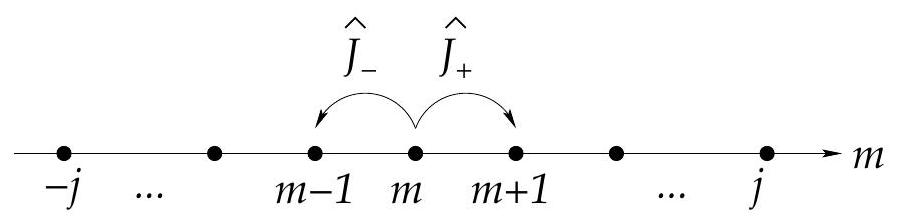
\includegraphics[scale=0.3, center]{2025_05_20_8618f55a41bfe980b4b2g-43}

For ( $S U(3), \cdot$ ) this is quite analogous, but here the states of a multiplet differ by two quantum numbers, $T_{3}$ and $T_{8}$, and not only by one, $m$. One can therefore raise or lower quantum numbers not only in one direction, but in two, as it is schematically (but, as we shall see, not quite correctly) depicted in Fig. 4.1:\\
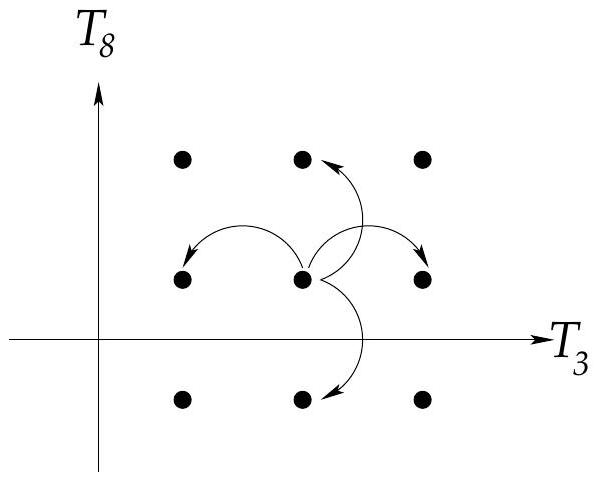
\includegraphics[scale=0.3, center]{2025_05_20_8618f55a41bfe980b4b2g-44}

Figure 4.1: Schematic action of ladder operators on ( $S U(3), \cdot$ ) multiplets.\\
In order to see how this works precisely, let us first define suitable ladder operators:

$$
\begin{aligned}
\hat{T}_{ \pm} & \equiv \hat{T}_{1} \pm i \hat{T}_{2} \\
\hat{V}_{ \pm} & \equiv \hat{T}_{4} \pm i \hat{T}_{5} \\
\hat{U}_{ \pm} & \equiv \hat{T}_{6} \pm i \hat{T}_{7}
\end{aligned}
$$

In addition, we define the so-called hypercharge operator

$$
\hat{Y} \equiv \frac{2}{\sqrt{3}} \hat{T}_{8}=\frac{\hbar}{3}\left(\begin{array}{ccc}
1 & 0 & 0 \\
0 & 1 & 0 \\
0 & 0 & -2
\end{array}\right)
$$

The commutation relations for the ladder operators read:

$$
\begin{aligned}
{\left[\hat{T}_{3}, \hat{T}_{ \pm}\right] } & = \pm \hbar \hat{T}_{ \pm} \\
{\left[\hat{T}_{+}, \hat{T}_{-}\right] } & =2 \hbar \hat{T}_{3}
\end{aligned}
$$

These relations are the same as in the angular momentum algebra for $\hat{L}^{z}$ and the ladder operators $\hat{L}_{ \pm}$. This, in turn, has the consequence that the operators $\left\{\hat{T}_{ \pm}, \hat{T}_{3}\right\}$ define an $(S U(2), \cdot)$ subalgebra (which we had already mentioned above). Furthermore we have:

$$
\begin{aligned}
{\left[\hat{T}_{3}, \hat{V}_{ \pm}\right] } & = \pm \frac{\hbar}{2} \hat{V}_{ \pm} \\
{\left[\hat{T}_{3}, \hat{U}_{ \pm}\right] } & =\mp \frac{\hbar}{2} \hat{U}_{ \pm} \\
{\left[\hat{V}_{+}, \hat{V}_{-}\right] } & =2 \hbar\left(\frac{1}{2} \hat{T}_{3}+\frac{3}{4} \hat{Y}\right) \equiv 2 \hbar \hat{V}_{3} \\
{\left[\hat{U}_{+}, \hat{U}_{-}\right] } & =2 \hbar\left(-\frac{1}{2} \hat{T}_{3}+\frac{3}{4} \hat{Y}\right) \equiv 2 \hbar \hat{U}_{3}
\end{aligned}
$$

where the right-hand sides of the last two equations represent the definitions of the operators $\hat{V}_{3}$ and $\hat{U}_{3}$. We furthermore compute:

$$
\begin{aligned}
{\left[\hat{Y}, \hat{T}_{ \pm}\right] } & =0 \\
{\left[\hat{Y}, \hat{V}_{ \pm}\right] } & = \pm \hbar \hat{V}_{ \pm} \\
{\left[\hat{Y}, \hat{U}_{ \pm}\right] } & = \pm \hbar \hat{U}_{ \pm} \\
{\left[\hat{T}_{ \pm}, \hat{V}_{ \pm}\right] } & =0 \\
{\left[\hat{T}_{ \pm}, \hat{U}_{\mp}\right] } & =0 \\
{\left[\hat{U}_{ \pm}, \hat{V}_{ \pm}\right] } & =0 \\
{\left[\hat{T}_{ \pm}, \hat{V}_{\mp}\right] } & =\mp \hbar \hat{U}_{\mp} \\
{\left[\hat{T}_{ \pm}, \hat{U}_{ \pm}\right] } & = \pm \hbar \hat{V}_{ \pm} \\
{\left[\hat{U}_{ \pm}, \hat{V}_{\mp}\right] } & = \pm \hbar \hat{T}_{\mp} \\
{\left[\hat{T}_{3}, \hat{Y}\right] } & =0
\end{aligned}
$$

The proof of Eqs. (4.22) - 4.37) is left as Exercise 5.\\
With the help of the relations (4.24), (4.25), (4.29), and (4.30) we also derive

$$
\begin{aligned}
{\left[\hat{V}_{3}, \hat{V}_{ \pm}\right] } & =\frac{1}{2}\left[\hat{T}_{3}, \hat{V}_{ \pm}\right]+\frac{3}{4}\left[\hat{Y}, \hat{V}_{ \pm}\right]= \pm \frac{\hbar}{4} \hat{V}_{ \pm} \pm \frac{3}{4} \hbar \hat{V}_{ \pm} \equiv \pm \hbar \hat{V}_{ \pm} \\
{\left[\hat{U}_{3}, \hat{U}_{ \pm}\right] } & =-\frac{1}{2}\left[\hat{T}_{3}, \hat{U}_{ \pm}\right]+\frac{3}{4}\left[\hat{Y}, \hat{U}_{ \pm}\right]= \pm \frac{\hbar}{4} \hat{U}_{ \pm} \pm \frac{3}{4} \hbar \hat{U}_{ \pm} \equiv \pm \hbar \hat{U}_{ \pm}
\end{aligned}
$$

Together with Eqs. (4.26) and (4.27) these equations can be interpreted in the way that the operators $\left\{\hat{V}_{ \pm}, \hat{V}_{3}\right\}$ and $\left\{\hat{U}_{ \pm}, \hat{U}_{3}\right\}$ form two additional $(S U(2), \cdot)$ subalgebras. Since $\hat{V}_{3}$ and $\hat{U}_{3}$ both depend on $\hat{T}_{3}$, these are, however, not independent from the ( $\operatorname{SU}(2), \cdot$ ) subalgebra spanned by $\left\{\hat{T}_{ \pm}, \hat{T}_{3}\right\}$. As we have already mentioned, there is only a single $(S U(2), \cdot)$ subalgebra contained in $(S U(3), \cdot)$.

We now need to clarify how the ladder operators $\hat{T}_{ \pm}, \hat{V}_{ \pm}$, and $\hat{U}_{ \pm}$affect the states of a multiplet. To this end we consider the eigenstates (4.19), or by replacing $T_{8}$ by $Y \equiv$ $\sqrt{3} T_{8} / 2$, the eigenstates

$$
\left|C_{1}, C_{2}, T_{3}, Y\right\rangle \equiv\left|T_{3} Y\right\rangle
$$

where we have abbreviated the list of arguments, since $C_{1}, C_{2}$ cannot be changed by the ladder operators for any given multiplet of $(S U(3), \cdot)$. By definition we have

$$
\begin{aligned}
\hat{T}_{3}\left|T_{3} Y\right\rangle & =T_{3}\left|T_{3} Y\right\rangle \\
\hat{Y}\left|T_{3} Y\right\rangle & =Y\left|T_{3} Y\right\rangle
\end{aligned}
$$

We now conclude that\\
(i) because of Eq. (4.24),

$$
\begin{aligned}
{\left[\hat{T}_{3}, \hat{V}_{ \pm}\right]\left|T_{3} Y\right\rangle } & =\hat{T}_{3} \hat{V}_{ \pm}\left|T_{3} Y\right\rangle-\hat{V}_{ \pm} T_{3}\left|T_{3} Y\right\rangle= \pm \frac{\hbar}{2} \hat{V}_{ \pm}\left|T_{3} Y\right\rangle \\
\Longleftrightarrow \quad \hat{T}_{3} \hat{V}_{ \pm}\left|T_{3} Y\right\rangle & =\left(T_{3} \pm \frac{\hbar}{2}\right) \hat{V}_{ \pm}\left|T_{3} Y\right\rangle
\end{aligned}
$$

This equation means that $\hat{V}_{ \pm}$raises/lowers the eigenvalue $T_{3}$ of a state $\left|T_{3} Y\right\rangle$ by $\hbar / 2$.\\
(ii) because of Eq. 4.25)

$$
\begin{aligned}
{\left[\hat{T}_{3}, \hat{U}_{ \pm}\right]\left|T_{3} Y\right\rangle } & =\hat{T}_{3} \hat{U}_{ \pm}\left|T_{3} Y\right\rangle-\hat{U}_{ \pm} T_{3}\left|T_{3} Y\right\rangle=\mp \frac{\hbar}{2} \hat{U}_{ \pm}\left|T_{3} Y\right\rangle \\
\Longleftrightarrow \quad \hat{T}_{3} \hat{U}_{ \pm}\left|T_{3} Y\right\rangle & =\left(T_{3} \mp \frac{\hbar}{2}\right) \hat{U}_{ \pm}\left|T_{3} Y\right\rangle .
\end{aligned}
$$

This equation means that $\hat{U}_{ \pm}$lowers/raises the eigenvalue $T_{3}$ of a state $\left|T_{3} Y\right\rangle$ by $\hbar / 2$.\\
(iii) because of Eq. 4.29)

$$
\begin{aligned}
{\left[\hat{Y}, \hat{V}_{ \pm}\right]\left|T_{3} Y\right\rangle } & =\hat{Y} \hat{V}_{ \pm}\left|T_{3} Y\right\rangle-\hat{V}_{ \pm} Y\left|T_{3} Y\right\rangle= \pm \hbar \hat{V}_{ \pm}\left|T_{3} Y\right\rangle \\
\Longleftrightarrow \hat{Y} \hat{V}_{ \pm}\left|T_{3} Y\right\rangle & =(Y \pm \hbar) \hat{V}_{ \pm}\left|T_{3} Y\right\rangle
\end{aligned}
$$

This means that $\hat{\boldsymbol{V}}_{ \pm}$raises/lowers the eigenvalue $\boldsymbol{Y}$ of a state $\left|\boldsymbol{T}_{\mathbf{3}} \boldsymbol{Y}\right\rangle$ by $\hbar$.\\
(iv) because of Eq. 4.30

$$
\begin{aligned}
{\left[\hat{Y}, \hat{U}_{ \pm}\right]\left|T_{3} Y\right\rangle } & =\hat{Y} \hat{U}_{ \pm}\left|T_{3} Y\right\rangle-\hat{U}_{ \pm} Y\left|T_{3} Y\right\rangle= \pm \hbar \hat{U}_{ \pm}\left|T_{3} Y\right\rangle \\
\Longleftrightarrow \hat{Y} \hat{U}_{ \pm}\left|T_{3} Y\right\rangle & =(Y \pm \hbar) \hat{U}_{ \pm}\left|T_{3} Y\right\rangle .
\end{aligned}
$$

This means that $\hat{U}_{ \pm}$raises/lowers the eigenvalue $\boldsymbol{Y}$ of a state $\left|T_{3} Y\right\rangle$ by $\hbar$.\\
(v) $\hat{\boldsymbol{T}}_{ \pm}$raises/lowers the eigenvalue $\boldsymbol{T}_{\mathbf{3}}$ of a state $\left|\boldsymbol{T}_{\mathbf{3}} \boldsymbol{Y}\right\rangle$ by $\hbar$.\\
(vi) because of Eq. (4.28) $\hat{\boldsymbol{T}}_{ \pm}$does not change the eigenvalue $\boldsymbol{Y}$ of a state $\left|\boldsymbol{T}_{\mathbf{3}} \boldsymbol{Y}\right\rangle$.

To summarize,\\
(i) $\hat{\boldsymbol{T}}_{ \pm}$raises/lowers $\boldsymbol{T}_{\mathbf{3}}$ by $\hbar$ and leaves $\boldsymbol{Y}$ unchanged.\\
(ii) $\hat{V}_{ \pm}$raises/lowers $T_{3}$ by $\hbar / 2$ and $Y$ by $\hbar$.\\
(iii) $\hat{U}_{ \pm}$lowers/raises $T_{3}$ by $\hbar / 2$ and raises/lowers $Y$ by $\hbar$.

This can be graphically depicted as shown in Fig. 4.2. The red line is the so-called $\boldsymbol{T}$-line. It defines the direction along which the ladder operators $\hat{T}_{ \pm}$act. These change the value of $T_{3}$ by $\pm \hbar$ and leave the value of $Y$ unchanged. The blue line is the so-called $\boldsymbol{V}$-line. It defines the direction along which the ladder operators $\hat{V}_{ \pm}$act. They change $T_{3}$ by $\pm \hbar / 2$ and simultaneously $Y$ by $\pm \hbar$. Finally, the green line is the so-called $\boldsymbol{U}$-line. It defines the direction along which the ladder operators $\hat{U}_{ \pm}$act. These change the value of $T_{3}$ by $\mp \hbar / 2$ and simultaneously $Y$ by $\pm \hbar$.

The way the ladder operators act has the consequence that the states of an ( $\operatorname{SU}(3), \cdot$ ) multiplets do not form a regular lattice in the ( $T_{3}-Y$ ) plane, as shown in Fig. 4.1, but one where states on a line of fixed $Y$ are shifted in $T_{3}$ direction by $\hbar / 2$ with respect to states on a line with $Y \pm \hbar$, as shown in Fig. 4.2,

This information suffices to determine the shape of ( $\boldsymbol{S} \boldsymbol{U}(\mathbf{3}), \cdot$ ) multiplets in the $\left(T_{3}-Y\right)$ plane. To this end let us first remember that\\
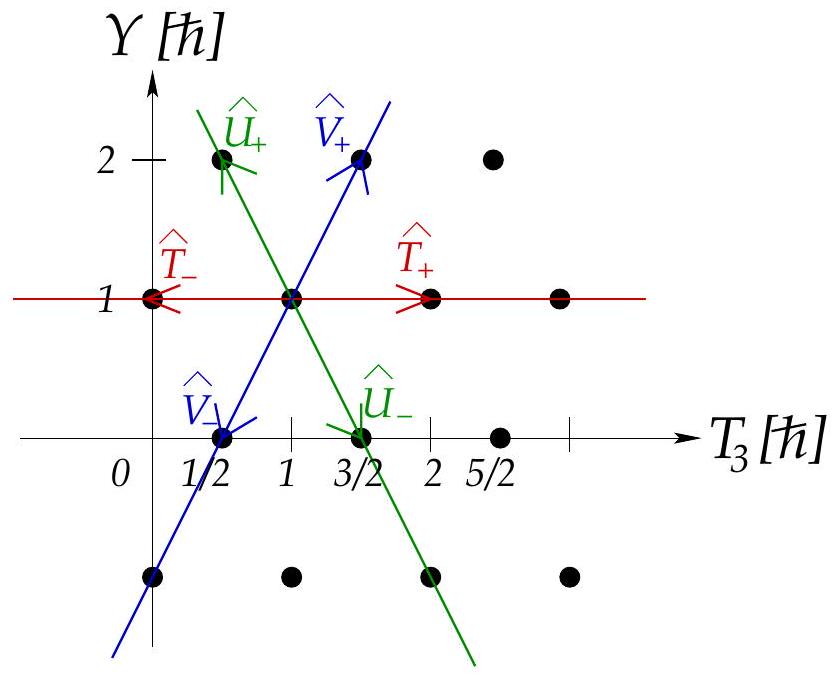
\includegraphics[scale=0.3, center]{2025_05_20_8618f55a41bfe980b4b2g-47}

Figure 4.2: Action of the ladder operators $\hat{T}_{ \pm}, \hat{V}_{ \pm}$, and $\hat{U}_{ \pm}$on states of an $(S U(3), \cdot)$ multiplet.\\
(i) $\left\{\hat{T}_{+}, \hat{T}_{-}, \hat{T}_{3}\right\}$ forms an ( $S U(2), \cdot$ ) subalgebra of ( $S U(3), \cdot$ ), which transforms states of $(S U(2), \cdot)$ multiplets (as parts of $(S U(3), \cdot)$ multiplets) among themselves. Graphically, these ( $S U(2), \cdot$ ) multiplets are located along the (red) $T$-lines in Fig. 4.2 and the ladder operators $\hat{T}_{ \pm}$lead from one state on a $T$-line to the next. While the value of $Y$ always remains the same for these $(S U(2), \cdot)$ multiplets, the value of $T_{3}$ runs between $-T_{3}^{\max }$ and $+T_{3}^{\max }$. This, in turn, implies that these ( $\operatorname{SU}(2), \cdot$ ) multiplets must be located mirror-symmetrically with respect to the $Y$ axis (i.e., the line $T_{3}=0$ ).\\
(ii) $\left\{\hat{V}_{+}, \hat{V}_{-}, \hat{V}_{3}\right\}$ also constitutes an $(S U(2), \cdot)$ subalgebra of $(S U(3), \cdot)$, which transforms the states of ( $S U(2), \cdot$ ) multiplets (as parts of ( $S U(3), \cdot$ ) multiplets) among themselves. However, these ( $S U(2), \cdot$ ) multiplets now lie along the (blue) $V$-lines in Fig. 4.2. When jumping between states with the ladder operators $\hat{V}_{ \pm}$, the value of $V_{3}$ varies between $-V_{3}^{\max }$ and $+V_{3}^{\max }$. This, in turn, implies that these ( $S U(2), \cdot$ ) multiplets must have as many states left as right of the line $V_{3}=0$ or, if we use the definition 4.26) of $\hat{V}_{3}$, of the straight line $Y=-\frac{2}{3} T_{3}$.\\
(iii) $\left\{\hat{U}_{+}, \hat{U}_{-}, \hat{U}_{3}\right\}$ also constitutes an $(S U(2), \cdot)$ subalgebra of $(S U(3), \cdot)$, which transforms the states of ( $S U(2), \cdot$ ) multiplets (as parts of ( $S U(3), \cdot$ ) multiplets) among themselves. However, these ( $S U(2), \cdot$ ) multiplets now lie along the (green) $U$-lines in Fig. 4.2. When jumping between states with the ladder operators $\hat{U}_{ \pm}$, the value of $U_{3}$ varies betweend $-U_{3}^{\max }$ and $+U_{3}^{\max }$. This, in turn, implies that these ( $S U(2), \cdot$ ) multiplets must have as many states left as right of the line $U_{3}=0$ or, if we use the definition 4.27) of $\hat{U}_{3}$, of the straight line $Y=\frac{2}{3} T_{3}$.

The symmetry axes thus identified are shown in Fig. 4.3. The three-fold symmetry only allows three possible geometrical shapes for $(S U(3), \cdot)$ multiplets in the $\left(T_{3}-Y\right)$ plane:\\
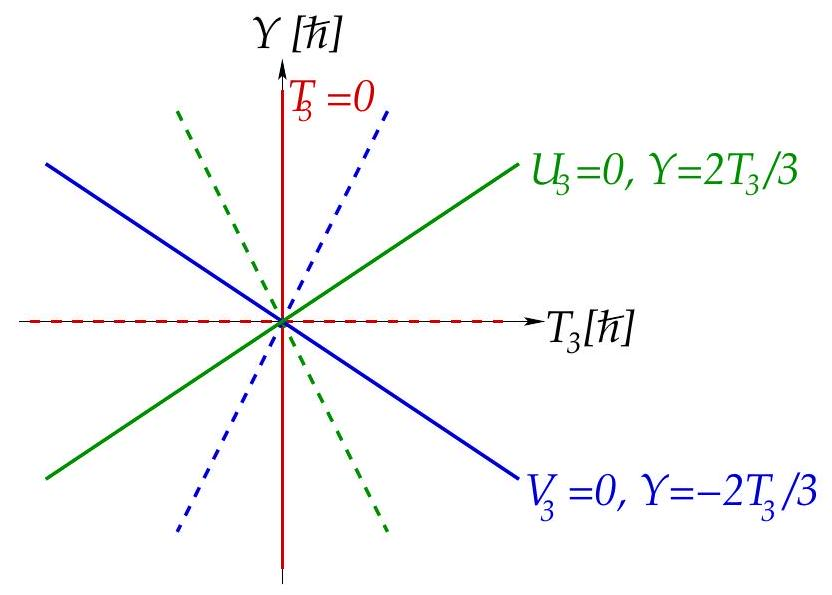
\includegraphics[scale=0.3, center]{2025_05_20_8618f55a41bfe980b4b2g-48}

Figure 4.3: Symmetry axes of ( $S U(3), \cdot$ ) multiplets in the ( $T_{3}-Y$ ) plane (full lines), as well as $T-, V-$, and $U-$ lines (dashed lines).\\
(a) a single state, the so-called singlet located at the origin of the $\left(T_{3}-Y\right)$ plane, i.e., for $T_{3}=Y=0$,\\
(b) triangles centered at the origin of the $\left(T_{3}-Y\right)$ plane,\\
(c) hexagons centered at the origin of the $\left(T_{3}-Y\right)$ plane.

The simplest multiplets which fulfill criteria (a) and (b) are shown in Figs. 4.4 (a-g).

\section{Remarks:}
(i) The number of states of a given multiplet is determined by the following operation: beginning from the upper right (or lower left) corner move with the ladder operators $\hat{T}_{-}\left(\hat{T}_{+}\right)$or $\hat{V}_{-}\left(\hat{V}_{+}\right)$, respectively, to the adjacent state. From there use $\hat{T}_{-}\left(\hat{T}_{+}\right)$, $\hat{V}_{-}\left(\hat{V}_{+}\right)$, or $\hat{U}_{+}\left(\hat{U}_{-}\right)$to move to the next possible state inside a given triangle. One cannot leave the triangle, but in this way one can also reach states inside the triangle. Finally, this prescription defines a lattice of states on the sides and inside the triangle. Counting the states, one obtains the total number of states in a given multiplet.\\
(ii) Counting along $T$-lines, the triplet [3] contains a $T$-singlet and a $T$-doublet or, counting along $V$-lines, a $V$-singlet and a $V$-doublet or, counting along $U$-lines, a $U$-singlet and a $U$-doublet, respectively. An analogous argument holds for the multiplet which is conjugate to the triplet, the so-called anti-triplet $[\overline{3}]$.\\[0pt]
(iii) The sextet [6] contains a $T$-singlet, a $T$-doublet, and a $T$-triplet, or a $V$-singlet, a $V$-doublet, and a $V$-triplet, or a $U$-singlet, a $U$-doublet, and a $U$-triplet, respectively. An analogous argument holds for the anti-sextet $[\overline{\mathbf{6}}]$.\\
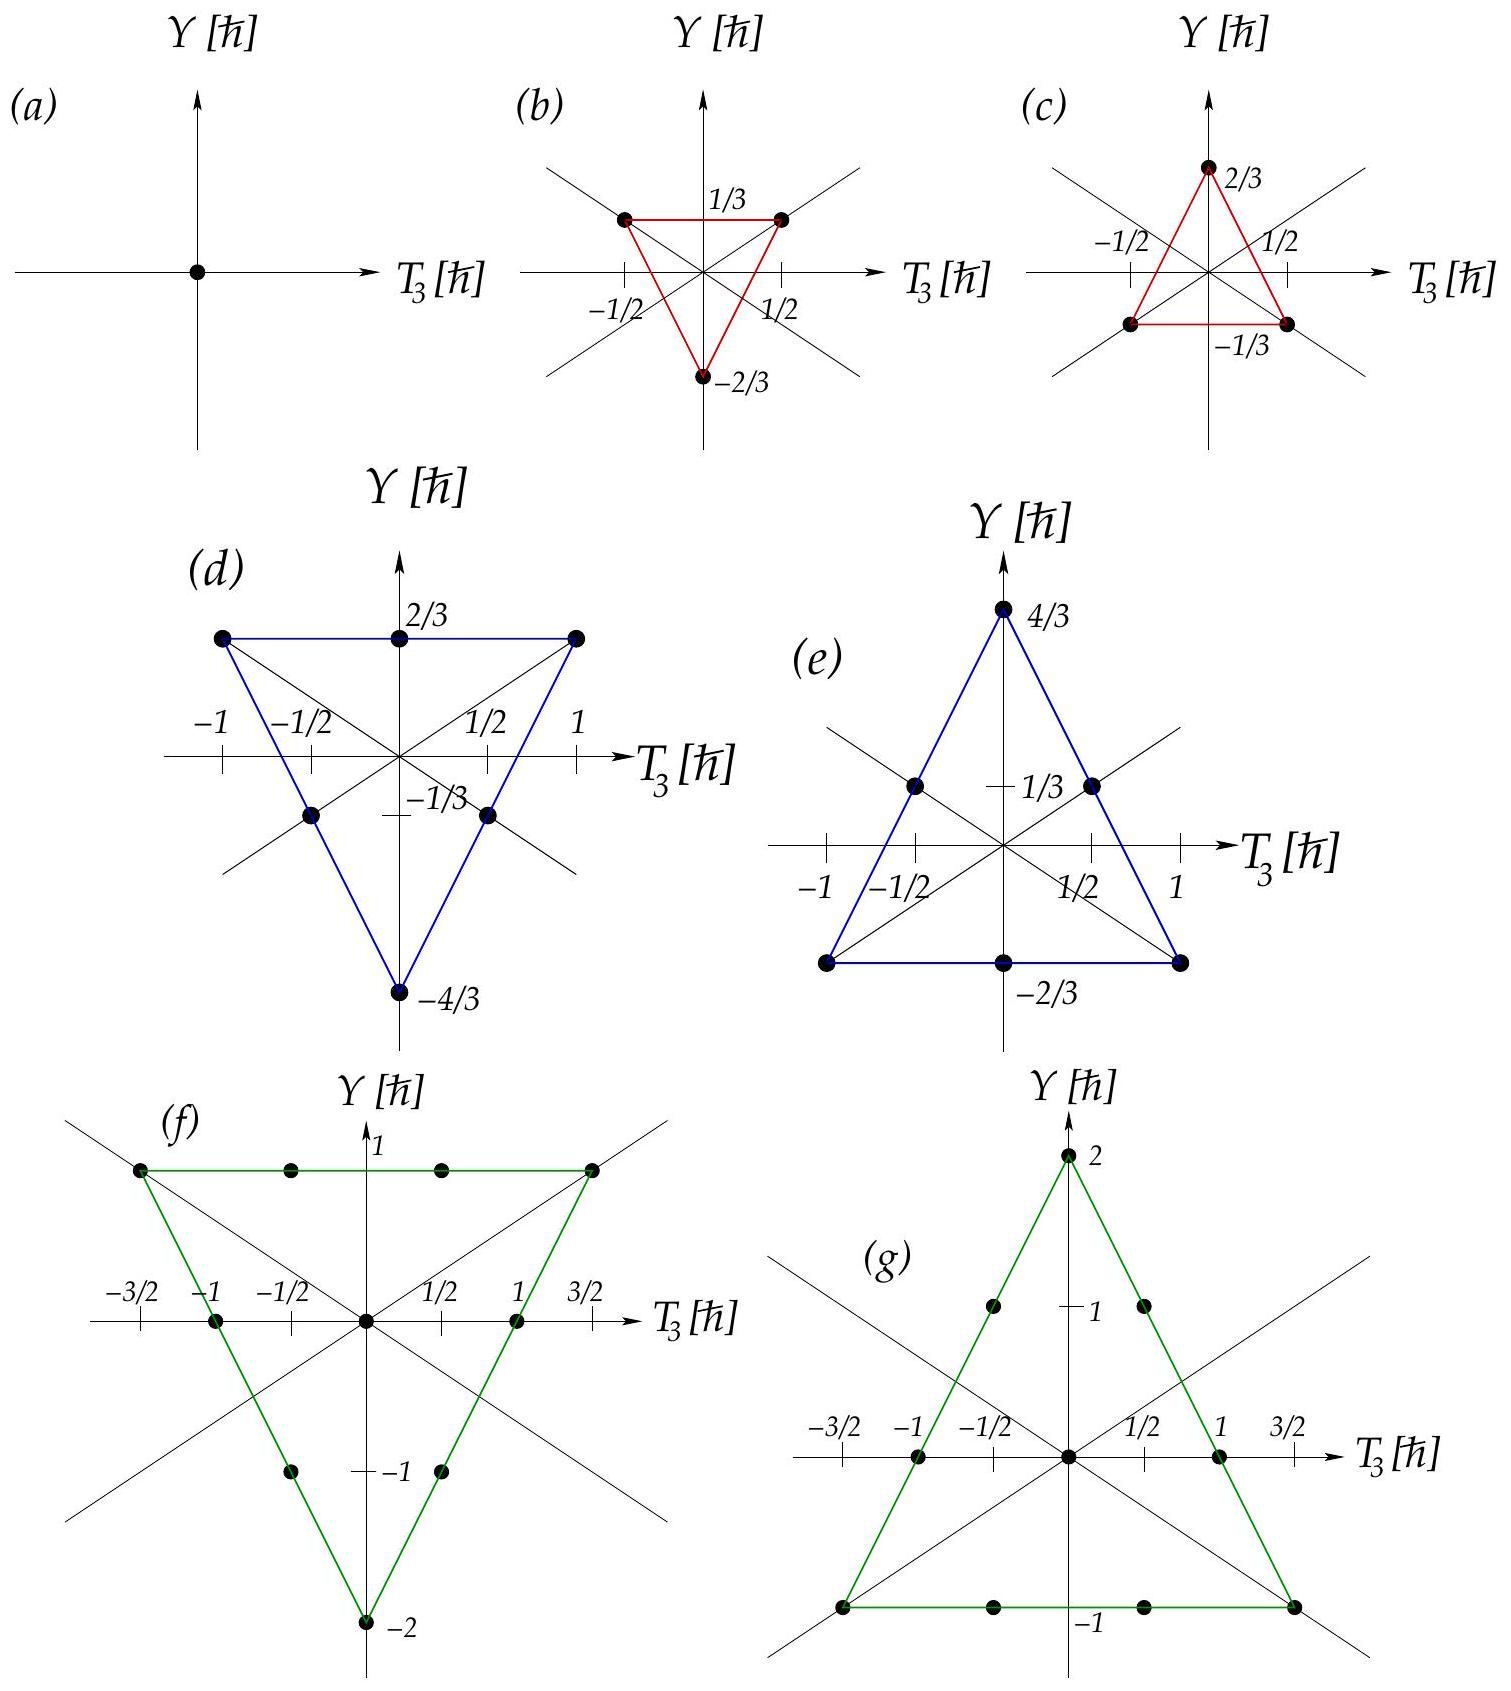
\includegraphics[scale=0.3, center]{2025_05_20_8618f55a41bfe980b4b2g-49}

Figure 4.4: (a) Singlet [1], (b) triplet [3], (c) anti-triplet [3], (d) sextet [6], (e) anti-sextet $[\overline{6}]$, (f) decuplet [10], and (g) anti-decuplet [10].\\[0pt]
(iv) The decuplet [10] contains a $T$-singlet, a $T$-doublet, a $T$-triplet, and a $T$-quadruplet, or a $V$-singlet, a $V$-doublet, a $V$-triplet, and a $V$-quadruplet, or a $U$-singlet, a $U$-doublet, a $U$-triplet, and a $U$-quadruplet, respectively. An analogous argument holds for the anti-decuplet $[\overline{\mathbf{1 0}}]$.\\[0pt]
(v) The triplet [3] with three possible states corresponds to the fundamental representation of $(S U(3), \cdot)$. We will see in the next section that we can generate the\\
singlet, the anti-triplet, as well as all higher-dimensional multiplets by coupling a suitable number of triplets together.

The simplest multiplet obeying criterium (c) is the octet [8] shown in Fig. 4.5, This is the adjoint representation of $(S U(3), \cdot)$.\\
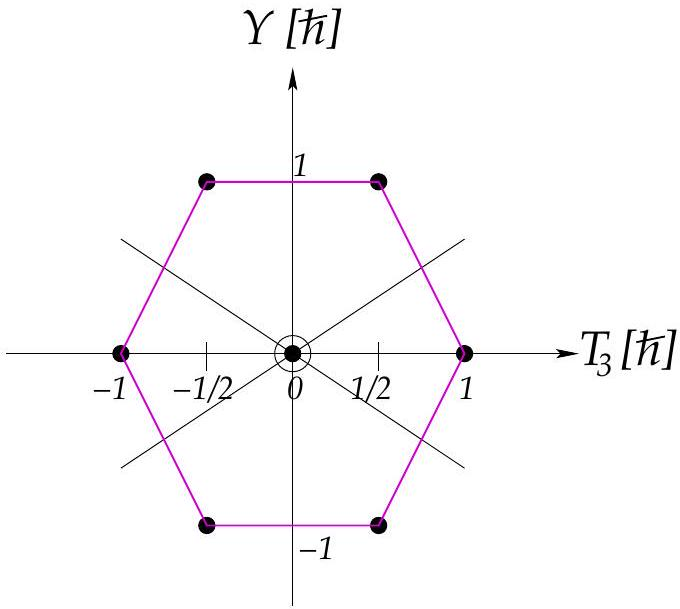
\includegraphics[scale=0.3, center]{2025_05_20_8618f55a41bfe980b4b2g-50}

Figure 4.5: Octet [8].

\section{Remarks:}
(i) The anti-octet $[\overline{\boldsymbol{8}}]$ has the same shape as the octet. One says that $[\overline{8}]$ and [8] self-conjugate.\\
(ii) From Fig. 4.5 one observes that the octet contains two $T$-doublets and a $T$-triplet, or two $V$-doublets and a $V$-triplet, or two $U$-doublets and a $U$-triplet, respectively.\\
(iii) This yields only seven states. So why does one speak of an "octet", i.e., a multiplet with eight states? The reason is that the origin is doubly occupied with two different states, namely with one state of the triplet and an additional singlet. This is indicated by an additional circle around the origin in Fig. 4.5.

What is the reason for this double occupancy? Starting from the state $\mid T_{3}=1 Y=$ $0\rangle$, one can reach the origin in three different ways:

$$
\begin{aligned}
|00\rangle_{\mathrm{I}} & \sim \hat{T}_{-}|10\rangle, \\
|00\rangle_{\mathrm{II}} & \sim \hat{V}_{-} \hat{U}_{+}|10\rangle \sim \hat{V}_{-}\left|\frac{1}{2} 1\right\rangle, \\
|00\rangle_{\mathrm{III}} & \sim \hat{U}_{+} \hat{V}_{-}|10\rangle \sim \hat{U}_{+}\left|\frac{1}{2}-1\right\rangle .
\end{aligned}
$$

These different ways are shown graphically in Fig. 4.6,\\
However, because of Eq. (4.36) $\hat{U}_{+} \hat{V}_{-}=\hat{V}_{-} \hat{U}_{+}+\hbar \hat{T}_{-}$, way III is not linearly independent of way I and way II,

$$
|00\rangle_{\mathrm{III}} \sim \hat{U}_{+} \hat{V}_{-}|10\rangle=\hat{V}_{-} \hat{U}_{+}|10\rangle+\hbar \hat{T}_{-}|10\rangle=\alpha|00\rangle_{\mathrm{II}}+\beta|00\rangle_{\mathrm{I}} .
$$

\begin{center}
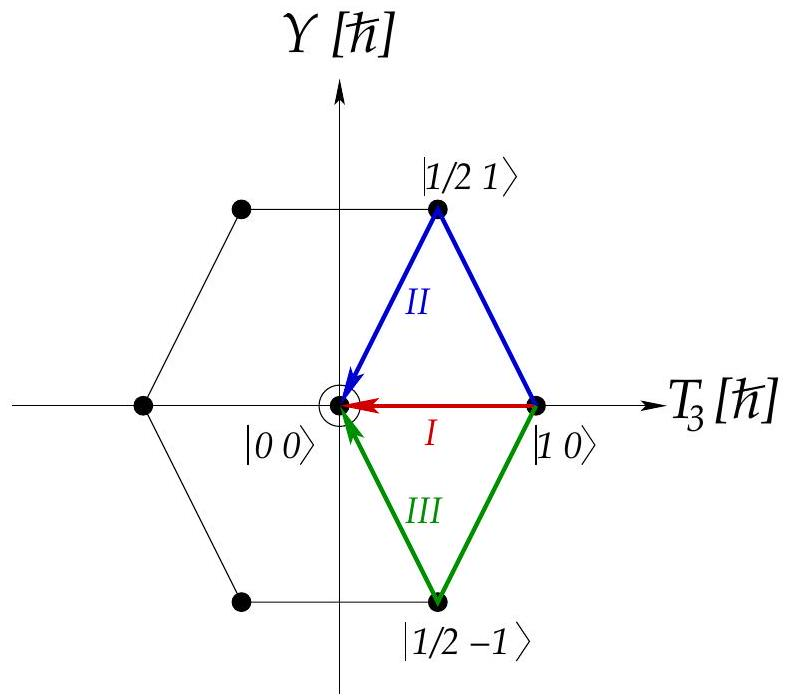
\includegraphics[scale=0.3]{2025_05_20_8618f55a41bfe980b4b2g-51}
\end{center}

Figure 4.6: The three different ways to reach the origin $|00\rangle$ starting from $|10\rangle$.

Thus, the octet has two linearly independent states, $|00\rangle_{\mathrm{I}}$ and $|00\rangle_{\mathrm{II}}$, which are located at the origin.

The rule of multiple occupancy or degeneracy of states with the same quantum numbers $T_{3}$ and $Y$ can be generalized to arbitrary multiplets. In general, the degeneracy of states on each inner shell is by one unit larger than those of the states on the adjacent outer shell. The degeneracy of the outermost shell is always equal to one. An example is shown in Fig. 4.7.

This rule holds as long as a shell is not a triangle. Inside a triangle the degeneracy does not increase any more, but stays constant. The reason is that there is now only one linearly independent way to reach a point inside a triangle. To understand this, let us consider the decuplet, Fig. 4.8.

At first glance, one would think that, starting from state $|10\rangle$, there are three different ways to reach the origin $|00\rangle$, just like for the octet. For the same reasons as for the octet, at least two of them should be linearly independent, e.g.

$$
|00\rangle_{\mathrm{I}} \sim \hat{T}_{-}|10\rangle \quad \text { and } \quad|00\rangle_{\mathrm{II}} \sim \hat{V}_{-} \hat{U}_{+}|10\rangle,
$$

so that the origin is again doubly occupied. However, it holds

$$
|10\rangle \sim \hat{V}_{-}\left|\frac{3}{2} 1\right\rangle
$$

and therefore

$$
\begin{aligned}
|00\rangle_{\mathrm{II}} & \sim \hat{V}_{-} \hat{U}_{+} \hat{V}_{-}\left|\frac{3}{2} 1\right\rangle=\hat{V}_{-}\left(\hat{V}_{-} \hat{U}_{+}+\hbar \hat{T}_{-}\right)\left|\frac{3}{2} 1\right\rangle \\
& =\left(\hat{V}_{-}\right)^{2} \hat{U}_{+}\left|\frac{3}{2} 1\right\rangle+\hbar \hat{V}_{-} \hat{T}_{-}\left|\frac{3}{2} 1\right\rangle \equiv \hbar \hat{V}_{-} \hat{T}_{-}\left|\frac{3}{2} 1\right\rangle \\
& =\hbar \hat{T}_{-} \hat{V}_{-}\left|\frac{3}{2} 1\right\rangle=\hat{T}_{-}\left(\hbar \hat{V}_{-}\left|\frac{3}{2} 1\right\rangle\right) \\
& \sim \hat{T}_{-}|10\rangle \sim|00\rangle_{\mathrm{I}} .
\end{aligned}
$$

\begin{center}
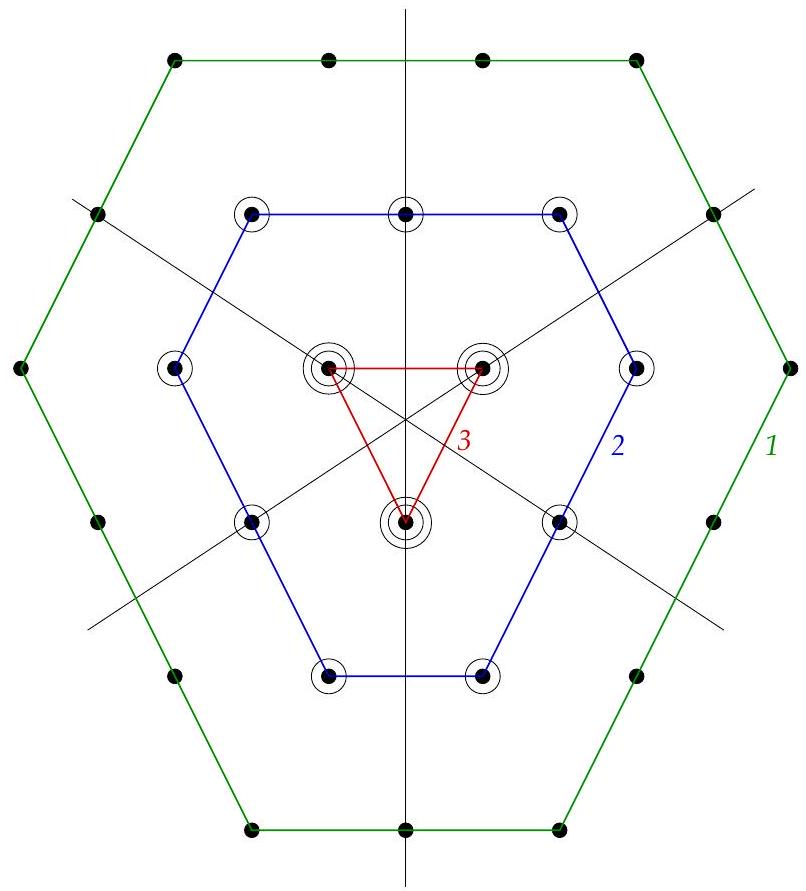
\includegraphics[scale=0.3]{2025_05_20_8618f55a41bfe980b4b2g-52(1)}
\end{center}

Figure 4.7: Starting from the outermost shell, the degeneracy of states increases by one as one moves from one inner shell to the next.\\
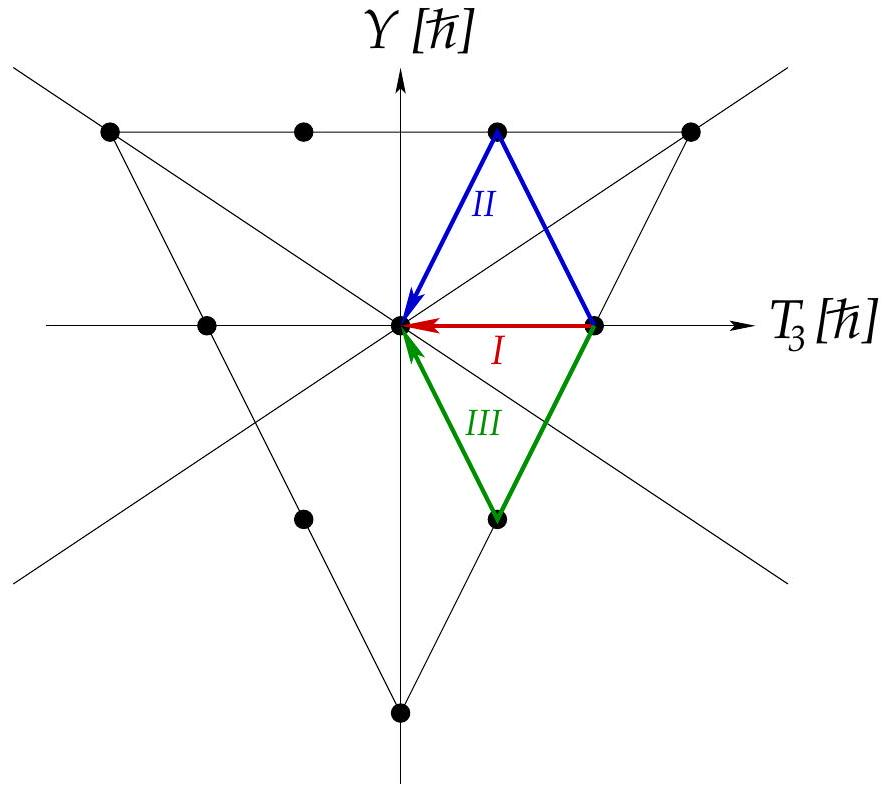
\includegraphics[scale=0.3, center]{2025_05_20_8618f55a41bfe980b4b2g-52}

Figure 4.8: The three ways to reach the origin $|00\rangle$, starting from state $|10\rangle$.

Here we have made use of Eqs. (4.31) and (4.36), and employed the fact that the state $\left|\frac{3}{2} 1\right\rangle$ is the state with the maximum hypercharge $Y=1$ in the multiplet, such that $\hat{U}_{+}\left|\frac{3}{2} 1\right\rangle \equiv 0$, since this operation would lead outside the multiplet, which is not allowed.

Equation (4.44) thus shows that $|00\rangle_{\mathrm{II}} \sim|00\rangle_{\mathrm{I}}$, i.e., these two states are not linearly independent from each other, thus not different. Another way to see this is, starting from $\left|\frac{3}{2} 1\right\rangle$, to apply either $\hat{T}_{-} \hat{V}_{-}$or $\hat{V}_{-} \hat{T}_{-}$in order to reach $|00\rangle$. Because of Eq. 4.31) this is, however, the same, thus not linearly independent.

\subsection{Construction of multiplets from the fundamental representation}
In the theory of coupling of angular momenta, two angular momenta (or spins, respectively) are coupled or "added" to form states with a certain total angular momentum. From the mathematical point of view, one takes the product space of the two angular momenta and decomposes it in terms of multiplets for given total angular momentum (or spin, respectively). This process is called reduction.

It stands to reason that, by coupling together sufficiently many smallest non-trivial angular momenta (or spins, respectively), it should be possible to generate all higherdimensional multiplets. This is indeed the case: by coupling together sufficiently many fundamental representations of ( $S U(2), \cdot$ ), i.e., doublets, all higher multiplets for given angular momentum (or spin, respectively) can be generated. We show this at hand of two examples:

$$
\text { (i) } \begin{aligned}
& j_{1}=\frac{1}{2} \text { with } j_{2}=\frac{1}{2} \Longrightarrow j=0 \text { and } j=1 \\
& \uparrow \quad \otimes \quad \uparrow \quad \Longrightarrow \quad \uparrow \downarrow \text { and } \quad \uparrow
\end{aligned}
$$

This relation can be simply written with the notation "doublet $=[2]$ ", "singlet $=[1]$ ", and "triplet $=[3]$ " as

$$
[2] \otimes[2]=[1] \oplus[3]
$$

This process can be continued, by coupling the doublet to a triplet:\\
(ii) $\quad j_{1}=\frac{1}{2} \quad$ with $\quad j_{2}=1 \quad \Longrightarrow \quad j=\frac{1}{2} \quad$ and $\quad j=\frac{3}{2}$\\
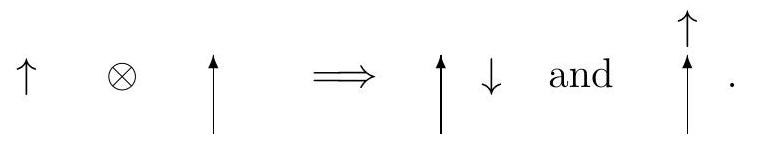
\includegraphics[scale=0.3, center]{2025_05_20_8618f55a41bfe980b4b2g-53}

With the notation "quadruplet $=[4]$ " this can be succinctly written as

$$
[2] \otimes[3]=[2] \oplus[4]
$$

By coupling a doublet or triplet to the quadruplet, one can continue this process and in this way generate all higher-dimensional multiplets.

There is a graphical method to perform this reduction. To this end, we draw the first doublet onto the $J_{3}$ axis:

4 The group ( $\boldsymbol{S U} \mathbf{( 3 ) , ~} \cdot$ )\\
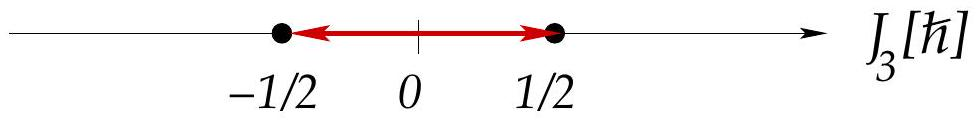
\includegraphics[scale=0.3, center]{2025_05_20_8618f55a41bfe980b4b2g-54(3)}

Now we put the second doublet with its center ( $J_{3}=0$ ) onto each of the two states $J_{3}=1 / 2$ and $J_{3}=-1 / 2$ (in units of $\hbar$ ) of the first doublet:\\
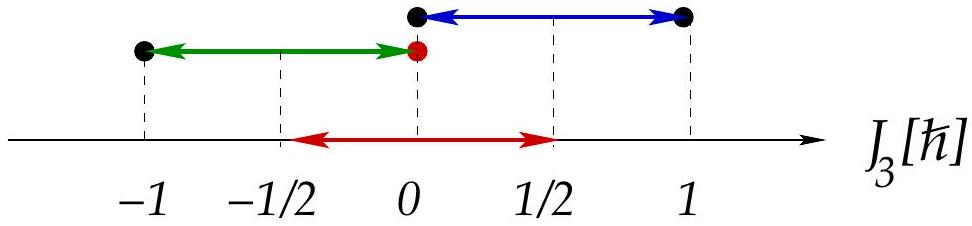
\includegraphics[scale=0.3, center]{2025_05_20_8618f55a41bfe980b4b2g-54(1)}

This generates once the states $J_{3}=1$ and $J_{3}=-1$, as well as twice the state $J_{3}=0$. This just corresponds to one singlet, $J=0$ or [1] (red dot), and one triplet, $J=1$ or [3] (black dots).

If one repeats this with another doublet and the triplet, one obtains a doublet, $J=1 / 2$ or [2] (red dots), and a quadruplet, $J=3 / 2$ or [4] (black dots):\\
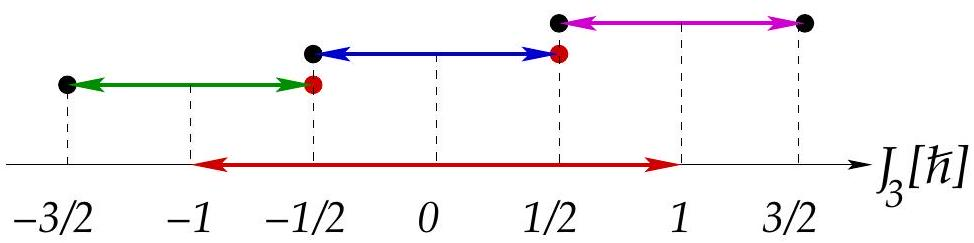
\includegraphics[scale=0.3, center]{2025_05_20_8618f55a41bfe980b4b2g-54(2)}

Analogously, one can generate all ( $S U(3), \cdot$ ) multiplets by coupling, starting from the fundamental representation, the triplet. As a first example, we consider the coupling of two triplets:\\
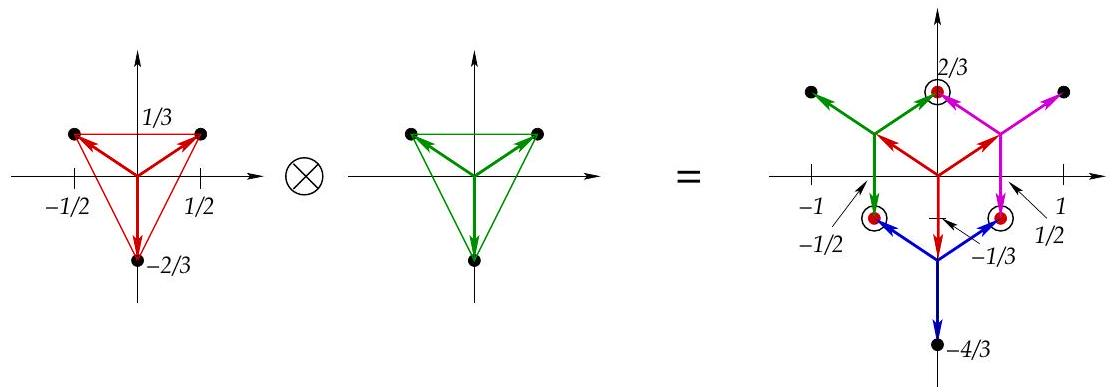
\includegraphics[scale=0.3, center]{2025_05_20_8618f55a41bfe980b4b2g-54(4)}\\
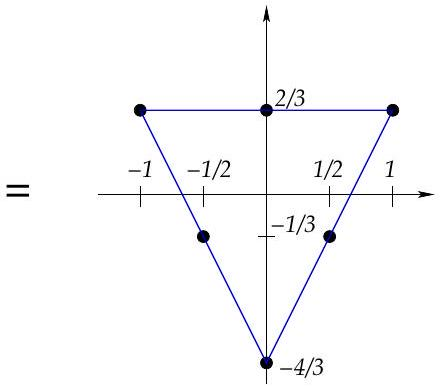
\includegraphics[scale=0.3, center]{2025_05_20_8618f55a41bfe980b4b2g-54(5)}\\
$\oplus$\\
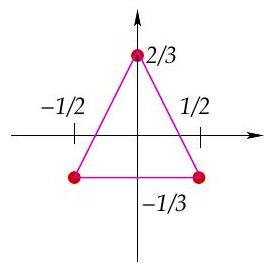
\includegraphics[scale=0.3, center]{2025_05_20_8618f55a41bfe980b4b2g-54}

This yields a sextet and an anti-triplet,

$$
[3] \otimes[3]=[\overline{3}] \oplus[6] .
$$

Now we couple the anti-triplet to another triplet:\\
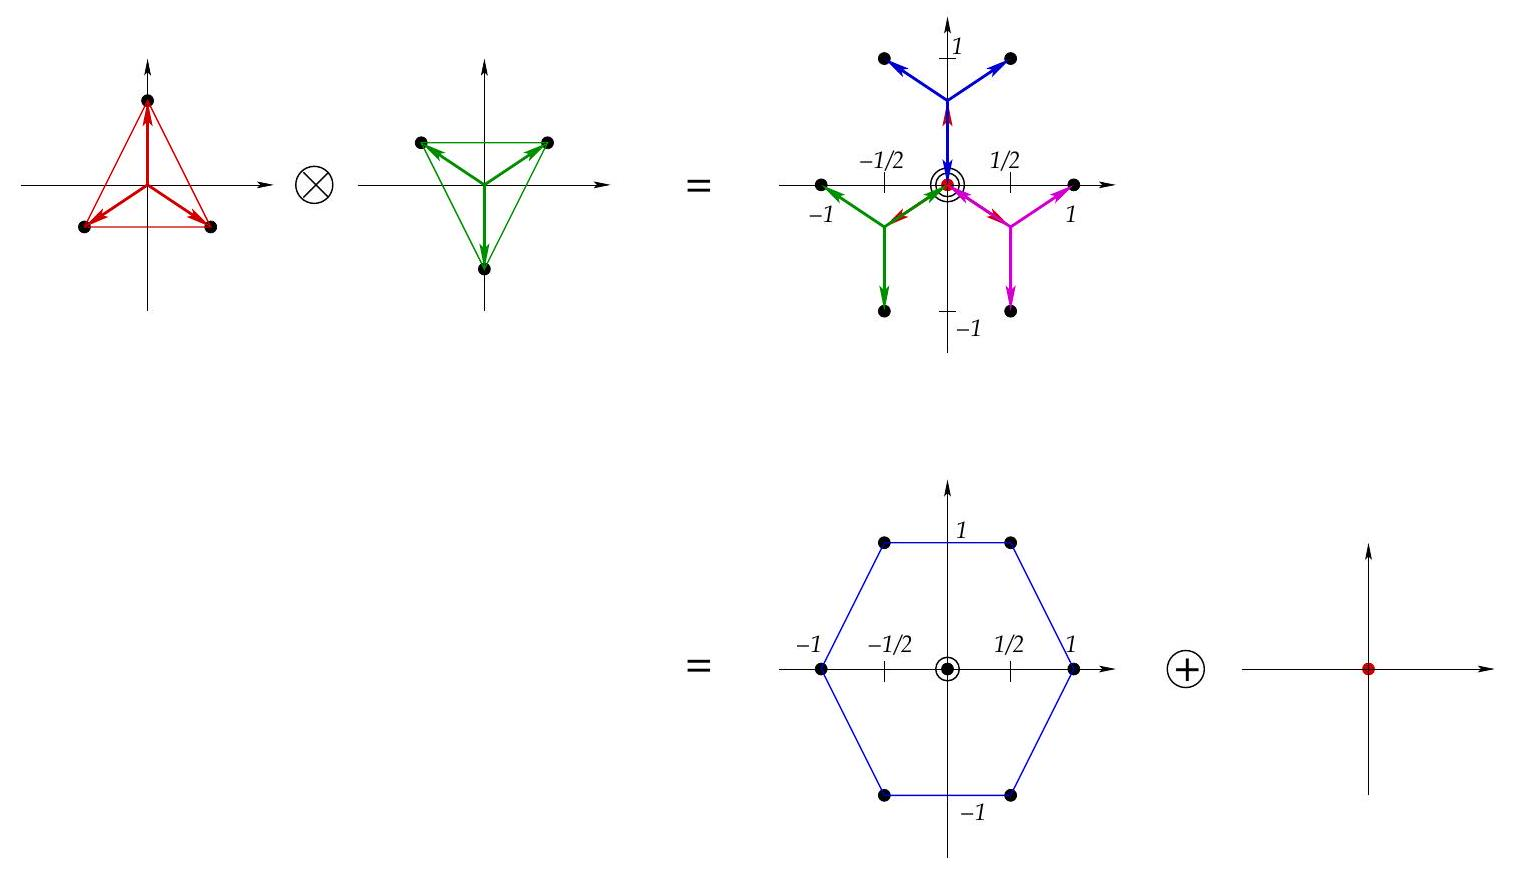
\includegraphics[scale=0.3, center]{2025_05_20_8618f55a41bfe980b4b2g-55(2)}

This yields an octet and a singlet,

$$
[\overline{3}] \otimes[3]=[1] \oplus[8]
$$

Starting from the sextet, we obtain by coupling it to another triplet:\\
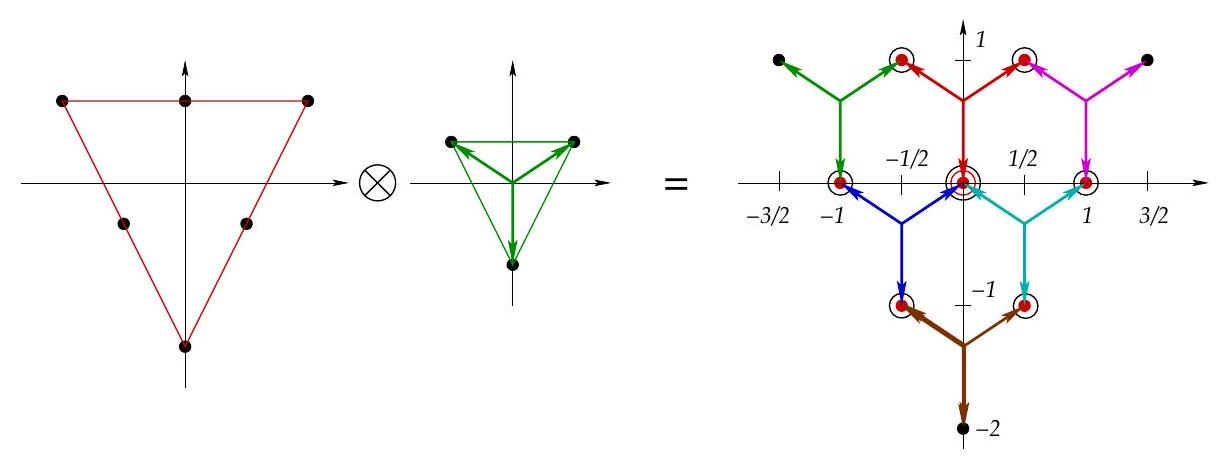
\includegraphics[scale=0.3, center]{2025_05_20_8618f55a41bfe980b4b2g-55(1)}\\
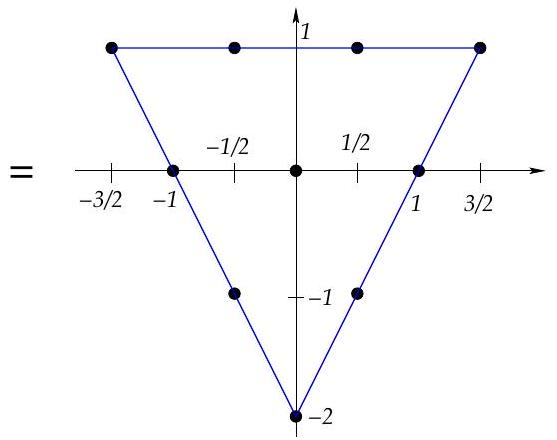
\includegraphics[scale=0.3, center]{2025_05_20_8618f55a41bfe980b4b2g-55(3)}\\
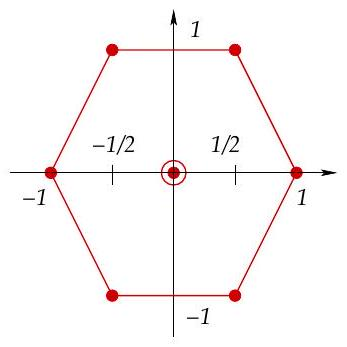
\includegraphics[scale=0.3, center]{2025_05_20_8618f55a41bfe980b4b2g-55}

4 The group ( $\boldsymbol{S U} \mathbf{( 3 ) ,} \cdot$ )

This yields a decuplet and an octet,

$$
[3] \otimes[6]=[8] \oplus[10] .
$$

We can use rules (4.49), 4.50, and 4.51) together with the law of associativity to determine more complex couplings, e.g.\\
$[3] \otimes[3] \otimes[3]=[3] \otimes([\overline{3}] \oplus[6])=([3] \otimes[\overline{3}]) \oplus([3] \otimes[6])=[1] \oplus[8] \oplus[8] \oplus[10]$.

\subsection{Young Tableaux}

\section{Unitary symmetries of the strong interaction}

\section{U(1) symmetry of quantum electrodynamics}
Symmetries play a prominent role in modern theories of the Forces of Nature. This is especially true for the theory of the strong interaction. Before turning to this theory, however, let us first consider the (simpler) theory of electromagnetism, quantum electrodynamics (QED), which describes the interactions between electrons and photons. The respective Lagrangian reads (in natural units, $\hbar=c=1$ )

$$
\mathcal{L}_{\mathrm{QED}}=-\frac{1}{4} F^{\mu \nu} F_{\mu \nu}+\bar{\psi}(i \not D-m) \psi
$$

where $F^{\mu \nu}=\partial^{\mu} A^{\nu}-\partial^{\nu} A^{\mu}$ is the field-strength tensor of the electromagnetic field, with the 4 -vector potential $A^{\mu}$, the so-called gauge field, and the covariant derivative

$$
D_{\mu}=\partial_{\mu}-i e A_{\mu}
$$

The quantity $\psi$ is the 4 -spinor of the electron and $m$ its mass. The first term in the Lagrangian (5.1) is the so-called gauge-field term, which describes the dynamics of the gauge field $A^{\mu}$, in this case the photon field. The second term is the so-called matter term, which describes the dynamics of the matter fields, in this case the electron.

The Lagrangian (5.1) is invariant under so-called ( $U(1), \cdot$ ) gauge transformations,

$$
\begin{aligned}
\psi & \longrightarrow \psi^{\prime}=\hat{U} \psi \\
A^{\mu} & \longrightarrow A^{\prime \mu}=\hat{U} A^{\mu} \hat{U}^{-1}-\frac{i}{e}\left(\partial^{\mu} \hat{U}\right) \hat{U}^{-1}
\end{aligned}
$$

where

$$
\hat{U} \equiv e^{i e \Lambda(X)} \in U(1)
$$

is a space-time dependent phase factor, and at the same time a representation of an element of the group $(\boldsymbol{U}(1), \cdot)$. For elements of $(U(1), \cdot)$ Eq. (5.4) simplifies as follows:

$$
A^{\mu} \longrightarrow A^{\prime \mu}=A^{\mu}+\partial^{\mu} \Lambda
$$

The invariance of the Lagrangian (5.1) under the transformations (5.3), (5.4) is seen as follows:\\
(i) The field-strength tensor is invariant under the transformation (5.4),

$$
F^{\mu \nu} \longrightarrow F^{\prime \mu \nu}=\partial^{\mu}\left(A^{\nu}+\partial^{\nu} \Lambda\right)-\partial^{\nu}\left(A^{\mu}+\partial^{\mu} \Lambda\right)=F^{\mu \nu}
$$

as long as $\Lambda(X)$ is twice continuously differentiable, $\partial^{\mu} \partial^{\nu} \Lambda=\partial^{\nu} \partial^{\mu} \Lambda$. Consequently, also the gauge-field term in Eq. 5.1 is invariant.\\
(ii) The covariant derivative of the matter field transforms as the matter field itself,

$$
\begin{aligned}
D_{\mu} \psi \longrightarrow D_{\mu}^{\prime} \psi^{\prime} & =\left(\partial_{\mu}-i e A_{\mu}^{\prime}\right) \psi^{\prime}=\left[\partial_{\mu}-i e A_{\mu}-i e\left(\partial_{\mu} \Lambda\right)\right] e^{i e \Lambda} \psi \\
& =e^{i e \Lambda}\left[\partial_{\mu}+i e\left(\partial_{\mu} \Lambda\right)-i e A_{\mu}-i e\left(\partial_{\mu} \Lambda\right)\right] \psi \\
& =e^{i e \Lambda}\left(\partial_{\mu}-i e A_{\mu}\right) \psi \equiv e^{i e \Lambda} D_{\mu} \psi
\end{aligned}
$$

Therefore, also the matter term in Eq. (5.1) is invariant,

$$
\bar{\psi}(i \not D-m) \psi \longrightarrow \bar{\psi}^{\prime}\left(i \not D^{\prime}-m\right) \psi^{\prime}=\bar{\psi} e^{-i e \Lambda} e^{i e \Lambda}(i \not D-m) \psi=\bar{\psi}(i \not D-m) \psi .
$$

Gauge transformations are also termed local symmetry transformations and one speaks of local invariance under these transformations or, short, of a local symmetry. The special case $\Lambda(X)=$ const. corresponds to global symmetry transformations or global invariance or global symmetry, respectively.

\section{SU(3) color symmetry of quantum chromodynamics}
The theory of the strong interaction is quantum chromodynamics (QCD) (greek: $\chi \rho \widetilde{\omega} \mu \alpha=$ color). It describes the interaction between quarks and gluons. The Lagrangian of QCD looks quite similar to that of QED, Eq. 5.1,

$$
\mathcal{L}_{\mathrm{QCD}}=-\frac{1}{2} \operatorname{Tr}\left(\mathcal{F}^{\mu \nu} \mathcal{F}_{\mu \nu}\right)+\bar{\Psi}(i \not D-\hat{m}) \Psi
$$

Here,

$$
\mathcal{F}^{\mu \nu} \equiv F_{a}^{\mu \nu} \hat{T}_{a}
$$

is the matrix-valued field-strength tensor, with the eight generators $\hat{T}_{a}$ of $(S U(3), \cdot)$ in the fundamental representation, i.e., as $(3 \times 3)$ matrices, cf. Eq. (4.2). $\Psi$ is the quark field and $\hat{m}$ its mass.

Using Eq. (3.41) the gauge-field term of QCD can be brought into a similar form as that of QED,

$$
\frac{1}{2} \operatorname{Tr}\left(\mathcal{F}^{\mu \nu} \mathcal{F}_{\mu \nu}\right)=F_{a}^{\mu \nu} F_{\mu \nu}^{b} \frac{1}{2} \operatorname{Tr}\left(\hat{T}_{a} \hat{T}_{b}\right)=\frac{1}{4} F_{a}^{\mu \nu} F_{\mu \nu}^{b} \delta_{a b}=\frac{1}{4} F_{a}^{\mu \nu} F_{\mu \nu}^{a}
$$

The difference to QED is that there are now eight different field-strength tensors $F_{a}^{\mu \nu}$, corresponding to the eight colors of the gluon fields. There is, however, another, less obvious, difference between the field-strength tensors of QCD and that of QED. Up to a factor $i / g$, where $g$ is the coupling constant of the strong interaction, the field-strength tensor can be defined in terms of the commutator,

$$
\mathcal{F}^{\mu \nu} \equiv \frac{i}{g}\left[D^{\mu}, D^{\nu}\right]
$$

of two covariant derivatives

$$
D_{\mu}=\partial_{\mu}-i g \mathcal{A}_{\mu}
$$

where the covariant derivative is matrix-valued, just as the field-strength tensor, with the matrix-valued 4 -vector potential, or gauge field, respectively,

$$
\mathcal{A}^{\mu} \equiv A_{a}^{\mu} \hat{T}_{a}
$$

The eight 4 -vector potentials $A_{a}^{\mu}$ correspond to the eight gluon fields. We compute the commutator (5.8) explicitly,

$$
\begin{aligned}
\frac{i}{g}\left[D^{\mu}, D^{\nu}\right]= & \frac{i}{g}\left[\left(\partial^{\mu}-i g \mathcal{A}^{\mu}\right)\left(\partial^{\nu}-i g \mathcal{A}^{\nu}\right)-\left(\partial^{\nu}-i g \mathcal{A}^{\nu}\right)\left(\partial^{\mu}-i g \mathcal{A}^{\mu}\right)\right] \\
= & \frac{i}{g}\left[\partial^{\mu} \partial^{\nu}-i g\left(\partial^{\mu} \mathcal{A}^{\nu}\right)-i g \mathcal{A}^{\nu} \partial^{\mu}-i g \mathcal{A}^{\mu} \partial^{\nu}-g^{2} \mathcal{A}^{\mu} \mathcal{A}^{\nu}\right. \\
& \left.-\partial^{\nu} \partial^{\mu}+i g\left(\partial^{\nu} \mathcal{A}^{\mu}\right)+i g \mathcal{A}^{\mu} \partial^{\nu}+i g \mathcal{A}^{\nu} \partial^{\mu}+g^{2} \mathcal{A}^{\nu} \mathcal{A}^{\mu}\right] \\
= & \partial^{\mu} \mathcal{A}^{\nu}-\partial^{\nu} \mathcal{A}^{\mu}-i g\left[\mathcal{A}^{\mu}, \mathcal{A}^{\nu}\right] \\
= & \partial^{\mu} \mathcal{A}^{\nu}-\partial^{\nu} \mathcal{A}^{\mu}-i g A_{b}^{\mu} A_{c}^{\nu}\left[\hat{T}^{b}, \hat{T}^{c}\right] \\
= & \left(\partial^{\mu} A_{a}^{\nu}-\partial^{\nu} A_{a}^{\nu}+g f_{a b c} A_{b}^{\mu} A_{c}^{\nu}\right) \hat{T}_{a}
\end{aligned}
$$

where we used the Lie algebra (4.11) of ( $S U(3), \cdot$ ) in the last step. Comparing this result with Eq. (5.7), we realize that

$$
F_{a}^{\mu \nu} \equiv \partial^{\mu} A_{a}^{\nu}-\partial^{\nu} A_{a}^{\mu}+g f_{a b c} A_{b}^{\mu} A_{c}^{\nu}
$$

The non-abelian nature of the group ( $S U(3), \cdot$ ) causes additional terms in the fieldstrength tensor of the $a$ th gluon, which depend on the gluon fields with colors $b$ and $c$. These non-abelian terms lead to 3- and 4-gluon interaction terms in the gauge-field term of the QCD Lagrangian,

$$
\begin{aligned}
-\frac{1}{4} F_{a}^{\mu \nu} F_{\mu \nu}^{a}= & -\frac{1}{2} \partial^{\mu} A_{a}^{\nu}\left(\partial_{\mu} A_{\nu}^{a}-\partial_{\nu} A_{\mu}^{a}\right) \\
& -g f_{a b c} \partial^{\mu} A_{a}^{\nu} A_{\mu}^{b} A_{\nu}^{c}-\frac{g^{2}}{4} f_{a b c} f_{a d e} A_{b}^{\mu} A_{c}^{\nu} A_{\mu}^{d} A_{\nu}^{e}
\end{aligned}
$$

where we used the antisymmetry of the structure constants $f_{a b c}$. These self-interactions of the gluon fields lead to physically very different properties of QCD as compared to QED. For instance, QCD is an asymptotically free theory, while QED is not. A more detailed discussion is topic of lectures on quantum field theory.

Let us make a remark concerning the matter term in the QCD Lagrangian: the matrixvalued covariant derivative implies that the quark spinors $\Psi$ are not only Dirac 4 -spinors, but simultaneously 3 -vectors in so-called color space. The three components of these vectors symbolize the quark colors, usually termed red, green, and blue. Moreover, there are six different quark flavors: up, down, strange, charm, bottom, and top. Therefore, quark spinors have $4 \cdot 3 \cdot 6 \equiv 4 N_{c} N_{f}=72$ components, where we denoted the number of (fundamental) quark colors as $N_{c}$ and the number of flavors as $N_{f}$. The quark mass $\hat{m}$ in the QCD Lagrangian is not a single number, but a diagonal $\left[\left(4 N_{c} N_{f}\right) \times\left(4 N_{c} N_{f}\right)\right]$\\
matrix in Dirac, color, and flavor space,

$$
\hat{m}=\left(\begin{array}{cccccc}
\hat{m}_{u} & 0 & \cdots & & & \\
0 & \hat{m}_{d} & 0 & \cdots & & \\
\vdots & 0 & \hat{m}_{s} & 0 & \cdots & \\
& \vdots & 0 & \hat{m}_{c} & 0 & \cdots \\
& & \vdots & 0 & \hat{m}_{b} & 0 \\
& & & \vdots & 0 & \hat{m}_{t}
\end{array}\right)
$$

where the individual flavor matrices $\hat{m}_{i}=m_{i} \mathbf{1}_{4 N_{c}}$, with the mass $m_{i}$ of quark flavor $i$.\\
Quite analogously to the case of QED, the QCD Lagrangian (5.6) is invariant under local ( $S U\left(N_{c}\right), \cdot$ ) transformations in color space,

$$
\begin{aligned}
\Psi & \longrightarrow \Psi^{\prime}=\hat{U} \Psi \\
\mathcal{A}^{\mu} & \longrightarrow \mathcal{A}^{\prime \mu}=\hat{U} \mathcal{A}^{\mu} \hat{U}^{-1}-\frac{i}{g}\left(\partial^{\mu} \hat{U}\right) \hat{U}^{-1}
\end{aligned}
$$

where

$$
\hat{U}=\exp \left[i g \Lambda_{a}(X) \hat{T}_{a}\right] \in S U(3)
$$

is a representation of an element of the group ( $S U(3), \cdot$ ). The invariance can be seen as follows:\\
(i) The covariant derivative transforms under gauge transformations as follows:

$$
\begin{aligned}
D_{\mu}=\partial_{\mu}-i g \mathcal{A}_{\mu} \longrightarrow D_{\mu}^{\prime} & =\partial_{\mu}-i g \mathcal{A}_{\mu}^{\prime} \\
& =\partial_{\mu}-i g\left[\hat{U} \mathcal{A}_{\mu} \hat{U}^{-1}-\frac{i}{g}\left(\partial_{\mu} \hat{U}\right) \hat{U}^{-1}\right] \\
& =\partial_{\mu}+\left[\partial_{\mu}\left(\hat{U} \hat{U}^{-1}\right)\right]-i g \hat{U} \mathcal{A}_{\mu} \hat{U}^{-1}-\left(\partial_{\mu} \hat{U}\right) \hat{U}^{-1} \\
& =\partial_{\mu}+\hat{U}\left(\partial_{\mu} \hat{U}^{-1}\right)+\left(\partial_{\mu} \hat{U}\right) \hat{U}^{-1}-i g \hat{U} \mathcal{A}_{\mu} \hat{U}^{-1} \\
& -\left(\partial_{\mu} \hat{U}\right) \hat{U}^{-1} \\
& =\hat{U}\left[\hat{U}^{-1} \partial_{\mu}+\left(\partial_{\mu} \hat{U}^{-1}\right)-i g \mathcal{A}_{\mu} \hat{U}^{-1}\right] \\
& =\hat{U}\left(\partial_{\mu}-i g \mathcal{A}_{\mu}\right) \hat{U}^{-1} \equiv \hat{U} D_{\mu} \hat{U}^{-1}
\end{aligned}
$$

Therefore, also the matrix-valued field-strength tensor transforms as

$$
\begin{aligned}
\mathcal{F}_{\mu \nu} \equiv \frac{i}{g}\left[D_{\mu}, D_{\nu}\right] \longrightarrow \mathcal{F}^{\prime \mu \nu} & =\frac{i}{g}\left[D_{\mu}^{\prime}, D_{\nu}^{\prime}\right]=\frac{i}{g}\left(D_{\mu}^{\prime} D_{\nu}^{\prime}-D_{\nu}^{\prime} D_{\mu}^{\prime}\right) \\
& =\frac{i}{g}\left(\hat{U} D_{\mu} \hat{U}^{-1} \hat{U} D_{\nu} \hat{U}^{-1}-\hat{U} D_{\nu} \hat{U}^{-1} \hat{U} D_{\mu} \hat{U}^{-1}\right) \\
& =\frac{i}{g} \hat{U}\left[D_{\mu}, D_{\nu}\right] \hat{U}^{-1} \equiv \hat{U} \mathcal{F}_{\mu \nu} \hat{U}^{-1}
\end{aligned}
$$

Thus, the gauge-field term in the QCD Lagrangian is invariant under local ( $\operatorname{SU}\left(N_{c}\right), \cdot$ ) transformations,

$$
\begin{aligned}
\frac{1}{2} \operatorname{Tr}\left(\mathcal{F}^{\mu \nu} \mathcal{F}_{\mu \nu}\right) & \longrightarrow \frac{1}{2} \operatorname{Tr}\left(\mathcal{F}^{\prime \mu \nu} \mathcal{F}_{\mu \nu}^{\prime}\right) \\
& =\frac{1}{2} \operatorname{Tr}\left(\hat{U} \mathcal{F}^{\mu \nu} \hat{U}^{-1} \hat{U} \mathcal{F}_{\mu \nu} \hat{U}^{-1}\right) \equiv \frac{1}{2} \operatorname{Tr}\left(\mathcal{F}^{\mu \nu} \mathcal{F}_{\mu \nu}\right)
\end{aligned}
$$

because we may cyclically permute terms under the trace.\\
(ii) The matter term is also invariant under local ( $S U\left(N_{c}\right), \cdot$ ) transformations, because the covariant derivative of the quark spinor transforms with the help of Eq. (5.16) as

$$
D_{\mu} \Psi \longrightarrow D_{\mu}^{\prime} \Psi^{\prime}=\hat{U} D_{\mu} \hat{U}^{-1} \hat{U} \Psi=\hat{U} D_{\mu} \Psi
$$

and thus

$$
\bar{\Psi}(i \not D-\hat{m}) \Psi \longrightarrow \bar{\Psi}^{\prime}\left(i \not D^{\prime}-\hat{m}\right) \Psi^{\prime}=\bar{\Psi} \hat{U}^{-1} \hat{U}(i \not D-\hat{m}) \Psi \equiv \bar{\Psi}(i \not D-\hat{m}) \Psi .
$$

The gauge invariance of QCD, i.e., the symmetry under local ( $S U\left(N_{c}\right), \cdot$ ) transformations implies that quarks as well as gluons can be grouped into multiplets of $\left(S U\left(N_{c}\right), \cdot\right)$. This must be the case, since quarks can also transform amongst each other, but not into gluons or other objects. The same holds for gluons. The $N_{c}=3$ quark colors are states of the fundamental representation, the triplet:\\
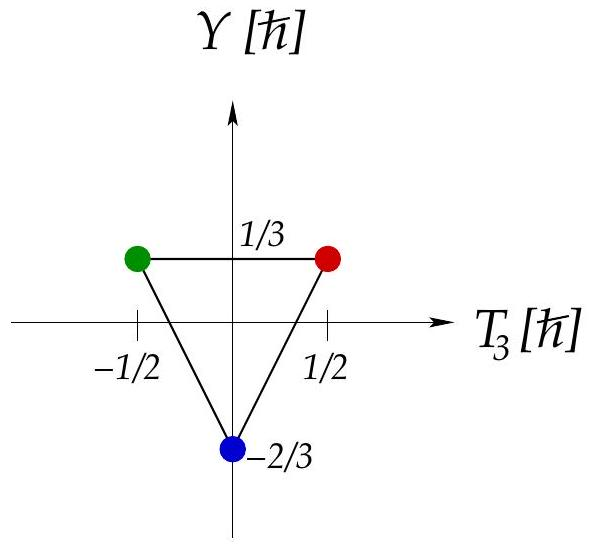
\includegraphics[scale=0.3, center]{2025_05_20_8618f55a41bfe980b4b2g-61}

The colors are assigned as follows to eigenstates $\left|T_{3} Y\right\rangle$ of "color spin" $T_{3}$ and "color hypercharge" $Y$ :

$$
\begin{aligned}
|r\rangle \equiv \mid \text { "red" }\rangle & \equiv\left|\frac{1}{2} \frac{1}{3}\right\rangle \\
|g\rangle \equiv \mid \text { "green" }\rangle & \equiv\left|-\frac{1}{2} \frac{1}{3}\right\rangle \\
|b\rangle \equiv \mid \text { "blue" }\rangle & \equiv\left|0-\frac{2}{3}\right\rangle
\end{aligned}
$$

Anti-quarks differ from quarks in all charge quantum numbers, and thus also in color. Therefore, anti-quarks occupy states of the anti-triplet,

\section{Yh}
\begin{center}
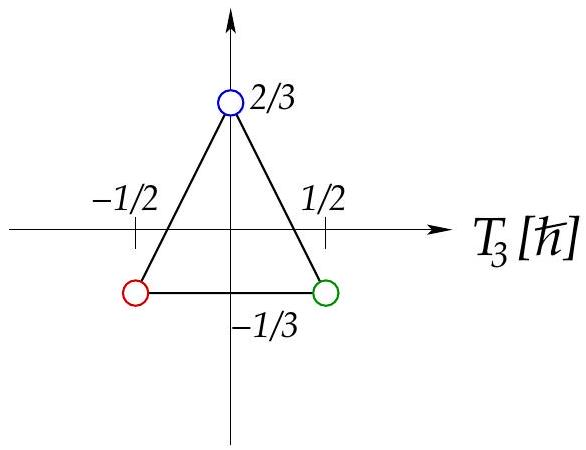
\includegraphics[scale=0.3]{2025_05_20_8618f55a41bfe980b4b2g-62}
\end{center}

The assignment of colors to $\left|T_{3} Y\right\rangle$ eigenstates is the following:

$$
\begin{aligned}
|\bar{r}\rangle \equiv \mid \text { "anti-red" }\rangle & \equiv\left|-\frac{1}{2}-\frac{1}{3}\right\rangle \\
|\bar{g}\rangle \equiv \mid \text { "anti-green" }\rangle & \equiv\left|\frac{1}{2}-\frac{1}{3}\right\rangle \\
|\bar{b}\rangle \equiv \mid \text { "anti-blue" }\rangle & \equiv\left|0 \frac{2}{3}\right\rangle
\end{aligned}
$$

The eight gluons occupy states of the adjoint representation, the octet. Since the octet can be generated by coupling a triplet and an anti-triplet, cf. Eq. (4.50), one can imagine gluons to carry combinations of colors and anti-colors.\\
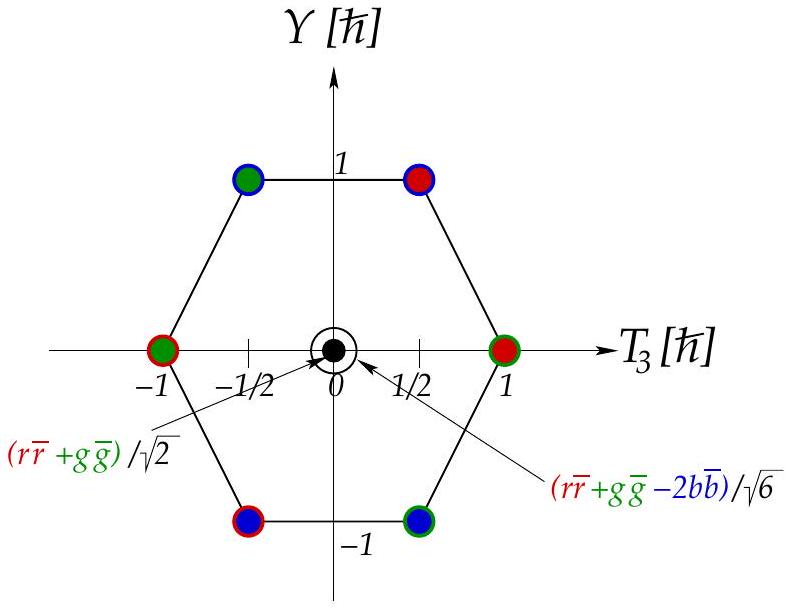
\includegraphics[scale=0.3, center]{2025_05_20_8618f55a41bfe980b4b2g-62(1)}

A peculiarity of QCD is the so-called color confinement: particles which are subject to the strong interaction, so-called hadrons, appear in Nature always as singlet ("white" objects) of the ( $S U\left(N_{c}\right), \cdot$ ) color symmetry, color-charged objects such as quarks and gluons are never observed in isolation. The confinement of color charges is an experimentally observed fact, but so far could not been shown rigorously on the basis of the theory of QCD.

The fact that hadrons are always color-singlets means that they must consist of several quarks and gluons, and in particular of such couplings between these particles which allow a singlet, e.g. as in Eqs. (4.50) and (4.52). Color-singlets which consist of a quark and an anti-quark are called mesons, color-singlets which consist of three (anti-)quarks are called (anti-)baryons. We will discuss concrete examples in the next sections, but first we discuss another symmetry of QCD, the so-called flavor symmetry.

\section{SU(N) flavor symmetry}
In the case of vanishing mass, left- and right-handed Dirac fields,

$$
\psi_{r, \ell} \equiv \mathcal{P}_{r, \ell} \psi \equiv \frac{1 \pm \gamma_{5}}{2} \psi, \quad \bar{\psi}_{r, \ell} \equiv \bar{\psi} \mathcal{P}_{\ell, r} \equiv \bar{\psi} \frac{1 \mp \gamma_{5}}{2},
$$

where $\gamma_{5}=i \gamma^{0} \gamma^{1} \gamma^{2} \gamma^{3}$, decouple in the Dirac Lagrangian,

$$
\bar{\psi} i \not \partial \psi=\bar{\psi}_{r} i \not \partial \psi_{r}+\bar{\psi}_{\ell} i \not \partial \psi_{\ell} .
$$

(In order to show this, use $\left\{\gamma_{5}, \gamma^{\mu}\right\}=0$, as well as the projector properties $\mathcal{P}_{r, \ell}^{2}=$ $\mathcal{P}_{r, \ell}, \mathcal{P}_{r} \mathcal{P}_{\ell}=\mathcal{P}_{\ell} \mathcal{P}_{r}=0, \mathcal{P}_{r}+\mathcal{P}_{\ell}=\mathbf{1}_{4}$.) This also holds for the QCD Lagrangian (5.6), which is then invariant under global unitary transformations of right- and left-handed quark fields,

$$
\begin{aligned}
\Psi_{r, \ell} & \longrightarrow \Psi_{r, \ell}^{\prime}=\hat{U}_{r, \ell} \Psi_{r, \ell} \\
\hat{U}_{r, \ell} & =\exp \left(-i \alpha_{r, \ell}^{a} \hat{T}_{a}\right) \in U\left(N_{f}\right)_{r, \ell}, \quad \alpha_{r, \ell}^{a}=\text { const. }, \quad a=0, \ldots, N_{f}^{2}-1
\end{aligned}
$$

Since one can transform right- and left-handed fields separately, the full symmetry group is $\left(U\left(N_{f}\right)_{r} \times U\left(N_{f}\right)_{\ell}, \cdot\right)$, the so-called chiral symmetry of QCD.

A mass term explicitly breaks this symmetry, as one readily confirms,

$$
\bar{\psi} m \psi=\bar{\psi}_{\ell} m \psi_{r}+\bar{\psi}_{r} m \psi_{\ell}
$$

This term is only symmetric under those chiral transformations which fulfill $\hat{U}_{\ell}^{\dagger}=\hat{U}_{\ell}^{-1}=$ $\hat{U}_{r}^{-1}$, or $\alpha_{r}^{a}=\alpha_{\ell}^{a}$. This is the symmetry of vector transformations $V=r+\ell$,

$$
\hat{U}_{V}=\exp \left(-i \alpha_{V}^{a} \hat{T}_{a}\right) \in U\left(N_{f}\right)_{V}, \quad \alpha_{V}^{a} \equiv \alpha_{r+\ell}^{a}=\alpha_{r}^{a}+\alpha_{\ell}^{a}
$$

which forms the diagonal subgroup $\left(U\left(N_{f}\right)_{V}, \cdot\right.$ ) of the chiral symmetry group ( $U\left(N_{f}\right)_{r} \times$ $U\left(N_{f}\right)_{\ell}, \cdot$ ). On the other hand, the symmetry of axial-vector transformations $A=$ $r-\ell$,

$$
\hat{U}_{A}=\exp \left(-i \gamma_{5} \alpha_{A}^{a} \hat{T}_{a}\right) \in U\left(N_{f}\right)_{A}, \quad \alpha_{A}^{a} \equiv \alpha_{r-\ell}^{a}=\alpha_{r}^{a}-\alpha_{\ell}^{a},
$$

is explicitly broken. (There is no such symmetry, since the mass term requires $\alpha_{r}^{a}=\alpha_{\ell}^{a}$, which means that $\alpha_{A}^{a} \equiv 0$.)

The individual quark masses are non-zero,

$$
\begin{array}{ll}
m_{u} \simeq 2.3 \mathrm{MeV}, & m_{d} \simeq 4.8 \mathrm{MeV}, \\
m_{s} \simeq 95 \mathrm{MeV}, & m_{c} \simeq 1.275 \mathrm{GeV}, \\
m_{b} \simeq 4.18 \mathrm{GeV}, & m_{t} \simeq 173.21 \mathrm{GeV},
\end{array}
$$

consequently, the chiral symmetry of QCD is explicitly broken. If all quark masses were equal, then the residual symmetry of QCD would be that of the vector transformations, $\left(U\left(N_{f}\right)_{V}, \cdot\right.$ ). Since $U(N)=S U(N) \otimes U(1)$, cf. Exercises 3 and 4, and the $U(1)_{V}$ symmetry represents according to Noether's theorem simply the (trivial) conservation of quark\\
number, one usually considers the group $\left(S U\left(N_{f}\right), \cdot\right)$ of special unitary vector transformations, or short, the ( $\boldsymbol{S U}\left(\boldsymbol{N}_{f}\right), \cdot$ ) flavor symmetry.

This symmetry is broken because the quark masses (5.27) are all of different value. However, for some quark flavors the breaking is less strong than for others. For instance, the mass difference between up and down quark is, in comparison to a typical hadronic mass scale of $M_{h} \sim 1 \mathrm{GeV}$, vanishingly small. This results in an approximate ( $S U(2), \cdot$ ) flavor symmetry, the so-called isospin symmetry of QCD and thus of the strong interaction, which will be discussed in the next section. Moreover, also the mass difference between strange and up or down quark is, on a hadronic mass scale, small, so that one can assume to good approximation also an approximate $(S U(3), \cdot)$ flavor symmetry of the strong interaction. This will be discussed in the next-to-next section. More strongly broken is the $(S U(4), \cdot)$ flavor symmetry, which also takes into account the charm quark. It is nevertheless reasonable to also consider this symmetry in order to classify hadrons with the quantum number charm, which will be done at the end of this chapter.

\subsection{Isospin symmetry}
The masses of up and down quark are, in comparison to a hadronic mass scale $M_{h} \sim 1$ GeV, almost of equal magnitude (and also vanishingly small),

$$
m_{u} \simeq 2.3 \mathrm{MeV}<m_{d} \simeq 4.8 \mathrm{MeV} \ll M_{h} \sim 1 \mathrm{GeV}
$$

Therefore, one can to good approximation assume that QCD possesses an ( $S U(2), \cdot$ ) flavor symmetry. (Since the quark masses are vanishingly small compared to $M_{h}$, one may think that the symmetry group is actually larger, namely that of chiral symmetry for $N_{f}=2$ massless flavors, $U(2)_{r} \times U(2)_{\ell}$. This is, however, not true because of spontaneous breaking of chiral symmetry by a non-vanishing quark condensate $\langle\bar{\Psi} \Psi\rangle \neq 0$.)

We write

$$
\bar{m} \equiv \frac{1}{2}\left(m_{u}+m_{d}\right), \quad \delta m \equiv m_{d}-m_{u}
$$

so that

$$
m_{u}=\bar{m}-\frac{\delta m}{2}, \quad m_{d}=\bar{m}+\frac{\delta m}{2}
$$

and neglect the mass difference $\delta m$ in the following. Then, the $(S U(2), \cdot)$ flavor symmetry of QCD is even an exact symmetry. Up and down quark form an ( $\boldsymbol{S} \boldsymbol{U}(\mathbf{2}), \cdot)$ doublet, [2],\\
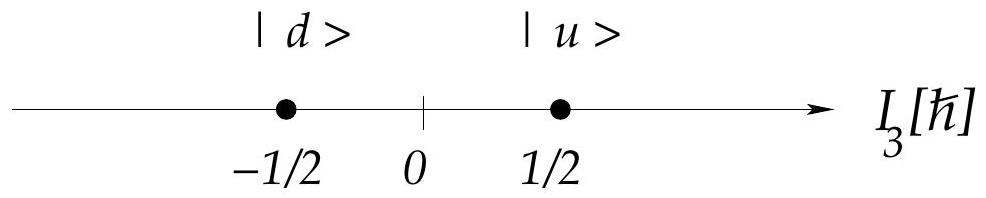
\includegraphics[scale=0.3, center]{2025_05_20_8618f55a41bfe980b4b2g-64}

If we denote the states with $\left|I I_{3}\right\rangle$, we have

$$
\begin{aligned}
|u\rangle & \equiv|" u p "\rangle=\left|\frac{1}{2} \frac{1}{2}\right\rangle \\
|d\rangle & \equiv \mid " \text { down" }\rangle=\left|\frac{1}{2}-\frac{1}{2}\right\rangle
\end{aligned}
$$

The corresponding anti-doublet $[\overline{2}]$ consists of the corresponding antiparticles, the antiup $\bar{u}$ and anti-down quark $\bar{d}$. Formally, it has the same shape as the doublet,\\
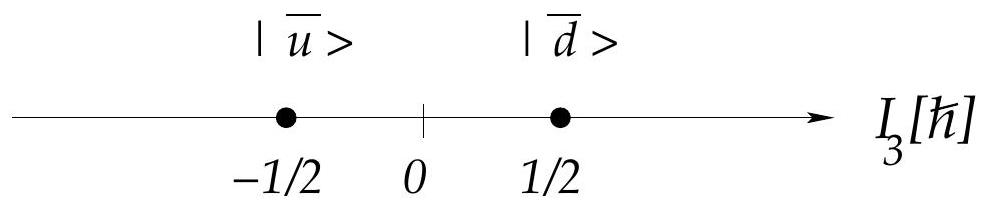
\includegraphics[scale=0.3, center]{2025_05_20_8618f55a41bfe980b4b2g-65}

The assignment of states reads

$$
\begin{aligned}
|\bar{u}\rangle & \equiv \mid \text { "anti-up" }\rangle=\left|\frac{1}{2}-\frac{1}{2}\right\rangle \\
|\bar{d}\rangle & \equiv \mid \text { "anti-down" }\rangle=\left|\frac{1}{2} \frac{1}{2}\right\rangle
\end{aligned}
$$

Because of the formal similarity with [2] the coupling rules for the anti-doublet are identical with those of the doublet, i.e., in analogy to Eq. (4.46) we have

$$
[2] \otimes[\overline{2}]=[1] \oplus[3]
$$

Because of the ( $S U(2), \cdot$ ) symmetry, all hadrons which are composed of up and down quarks (or the respective anti-quarks) must also fall into ( $S U(2), \cdot$ ) multiplets. The assignment follows the coupling rules for $(S U(2), \cdot)$, which we have discussed in Sec. 4.5. Since the eigenvalues of the Hamilton operator $\hat{H}\left(\hat{C}_{1}\right)$ are degenerate on a multiplet, all hadrons of a given multiplet must possess the same mass, if the ( $S U(2), \cdot$ ) flavor symmetry is exact. Therefore, the ( $S U(2), \cdot$ ) flavor symmetry is also called isobaric spin symmetry, or short isospin symmetry (greek: 'íoos $\beta \alpha p u s=$ equally heavy). This is the origin of the labels $I$ and $I_{3}$ for magnitude and 3-component of the isospin.

Mesons are colorless quark-anti-quark states. The possible ( $S U(2), \cdot$ ) flavor multiplets can be determined from Eq. (5.30), i.e., there is a flavor singlet and a flavor triplet. Considering the respective Clebsch-Gordan coefficients one obtains\\
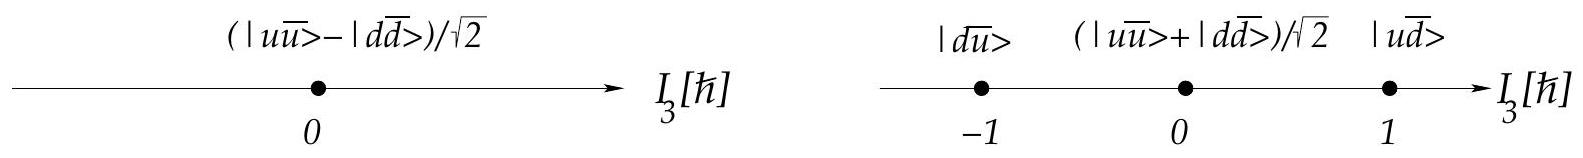
\includegraphics[scale=0.3, center]{2025_05_20_8618f55a41bfe980b4b2g-65(1)}

There are, however, different kinds of mesons with the same flavor content, but different behavior under Lorentz transformations, i.e., they differ in their spin $J$. The usual classification follows according to the isospin $I$ of the meson, and then according to spin $J$, parity $P$, and charge conjugation $C$, with the notation $J^{P C}$. Some of the $N_{f}=2$ mesons are listed in Tab. 5.1.

The state of the triplet differ in their electric charge, which can be calculated according to the formula

$$
Q=e I_{3} \quad(\text { mesons })
$$

As one observes, the isospin symmetry is nearly exact, only the different states of the pion triplet differ slightly in their masses,

$$
\delta m_{\pi}=m_{\pi^{ \pm}}-m_{\pi^{0}}=4.59358 \mathrm{MeV} \ll m_{\pi^{ \pm}}, m_{\pi^{0}}
$$

\begin{center}
\begin{tabular}{|l|l|l|l|}
\hline
Mesons & [1] ( $I=0$ ) & \multicolumn{2}{|c|}{[3] ( $I=1$ )} \\
\hline
Scalars ( $J^{P C}=0^{++}$) & $f_{0}(1370)$ & $a_{0}^{ \pm}(1450)$ & $a_{0}^{0}(1450)$ \\
\hline
Mass [MeV] & $1350 \pm 150$ & \multicolumn{2}{|c|}{$1474 \pm 19$} \\
\hline
Pseudoscalars ( $J^{P C}=0^{-+}$) & $\eta$ & $\pi^{ \pm}$ & $\pi^{0}$ \\
\hline
Mass [MeV] & $547.862 \pm 0.018$ & $139.57018 \pm 0.00035$ & $134.9766 \pm 0.0006$ \\
\hline
Vectors ( $J^{P C}=1^{--}$) & $\omega$ & $\rho^{ \pm}$ & $\rho^{0}$ \\
\hline
Mass [MeV] & $782.65 \pm 0.12$ & \multicolumn{2}{|c|}{$775.26 \pm 0.25$} \\
\hline
Axial-vectors ( $J^{P C}=1^{++}$) & $f_{1}(1285)$ & $a_{1}^{ \pm}(1260)$ & $a_{1}^{0}(1260)$ \\
\hline
Masse [MeV] & $1281.9 \pm 0.5$ & \multicolumn{2}{|c|}{$1230 \pm 40$} \\
\hline
\end{tabular}
\end{center}

Table 5.1: Mesons which consist of a quark and an anti-quark.

Baryons are colorless states composed of three quarks. The possible flavor multiplets can be determined from

$$
[2] \otimes[2] \otimes[2]=[2] \otimes([1] \oplus[3])=[2] \oplus[2] \oplus[4]
$$

One of the doublets is the nucleon doublet, consisting of proton and neutron:\\
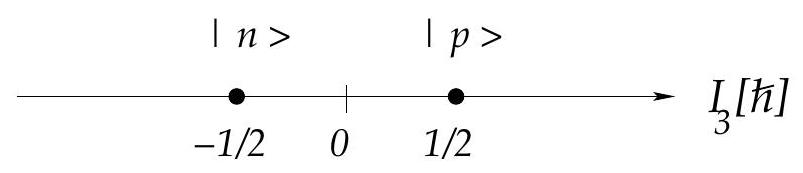
\includegraphics[scale=0.3, center]{2025_05_20_8618f55a41bfe980b4b2g-66(1)}

Taking into account the Clebsch-Gordan coefficients, the flavor content of proton and neutron is

$$
\begin{aligned}
|p\rangle & \equiv \mid \text { "proton" }\rangle=\left|\frac{1}{2} \frac{1}{2}\right\rangle=\frac{1}{\sqrt{6}}(|u u d\rangle+|u d u\rangle-2|d u u\rangle) \\
|n\rangle & \equiv \mid \text { "neutron" }\rangle=\left|\frac{1}{2}-\frac{1}{2}\right\rangle=\frac{1}{\sqrt{6}}(2|u d d\rangle-|d u d\rangle-|d d u\rangle)
\end{aligned}
$$

The quantum numbers of the nucleon doublet read $I\left(J^{P}\right)=\frac{1}{2}\left(\frac{1}{2}^{+}\right)$and the masses are

$$
m_{n}=939.565379 \pm 0.000021 \mathrm{MeV}, \quad m_{p}=938.272046 \pm 0.000021 \mathrm{MeV}
$$

so that the mass difference (and thus isospin violation) is again small compared to the absolute magnitude of the nucleon masses,

$$
\delta m_{N}=m_{n}-m_{p}=1.293333 \mathrm{MeV} \ll m_{n}, m_{p}
$$

The quadruplet in Eq. (5.32) is that of the so-called Delta resonances:\\
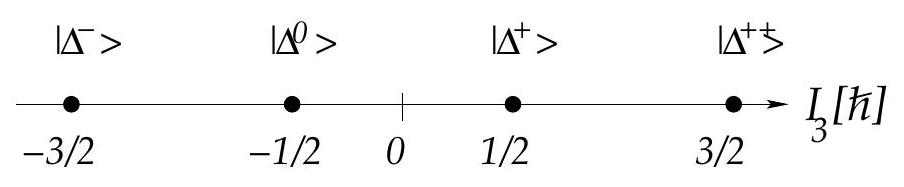
\includegraphics[scale=0.3, center]{2025_05_20_8618f55a41bfe980b4b2g-66}

Taking into account the Clebsch-Gordan coefficients, the flavor content of the $\Delta$ resonances reads

$$
\begin{aligned}
\left|\Delta^{++}\right\rangle & =\left|\frac{3}{2} \frac{3}{2}\right\rangle=|u u u\rangle \\
\left|\Delta^{+}\right\rangle & =\left|\frac{3}{2} \frac{1}{2}\right\rangle=\frac{1}{\sqrt{3}}(|u u d\rangle+|u d u\rangle+|d u u\rangle) \\
\left|\Delta^{0}\right\rangle & =\left|\frac{3}{2}-\frac{1}{2}\right\rangle=\frac{1}{\sqrt{3}}(|u d d\rangle+|d u d\rangle+|d d u\rangle) \\
\left|\Delta^{-}\right\rangle & =\left|\frac{3}{2}-\frac{3}{2}\right\rangle=|d d d\rangle
\end{aligned}
$$

The quantum numbers of the $\Delta$ quadruplet are $I\left(J^{P}\right)=\frac{3}{2}\left(\frac{3}{2}\right)^{+}$and the mass is $m_{\Delta}=1232$ MeV .

In order to compute the electric charge of the baryons, Eq. 5.31 needs to be modified:

$$
Q=e\left(I_{3}+\frac{1}{2}\right) \quad \text { (baryons) }
$$

\subsection{Strangeness and SU(3) flavor symmetry}
The difference between the masses of up, down, and strange quarks is, in comparison to a typical hadronic mass scale $M_{h} \sim 1 \mathrm{GeV}$, still relatively small,

$$
\begin{aligned}
& \delta m_{u d}=m_{d}-m_{u} \simeq 2.5 \mathrm{MeV} \\
< & \delta m_{d s}=m_{s}-m_{d} \simeq 90 \mathrm{MeV} \\
\simeq & \delta m_{u s}=m_{s}-m_{u} \simeq 92.7 \mathrm{MeV} \\
\ll & M_{h} \sim 1 \mathrm{GeV},
\end{aligned}
$$

so that one can speak of an approximate $(S U(3), \cdot)$ flavor symmetry of the strong interaction. In the following, we first neglect the mass differences $\delta m_{u d}, \delta m_{d s}$, and $\delta m_{u s}$ and assume an exact ( $S U(3), \cdot$ ) flavor symmetry.

Then, the three quark flavors form an ( $S U(3), \cdot$ ) triplet:

\section{Yh}
\begin{center}
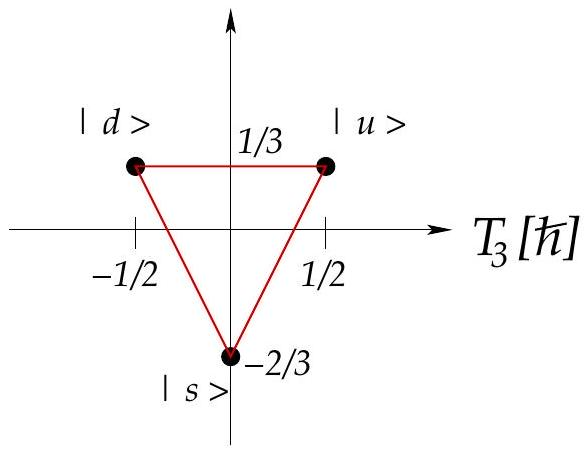
\includegraphics[scale=0.3]{2025_05_20_8618f55a41bfe980b4b2g-67}
\end{center}

The role of the 3 -component of isospin from the preceding section is now assumed by $T_{3}$. The assignment of states is

$$
\begin{aligned}
|u\rangle \equiv \mid " \text { up" }\rangle & \equiv\left|\frac{1}{2} \frac{1}{3}\right\rangle \\
|d\rangle \equiv \mid \text { "down" }\rangle & \equiv\left|-\frac{1}{2} \frac{1}{3}\right\rangle \\
|s\rangle \equiv \mid \text { "strange" }\rangle & \equiv\left|0-\frac{2}{3}\right\rangle
\end{aligned}
$$

Note the analogy to the assignment of the three colors red, green, and blue in the case of the $(S U(3), \cdot)$ color symmetry of QCD.

Anti-quarks form an anti-triplet:

$$
Y[\hbar]
$$

\begin{center}
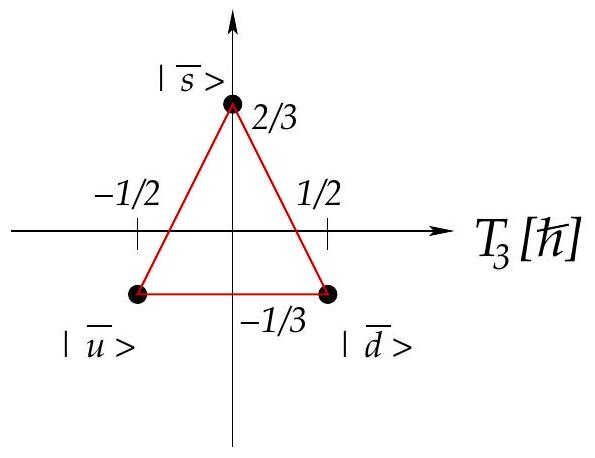
\includegraphics[scale=0.3]{2025_05_20_8618f55a41bfe980b4b2g-68}
\end{center}

The assignment of states is

$$
\begin{aligned}
|\bar{u}\rangle \equiv \mid " \text { anti-up" }\rangle & \equiv\left|-\frac{1}{2}-\frac{1}{3}\right\rangle \\
|\bar{d}\rangle \equiv \mid \text { "anti-down" }\rangle & \equiv\left|\frac{1}{2}-\frac{1}{3}\right\rangle \\
|\bar{s}\rangle \equiv \mid \text { "anti-strange" }\rangle & \equiv\left|0 \frac{2}{3}\right\rangle
\end{aligned}
$$

According to the coupling rule 4.50, mesons form a singlet and an octet:\\
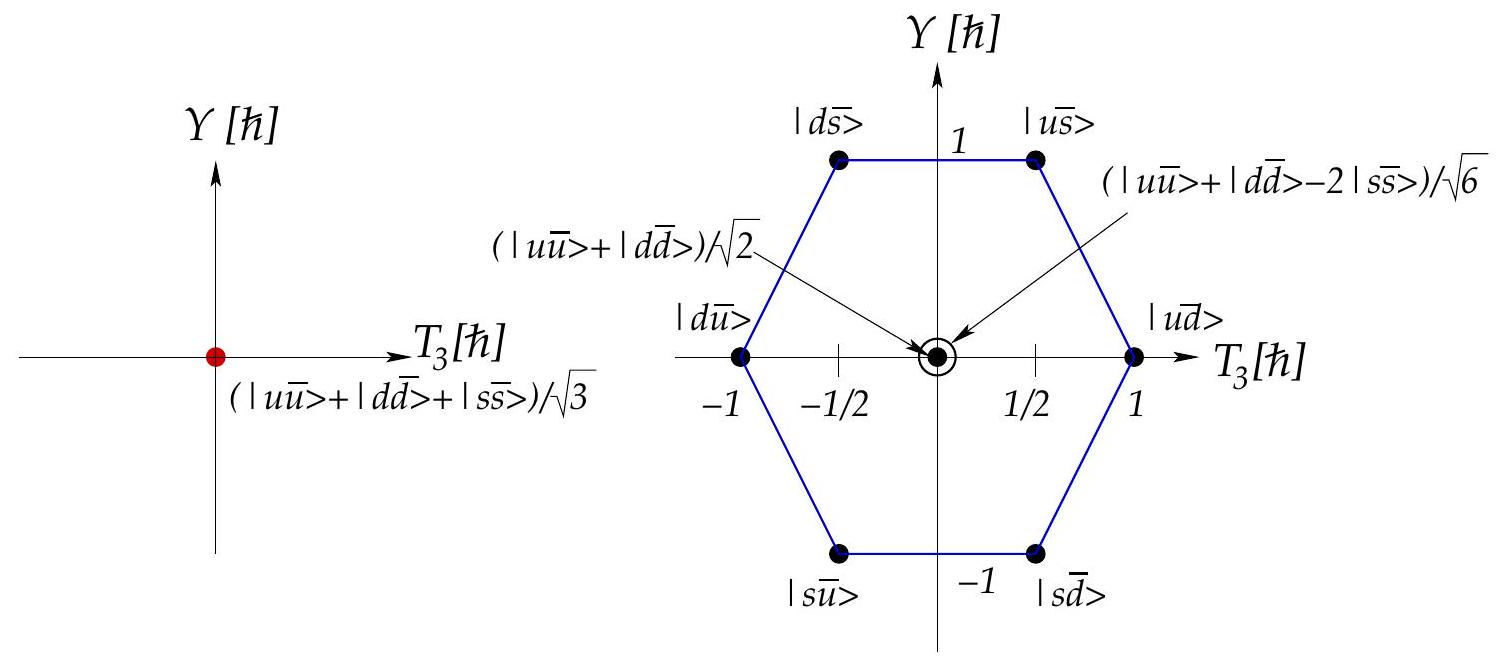
\includegraphics[scale=0.3, center]{2025_05_20_8618f55a41bfe980b4b2g-68(1)}

We distinguish\\
(i) Scalar mesons, $J^{P C}=0^{++}$:\\
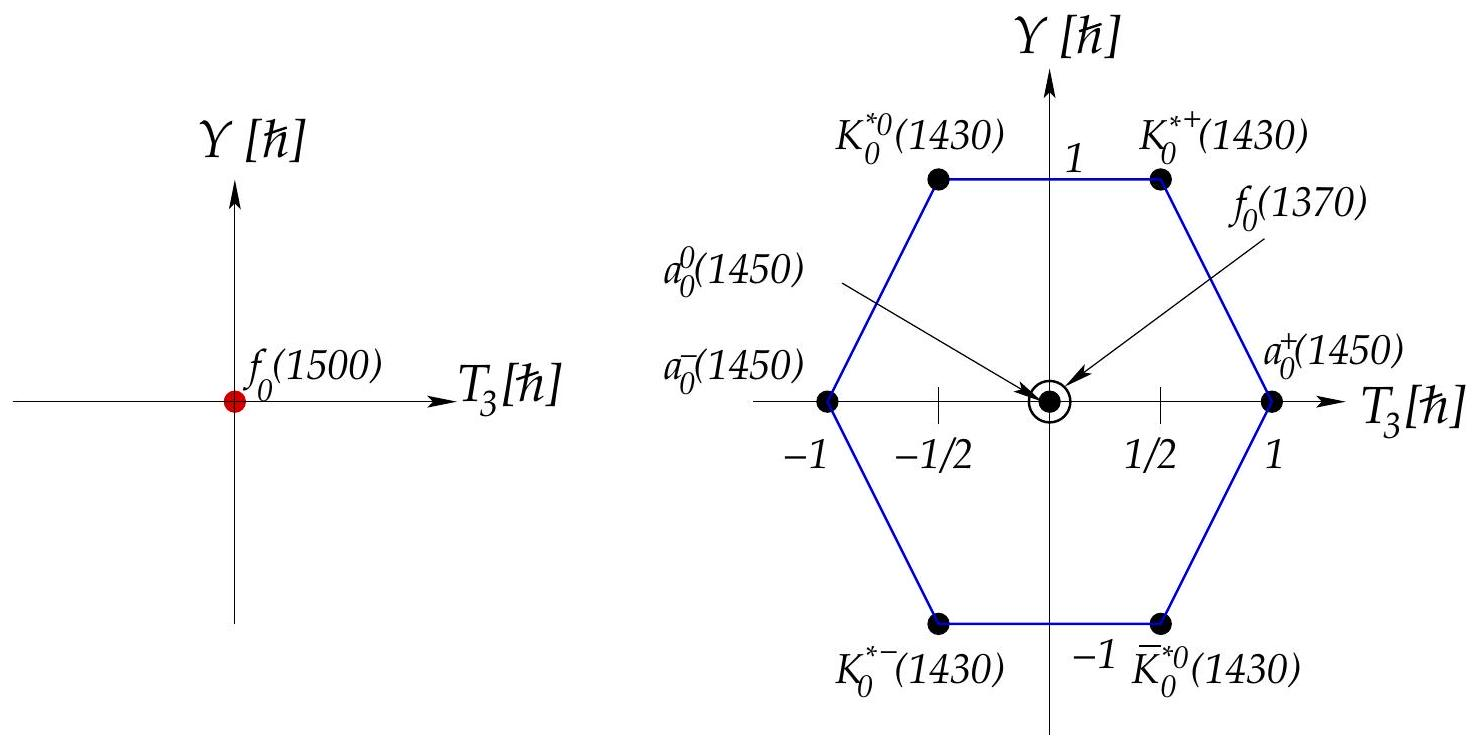
\includegraphics[scale=0.3, center]{2025_05_20_8618f55a41bfe980b4b2g-69}

As we observe, the isosinglet $f_{0}(1370)$ and the isotriplet of $a_{0}(1260)$ mesons from the $N_{f}=2$ case are parts of the octet. New as compared to the latter case are the four scalar $K_{0}^{*}$ mesons, which form two isospin doublets inside the octet. The new isoscalar $f_{0}(1500)$ meson constitutes the singlet. The masses and isospin quantum numbers of these mesons are:

$$
\begin{array}{rll}
f_{0}(1500) & : I=0, & m_{f_{0}(1500)}=1505 \pm 6 \mathrm{MeV} \\
K_{0}^{*}(1430) & : I=\frac{1}{2}, & m_{K_{0}^{*}}=1425 \pm 50 \mathrm{MeV}
\end{array}
$$

(ii) Pseudoscalar mesons, $J^{P C}=0^{-+}$:\\
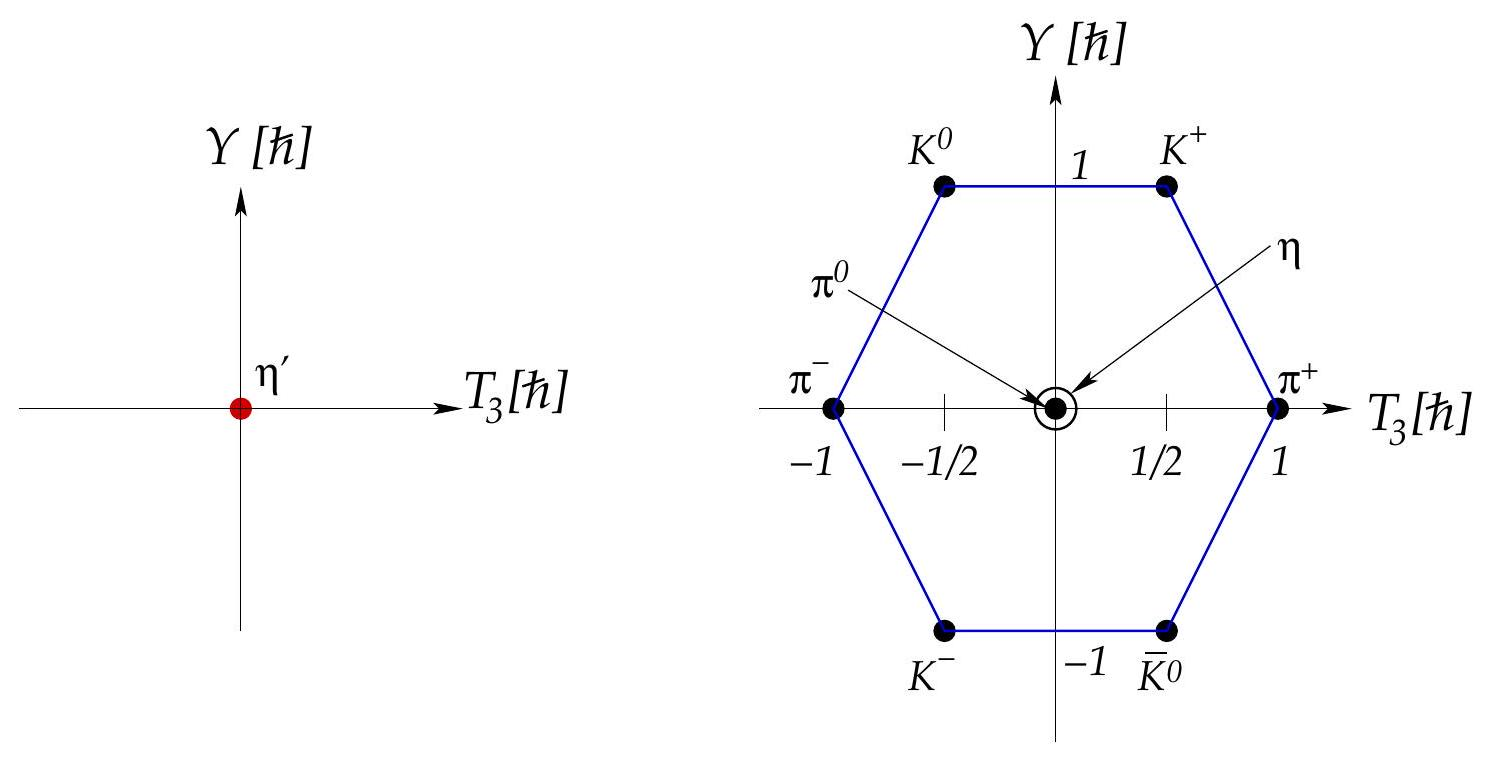
\includegraphics[scale=0.3, center]{2025_05_20_8618f55a41bfe980b4b2g-69(1)}

As we observe, the isosinglet $\eta$ and the pion isotriplet from the $N_{f}=2$ case are parts of the octet. New as compared to the latter case are the four pseudoscalar $K$ mesons, or short kaons, which form two isospin doublets inside the octet. The new isoscalar $\eta^{\prime}$ meson constitutes the singlet. The masses and isospin quantum numbers of these mesons are:


$$\begin{array}{ll}
    \eta^{\prime}: I=0, & m_{\eta^{\prime}}=957.78 \pm 0.06 \mathrm{MeV} \\
    K: I=\frac{1}{2}, & m_{K^{ \pm}}=493.677 \pm 0.016 \mathrm{MeV} \\
    & m_{K^{0}}=497.614 \pm 0.024 \mathrm{MeV}
\end{array}$$
    

(iii) Vector mesons, $J^{P C}=1^{--}$:\\
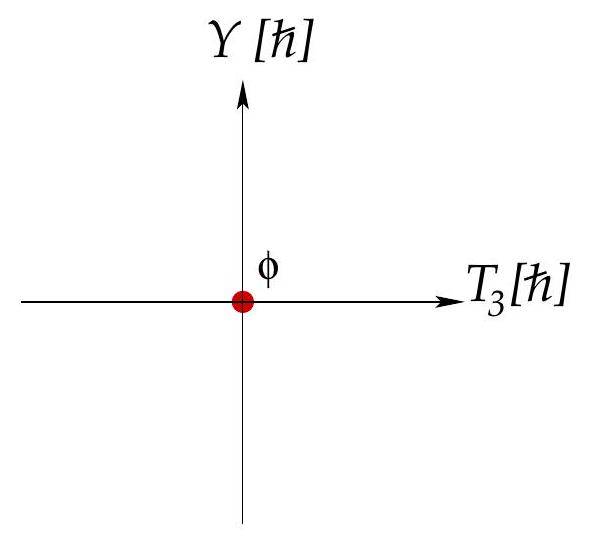
\includegraphics[scale=0.3, center]{2025_05_20_8618f55a41bfe980b4b2g-70}\\
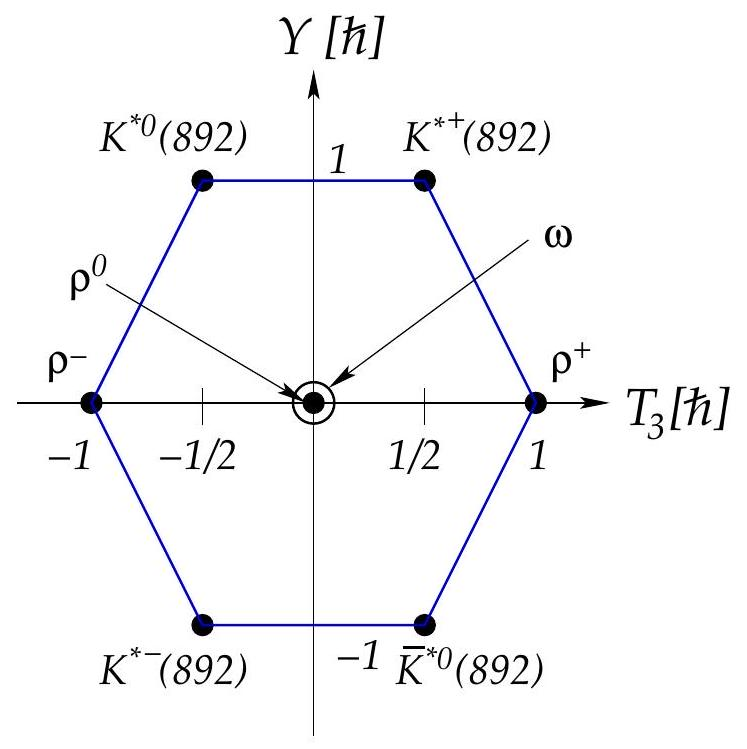
\includegraphics[scale=0.3, center]{2025_05_20_8618f55a41bfe980b4b2g-70(1)}

As we observe, the isosinglet $\omega$ and the isotriplet of the $\rho$ mesons from the $N_{f}=2$ case are parts of the octet. New as compared to the latter case are the four vector $K^{*}$ mesons, which form two isospin doublets inside the octet. The new isoscalar $\phi$ meson constitutes the singlet. The masses and isospin quantum numbers of these mesons are:

$$
\begin{array}{rll}
\phi & : I=0, & m_{\phi}=1019.461 \pm 0.019 \mathrm{MeV} \\
K^{*} & : I=\frac{1}{2}, & m_{K^{*}}=891.66 \pm 0.26 \mathrm{MeV}
\end{array}
$$

(iv) Axial-vector mesons, $J^{P C}=1^{++}$:\\
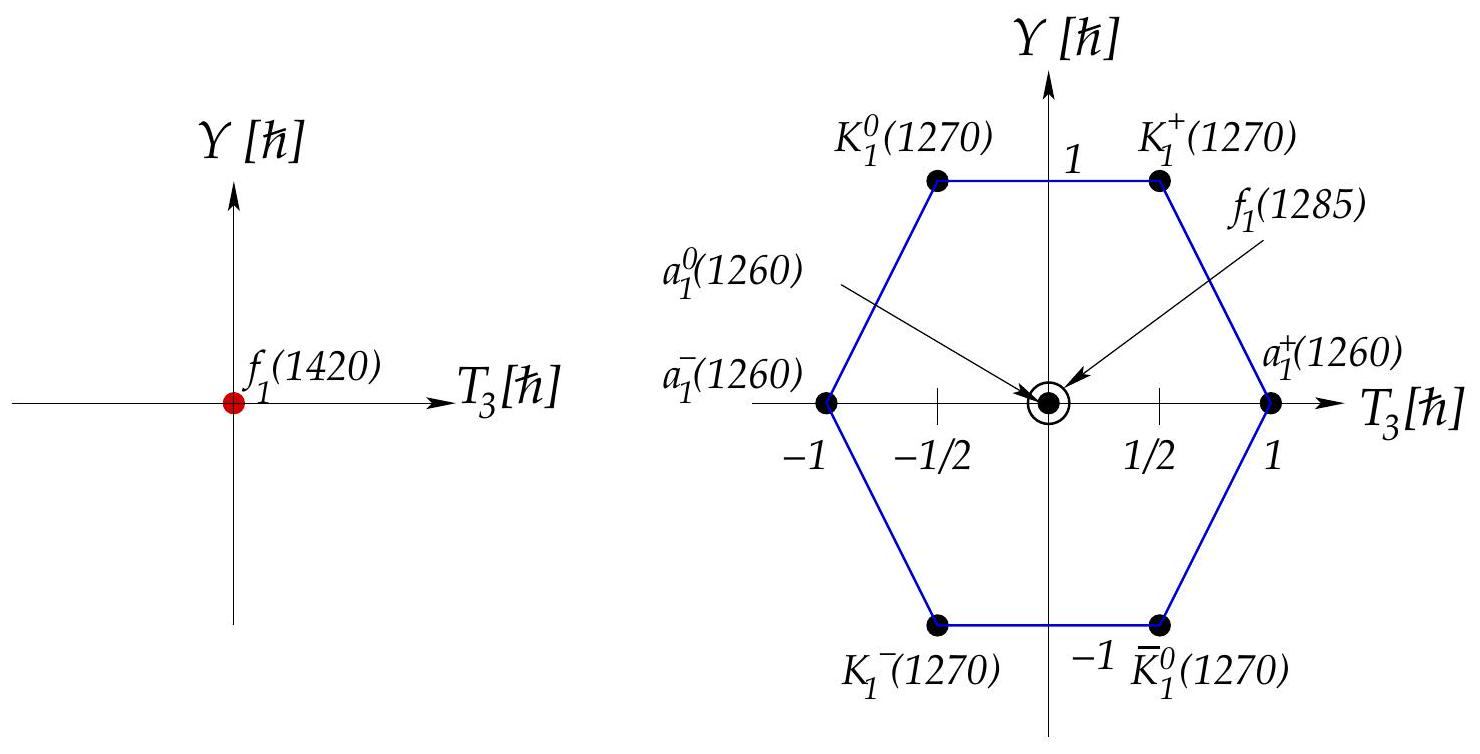
\includegraphics[scale=0.3, center]{2025_05_20_8618f55a41bfe980b4b2g-71}

The isosinglet $f_{1}(1285)$ and the isotriplet of the $a_{1}$ mesons from the case $N_{f}=2$ are parts of the octet. New as compared to the case $N_{f}=2$ are the four axial-vector $K_{1}$ mesons, which form two isospin doublets inside the octet. The new isoscalar $f_{1}(1420)$ meson constitutes the singlet. The masses and isospin quantum numbers of these mesons are:

$$
\begin{array}{rll}
f_{1}(1420) & : & I=0, \\
K_{1} & : & I=\frac{1}{2},
\end{array} \quad \begin{aligned}
& m_{f_{1}(1420)}=1426.4 \pm 0.9 \mathrm{MeV} \\
& m_{K_{1}}=1272 \pm 7 \mathrm{MeV}
\end{aligned}
$$

According to the coupling rule (4.52), baryons form a singlet, two octets, and a decuplet:\\
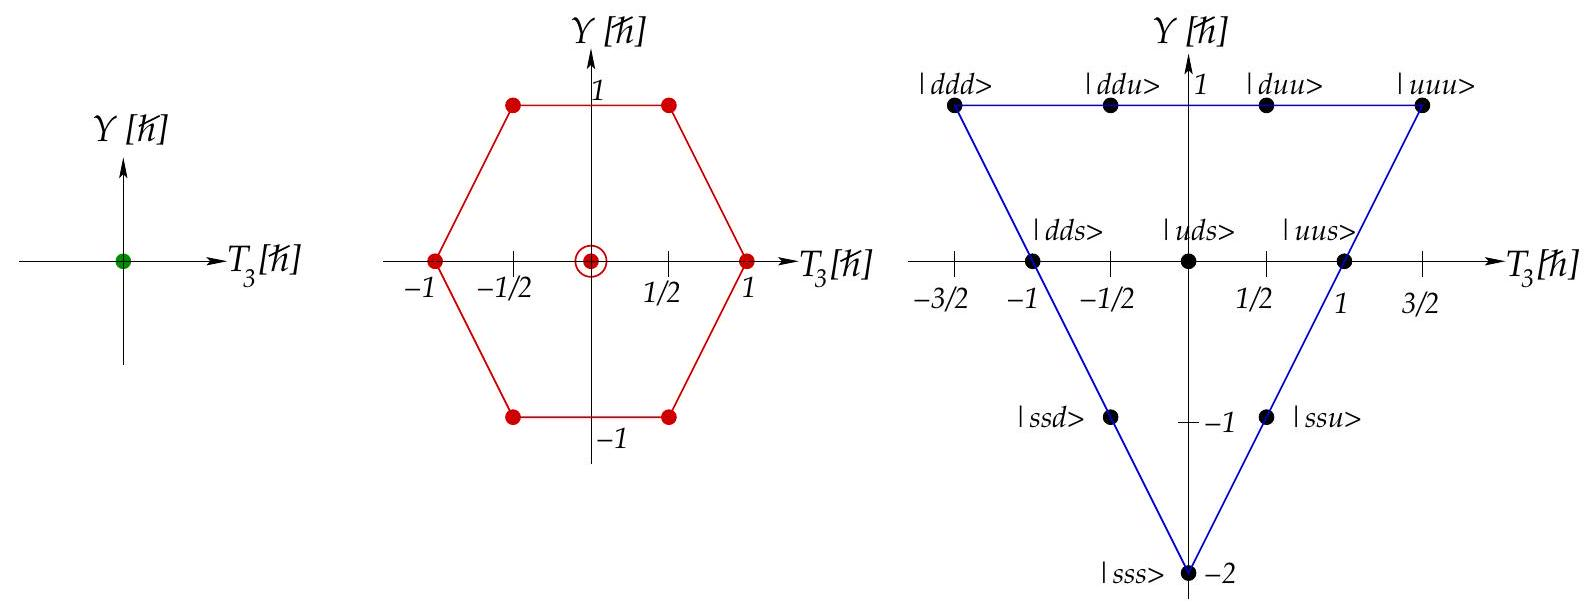
\includegraphics[scale=0.3, center]{2025_05_20_8618f55a41bfe980b4b2g-71(1)}

We only show one of the two octets, and we just indicate the flavor content of the states of the decuplet, without respecting proper symmetrization. The flavor content of the states of the singlet and of the two octets is in principle the same as that of the corresponding states of the decuplet, but the quarks appear in different combinations, corresponding to the respective symmetry of the state under exchange of particles. Due to lack of time, we cannot discuss this further at this point.

We just mention the assignment of physical baryon states to these multiplets:\\
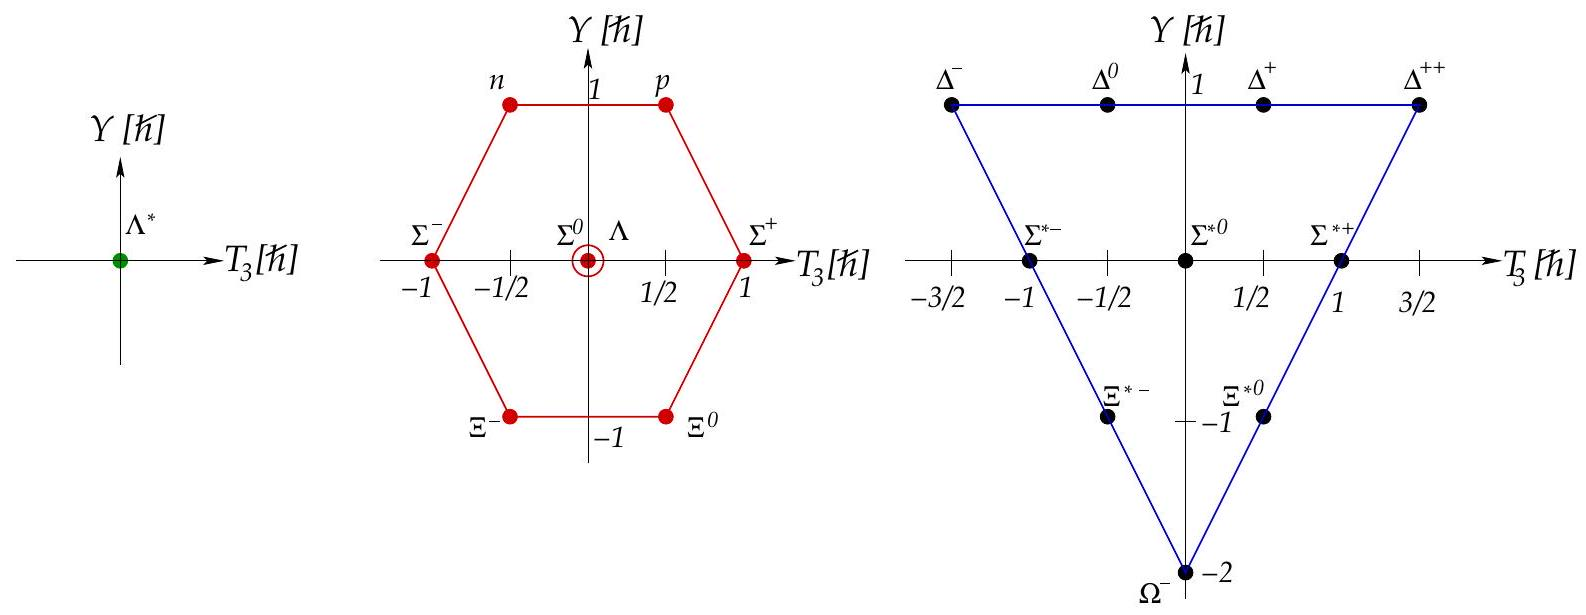
\includegraphics[scale=0.3, center]{2025_05_20_8618f55a41bfe980b4b2g-72}

We observe that the nucleon isodoublet is part of the octet and the $\Delta$ isoquadruplet is part of the decuplet. New baryon states as compared to the case $N_{f}=2$ are:

$$
\begin{array}{rll}
\Lambda & : I\left(J^{P}\right)=0\left(\frac{1}{2}^{+}\right), & m_{\Lambda}=1115.683 \pm 0.006 \mathrm{MeV} \\
\Sigma^{+} & : I\left(J^{P}\right)=1\left(\frac{1}{2}^{+}\right), & m_{\Sigma^{+}}=1189.37 \pm 0.07 \mathrm{MeV} \\
\Sigma^{0} & : I\left(J^{P}\right)=1\left(\frac{1}{2}^{+}\right), & m_{\Sigma^{0}}=1192.642 \pm 0.024 \mathrm{MeV} \\
\Sigma^{-} & : I\left(J^{P}\right)=1\left(\frac{1}{2}^{+}\right), & m_{\Sigma^{-}}=1197.449 \pm 0.030 \mathrm{MeV} \\
\Xi^{0} & : I\left(J^{P}\right)=\frac{1}{2}\left(\frac{1}{2}^{+}\right), & m_{\Xi^{0}}=1314.86 \pm 0.20 \mathrm{MeV} \\
\Xi^{-} & : I\left(J^{P}\right)=\frac{1}{2}\left(\frac{1}{2}^{+}\right), & m_{\Xi^{-}}=1321.71 \pm 0.07 \mathrm{MeV} \\
\Lambda^{*} & : I\left(J^{P}\right)=0\left(\frac{1}{2}^{+}\right), & m_{\Lambda^{*}}=1630 \pm 70 \mathrm{MeV} \\
\Sigma^{*+} & : I\left(J^{P}\right)=1\left(\frac{3}{2}^{+}\right), & m_{\Sigma^{*+}}=1382.80 \pm 0.35 \mathrm{MeV} \\
\Sigma^{* 0} & : I\left(J^{P}\right)=1\left(\frac{3}{2}^{+}\right), & m_{\Sigma^{* 0}}=1383.7 \pm 1.0 \mathrm{MeV} \\
\Sigma^{*-} & : I\left(J^{P}\right)=1\left(\frac{3}{2}^{+}\right), & m_{\Sigma^{*-}}=1387.2 \pm 0.5 \mathrm{MeV} \\
\Xi^{* 0} & : I\left(J^{P}\right)=\frac{1}{2}\left(\frac{3}{2}^{+}\right), & m_{\Xi^{* 0}}=1531.80 \pm 0.32 \mathrm{MeV} \\
\Xi^{*-} & : I\left(J^{P}\right)=\frac{1}{2}\left(\frac{3}{2}^{+}\right), & m_{\Xi^{*-}}=1535.0 \pm 0.6 \mathrm{MeV} \\
\Omega^{-} & \left.: I\left(J^{P}\right)=0\left(\frac{3}{2}\right)^{+}\right), & m_{\Omega^{-}}=1672.45 \pm 0.29 \mathrm{MeV}
\end{array}
$$

The corresponding anti-baryons are members of a singlet, two anti-octets (which have, however, the same shape as the octets), and an anti-decuplet. Besides these baryons, there is a multitude of further excited states, as well as such of negative parity. Because of identical flavor content, also these states must be members of a singlet, two octets, and a decuplet. Further details can be found in the compilation of the Particle Data Group [8].

With the help of the hypercharge, the empirically found charge formulas (5.31) and (5.33) can now be generalized to all ( $\operatorname{SU}(3), \cdot$ ) multiplets,

$$
Q=e\left(T_{3}+\frac{1}{2} Y\right)
$$

This is the so-called Gell-Mann-Nishijima formula. One readily checks that it holds for meson as well as for baryon multiplets. If it is valid for all ( $S U(3), \cdot$ ) multiplets,\\
it should also apply to the triplet. Thus it follows that

$$
\begin{aligned}
Q_{u} & =e\left(\frac{1}{2}+\frac{1}{2} \cdot \frac{1}{3}\right)=\frac{2}{3} e, \\
Q_{d} & =e\left(-\frac{1}{2}+\frac{1}{2} \cdot \frac{1}{3}\right)=-\frac{1}{3} e, \\
Q_{s} & =e\left(0-\frac{1}{2} \cdot \frac{2}{3}\right)=-\frac{1}{3} e .
\end{aligned}
$$

Murray Gell-Mann was the first to systematically assign hadrons to ( $\operatorname{SU}(3), \cdot$ ) flavor multiplets and interpret them as quark-anti-quark (mesons) or three-quark states (baryons), respectively. His realization culminated in postulating the existence of quarks as "building blocks" of the hadrons.

If the ( $S U(3), \cdot$ ) flavor symmetry were exact, all hadrons of a given multiplet should be degenerate in mass. This is obviously not the case. However, we observe that the isospin symmetry, i.e., the mass degeneracy inside an isospin multiplet as part of an $(S U(3), \cdot)$ flavor multiplet still holds to very good approximation. Deviations are of the order of the mass difference between up and down quark. Quite analogously, the violation of ( $\operatorname{SU}(3), \cdot$ ) flavor symmetry, i.e., the mass difference between various isospin multiplets inside an ( $\operatorname{SU}(3), \cdot$ ) flavor multiplet, is of the order of the mass difference between up or down and strange quark. For instance, for the baryons we have

$$
\begin{aligned}
m_{\Lambda}-m_{N} & \simeq 176.76 \mathrm{MeV} \\
m_{\Xi}-m_{\Lambda} & \simeq 202.60 \mathrm{MeV} \\
m_{\Sigma^{*}}-m_{\Delta} & \simeq 152.57 \mathrm{MeV} \\
m_{\Xi^{*}}-m_{\Sigma^{*}} & \simeq 148.83 \mathrm{MeV} \\
m_{\Omega}-m_{\Xi^{*}} & \simeq 139.05 \mathrm{MeV}
\end{aligned}
$$

where we have assumed averaged values inside an isospin multiplet. Obviously, the mass of the baryons grows proportional to the number of strange quarks contained in them, by an amount of the order of the strange quark mass.

This observation can also be expressed in terms of an empirical formula. To this end, we write the Hamilton operator of QCD symbolically in the form

$$
\hat{H}_{\mathrm{QCD}}=\hat{H}_{S U(3)}+\hat{H}_{\mathrm{FSB}}
$$

where the first part, $\hat{H}_{S U(3)}$, is assumed to be invariant under $(S U(3), \cdot)$ flavor transformations, while the second part, $\hat{H}_{\mathrm{FSB}}$, breaks ( $\operatorname{SU}(3), \cdot$ ) flavor symmetry explicitly. If $\hat{H}_{\mathrm{FSB}}=0$, all hadrons of an ( $\operatorname{SU}(3), \cdot$ ) flavor multiplet must have identical masses, since $\hat{H}_{S U(3)}$ can only depend on the Casimir operators $\hat{C}_{1}, \hat{C}_{2}$ of $(S U(3), \cdot)$, which assume the same eigenvalues on any given multiplet. In the following, the eigenvalue of $\hat{H}_{S U(3)}$ on a given multiplet will be denoted by $a$.

The observed violation of mass degeneracy inside an ( $\operatorname{SU}(3), \cdot$ ) flavor multiplet is proportional to the number of strange quarks or to the hypercharge of the respective isospin multiplet. On the other hand, isospin invariance is (approximately) fulfilled on isospin\\
multiplets. Therefore, the symmetry-breaking part $\hat{H}_{\mathrm{FSB}}$ must be proportional to $\hat{Y}$ (or higher powers of $\hat{Y}$ ), and may depend on the Casimir operator $\hat{\vec{T}}^{2}$ of the isospin group. We thus make the Ansatz

$$
\hat{H}_{\mathrm{FSB}}=b \hat{Y}+c\left(\hat{\vec{T}}^{2}-\frac{1}{4} \hat{Y}^{2}\right)
$$

If we are interested in accounting for isospin violation as well, we would have to add a part $\sim \hat{T}_{3}$. Equations 5.36 and 5.37 imply that the mass of a hadron on a given $(S U(3), \cdot)$ flavor multiplet can be calculated from the formula

$$
m=a+b Y+c\left[T(T+1)-\frac{1}{4} Y^{2}\right]
$$

where the constants $a, b, c$ have dimension energy (in natural units) and assume different values on different multiplets. Equation (5.38) is the so-called Gell-Mann-Okubo mass formula. Let us check its validity at hand of the baryon octet. For the various isospin multiplets inside the baryon octet we have:

$$
\begin{aligned}
& m_{N}=a+b+c\left(\frac{3}{4}-\frac{1}{4}\right)=a+b+\frac{c}{2} \\
& m_{\Lambda}=a \\
& m_{\Sigma}=a+c(2-0)=a+2 c \\
& m_{\Xi}=a-b+c\left(\frac{3}{4}-\frac{1}{4}\right)=a-b+\frac{c}{2}
\end{aligned}
$$

Forming linear combinations, one can eliminate $b$,

$$
\frac{1}{2}\left(m_{N}+m_{\Xi}\right)=a+\frac{c}{2}=\frac{3}{4} m_{\Lambda}+\frac{1}{4} m_{\Sigma}
$$

This equation is fulfilled to good approximation, because

$$
\frac{1}{2}\left(m_{N}+m_{\Xi}\right) \simeq 1128.60 \mathrm{MeV} \simeq 1135.05 \mathrm{MeV} \simeq \frac{3}{4} m_{\Lambda}+\frac{1}{4} m_{\Sigma}
$$

The deviation is only 6.5 MeV , i.e., of the order of magnitude of isospin violation, which is not taken into account in the Gell-Mann-Okubo formula (5.38).

For the decuplet we compute

$$
\begin{aligned}
m_{\Delta} & =a+b+c\left(\frac{3}{2} \cdot \frac{5}{2}-\frac{1}{4}\right)=a+b+\frac{7}{2} c \\
m_{\Sigma^{*}} & =a+c(2-0)=a+2 c \\
m_{\Xi^{*}} & =a-b+c\left(\frac{3}{4}-\frac{1}{4}\right)=a-b+\frac{c}{2} \\
m_{\Omega} & =a-2 b+c(0-1)=a-2 b-c
\end{aligned}
$$

This leads to the equations

$$
\frac{1}{2}\left(m_{\Delta}+m_{\Xi^{*}}\right)=a+2 c \equiv m_{\Sigma^{*}} \equiv 2 m_{\Xi^{*}}-m_{\Omega}
$$

which are also fulfilled to very good approximation:

$$
\begin{aligned}
\frac{1}{2}\left(m_{\Delta}+m_{\Xi^{*}}\right) & \simeq 1382.70 \mathrm{MeV} \\
m_{\Sigma^{*}} & \simeq 1384.57 \mathrm{MeV} \\
2 m_{\Xi^{*}}-m_{\Omega} & \simeq 1394.35 \mathrm{MeV}
\end{aligned}
$$

\subsection{Charm and SU(4) flavor symmetry}
The considerations regarding the ( $S U(3), \cdot$ ) flavor symmetry of the strong interaction can also be extended to the charm quark (and in principle also to bottom and top quark). However, because of the large mass of the charm quark,

$$
m_{c} \simeq 1.266 \mathrm{GeV} \ggg m_{s} \simeq 95 \mathrm{MeV},
$$

the $(S U(4), \cdot)$ flavor symmetry is much stronger explicitly broken as the $(S U(3), \cdot)$ flavor symmetry. The mass difference $\delta m_{c s}=m_{c}-m_{s} \simeq 1.161 \mathrm{GeV} \sim M_{h}$ is now even of the order of the hadronic mass scale.

The generators of ( $S U(4), \cdot$ ) are (as direct generalization of the generators of ( $S U(3), \cdot$ ) and in natural units, $\hbar=1$ )

$$
\hat{T}_{a}=\frac{1}{2} \hat{\lambda}_{a}, \quad a=1, \ldots, 15
$$

with

$$
\begin{array}{lll}
\hat{\lambda}_{1}=\left(\begin{array}{cccc}
0 & 1 & 0 & 0 \\
1 & 0 & 0 & 0 \\
0 & 0 & 0 & 0 \\
0 & 0 & 0 & 0
\end{array}\right), & \hat{\lambda}_{2}=\left(\begin{array}{cccc}
0 & -i & 0 & 0 \\
i & 0 & 0 & 0 \\
0 & 0 & 0 & 0 \\
0 & 0 & 0 & 0
\end{array}\right), & \hat{\lambda}_{3}=\left(\begin{array}{cccc}
1 & 0 & 0 & 0 \\
0 & -1 & 0 & 0 \\
0 & 0 & 0 & 0 \\
0 & 0 & 0 & 0
\end{array}\right), \\
\hat{\lambda}_{4}=\left(\begin{array}{llll}
0 & 0 & 1 & 0 \\
0 & 0 & 0 & 0 \\
1 & 0 & 0 & 0 \\
0 & 0 & 0 & 0
\end{array}\right), & \hat{\lambda}_{5}=\left(\begin{array}{cccc}
0 & 0 & -i & 0 \\
0 & 0 & 0 & 0 \\
i & 0 & 0 & 0 \\
0 & 0 & 0 & 0
\end{array}\right), & \hat{\lambda}_{6}=\left(\begin{array}{llll}
0 & 0 & 0 & 0 \\
0 & 0 & 1 & 0 \\
0 & 1 & 0 & 0 \\
0 & 0 & 0 & 0
\end{array}\right), \\
\hat{\lambda}_{7}=\left(\begin{array}{cccc}
0 & 0 & 0 & 0 \\
0 & 0 & -i & 0 \\
0 & i & 0 & 0 \\
0 & 0 & 0 & 0
\end{array}\right), & \hat{\lambda}_{8}=\frac{1}{\sqrt{3}}\left(\begin{array}{cccc}
1 & 0 & 0 & 0 \\
0 & 1 & 0 & 0 \\
0 & 0 & -2 & 0 \\
0 & 0 & 0 & 0
\end{array}\right), \\
\hat{\lambda}_{9}=\left(\begin{array}{cccc}
0 & 0 & 0 & 1 \\
0 & 0 & 0 & 0 \\
0 & 0 & 0 & 0 \\
1 & 0 & 0 & 0
\end{array}\right), & \hat{\lambda}_{10}=\left(\begin{array}{ccc}
0 & 0 & 0 \\
0 & 0 & 0 \\
0 & 0 & 0 \\
i & 0 & 0
\end{array}\right), & \hat{\lambda}_{11}=\left(\begin{array}{cccc}
0 & 0 & 0 & 0 \\
0 & 0 & 0 & 1 \\
0 & 0 & 0 & 0 \\
0 & 1 & 0 & 0
\end{array}\right), \\
\hat{\lambda}_{12}=\left(\begin{array}{cccc}
0 & 0 & 0 & 0 \\
0 & 0 & 0 & -i \\
0 & 0 & 0 & 0 \\
0 & i & 0 & 0
\end{array}\right), & \hat{\lambda}_{13}=\left(\begin{array}{cccc}
0 & 0 & 0 & 0 \\
0 & 0 & 0 & 0 \\
0 & 0 & 0 & 1 \\
0 & 0 & 1 & 0
\end{array}\right), & \hat{\lambda}_{14}=\left(\begin{array}{cccc}
0 & 0 & 0 & 0 \\
0 & 0 & 0 & 0 \\
0 & 0 & 0 & -i \\
0 & 0 & i & 0
\end{array}\right),
\end{array}
$$

as well as

$$
\hat{\lambda}_{15}=\frac{1}{\sqrt{6}}\left(\begin{array}{cccc}
1 & 0 & 0 & 0 \\
0 & 1 & 0 & 0 \\
0 & 0 & 1 & 0 \\
0 & 0 & 0 & -3
\end{array}\right)
$$

The structure constants of $(S U(4), \cdot)$ can again be computed from Eqs. 4.13) and 4.16); we leave this as homework exercise.

The group $(S U(4), \cdot)$ has three Cartan generators,

$$
\left\{\hat{T}_{3}, \hat{T}_{8}, \hat{T}_{15}\right\}
$$

and, since it is a semi-simple Lie group, also three Casimir operators,

$$
\left\{\hat{C}_{1}, \hat{C}_{2}, \hat{C}_{3}\right\}
$$

States of ( $S U(4), \cdot$ ) multiplets are therefore characterized by the eigenvalues of the Casimir operators and Cartan generators,

$$
\left|C_{1} C_{2} C_{3} T_{3} T_{8} T_{15}\right\rangle
$$

Due to historical reasons, however, one classifies states a little bit differently. To this end we go back one step and consider the group $(S U(3), \cdot)$. One defines the strangeness operator via the relation

$$
\hat{Y} \equiv \hat{B}+\hat{S}
$$

where $\hat{Y}$ is the hypercharge operator and $\hat{B}$ the baryon-number operator. For mesons one has $B=0$ and for baryons $B=1$ (anti-baryons $B=-1$ ). Quarks carry therefore $B=1 / 3$ and anti-quarks $B=-1 / 3$. The strangeness operator $\hat{S}=\hat{Y}-\hat{B}$ then reads in fundamental representation (and in natural units)

$$
\hat{S}=\frac{1}{3}\left(\begin{array}{ccc}
1 & 0 & 0 \\
0 & 1 & 0 \\
0 & 0 & -2
\end{array}\right)-\frac{1}{3}\left(\begin{array}{ccc}
1 & 0 & 0 \\
0 & 1 & 0 \\
0 & 0 & 1
\end{array}\right)=\left(\begin{array}{ccc}
0 & 0 & 0 \\
0 & 0 & 0 \\
0 & 0 & -1
\end{array}\right)
$$

Here we have used the fact that the baryon number in the fundamental representation (i.e., for quarks) is $B=1 / 3$ and therefore $\hat{B}=\frac{1}{3} \mathbf{1}_{3}$. Then we have

$$
\begin{aligned}
& \hat{S}|u\rangle=\hat{S}\left(\begin{array}{l}
1 \\
0 \\
0
\end{array}\right)=0 \\
& \hat{S}|d\rangle=\hat{S}\left(\begin{array}{l}
0 \\
1 \\
0
\end{array}\right)=0 \\
& \hat{S}|s\rangle=\hat{S}\left(\begin{array}{l}
0 \\
0 \\
1
\end{array}\right)=-1|s\rangle
\end{aligned}
$$

Up and down quarks thus carry strangeness $S=0$, while strange quarks carry strangeness $S=-1$. The minus sign is simply historical convention. The strangeness operator measures exclusively the number of strange quarks inside a hadronic state. Therefore, $(S U(3), \cdot)$ flavor states can also be characterized by their strangeness quantum number $S$ instead of $Y$, if we also specify their baryon quantum number $B$,

$$
\left|C_{1} C_{2} T_{3} Y\right\rangle \longrightarrow\left|C_{1} C_{2} B T_{3} S\right\rangle
$$

For ( $\operatorname{SU}(4), \cdot$ ) one proceeds accordingly. We generalize the relation (5.42) by introducing the so-called charm operator $\hat{C}$,

$$
\hat{Y}=\hat{B}+\hat{S}+\hat{C}
$$

where

$$
\hat{C}=\frac{3}{4} \hat{B}-\sqrt{\frac{3}{2}} \hat{T}_{15}
$$

In fundamental representation this operator reads

$$
\hat{C}=\frac{1}{4}\left(\begin{array}{cccc}
1 & 0 & 0 & 0 \\
0 & 1 & 0 & 0 \\
0 & 0 & 1 & 0 \\
0 & 0 & 0 & 1
\end{array}\right)-\frac{1}{4}\left(\begin{array}{cccc}
1 & 0 & 0 & 0 \\
0 & 1 & 0 & 0 \\
0 & 0 & 1 & 0 \\
0 & 0 & 0 & -3
\end{array}\right)=\left(\begin{array}{cccc}
0 & 0 & 0 & 0 \\
0 & 0 & 0 & 0 \\
0 & 0 & 0 & 0 \\
0 & 0 & 0 & 1
\end{array}\right)
$$

The charm operator thus measures the number of charm quarks in a given state. Due to

$$
\hat{C}|c\rangle=\hat{C}\left(\begin{array}{l}
0 \\
0 \\
0 \\
1
\end{array}\right)=1|c\rangle
$$

charm quarks carry the charm quantum number $C=+1$. (Note the opposite sign as compared to the strangeness quantum number.)

If one specifies $B$, instead of $T_{8}$ und $T_{15}$ one can also use $S$ and $C$ in Eq. 5.41) in order to classify $(S U(4), \cdot)$ states,

$$
\left|C_{1} C_{2} C_{3} T_{3} T_{8} T_{15}\right\rangle \longrightarrow\left|C_{1} C_{2} C_{3} B T_{3} S C\right\rangle
$$

The Gell-Mann-Nishijima charge formula is still given by Eq. (5.34), if we use Eq. (5.43) for the hypercharge. For the fundamental $(S U(4), \cdot)$ quadruplet all relevant quantum numbers are listed in Tab. 5.2.\\
$(S U(4), \cdot)$ flavor multiplets can be represented in the three-dimensional $\left(T_{3}-S-C\right)$ space, e.g. the quadruplet [4] and the anti-quadruplet [ $\overline{4}$ ]:

\begin{center}
\begin{tabular}{|c||c|c|c|c|c|c|}
\hline
 & $B$ & $T_{3}$ & $S$ & $C$ & $Y$ & $Q[e]$ \\
\hline\hline
$u$ & $\frac{1}{3}$ & $\frac{1}{2}$ & 0 & 0 & $\frac{1}{3}$ & $\frac{2}{3}$ \\
\hline
$d$ & $\frac{1}{3}$ & $-\frac{1}{2}$ & 0 & 0 & $\frac{1}{3}$ & $-\frac{1}{3}$ \\
\hline
$s$ & $\frac{1}{3}$ & 0 & -1 & 0 & $-\frac{2}{3}$ & $-\frac{1}{3}$ \\
\hline
$c$ & $\frac{1}{3}$ & 0 & 0 & 1 & $\frac{4}{3}$ & $\frac{2}{3}$ \\
\hline
\end{tabular}
\end{center}

Table 5.2: Quantum numbers of the fundamental $(S U(4), \cdot)$ quadruplet.\\
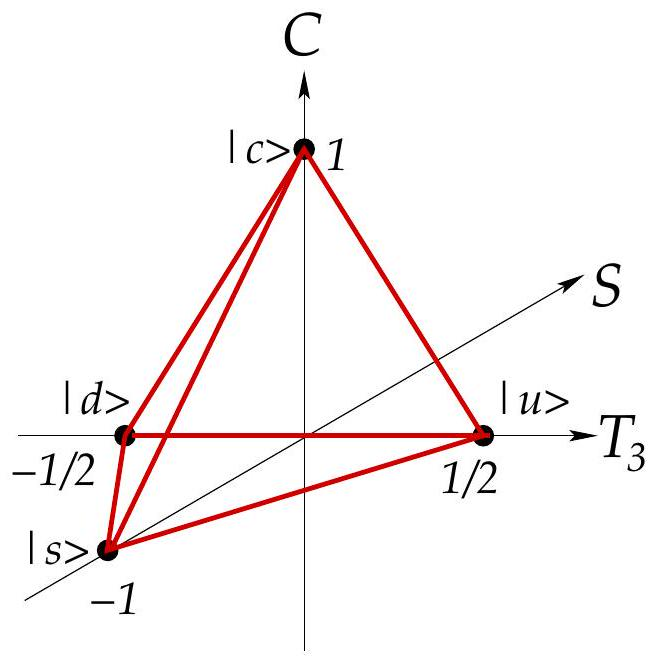
\includegraphics[scale=0.3, center]{2025_05_20_8618f55a41bfe980b4b2g-78}\\
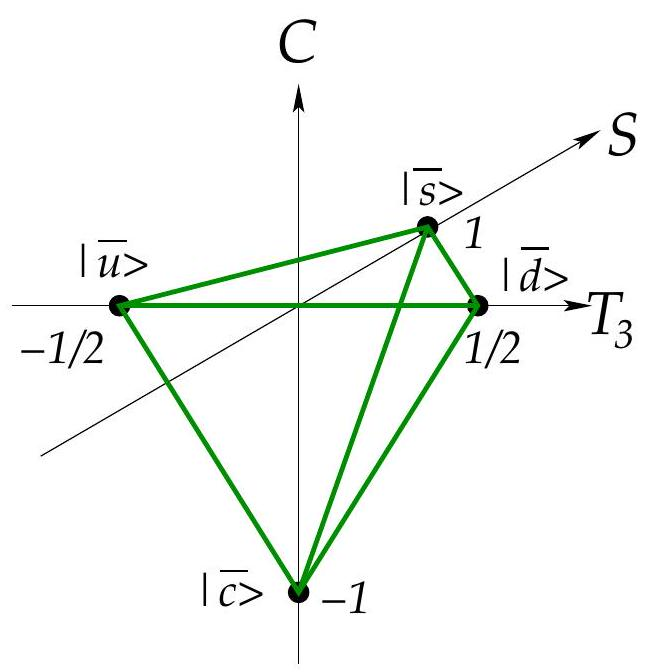
\includegraphics[scale=0.3, center]{2025_05_20_8618f55a41bfe980b4b2g-78(1)}

In the ( $T_{3}-S$ ) plane one observes the ( $S U(3), \cdot$ ) sub-multiplets consisting of up, down, and strange quark (triplet) or of the corresponding anti-quarks (anti-triplet).

Higher multiplets can again be generated by coupling fundamental quadruplets. We list the most important coupling rules (without proof):

$$
\begin{aligned}
{[4] \otimes[\overline{4}] } & =[1] \oplus[15] \\
{[4] \otimes[4] \otimes[4] } & =[\overline{4}] \oplus[20] \oplus[20] \oplus\left[20^{\prime}\right]
\end{aligned}
$$

Accordingly, one finds mesons in ( $S U(4), \cdot$ ) singlets or 15-plets and baryons in ( $S U(4), \cdot$ ) anti-quadruplets as well as three 20 -plets. For the pseudoscalar mesons this is exemplified in the following figure:\\
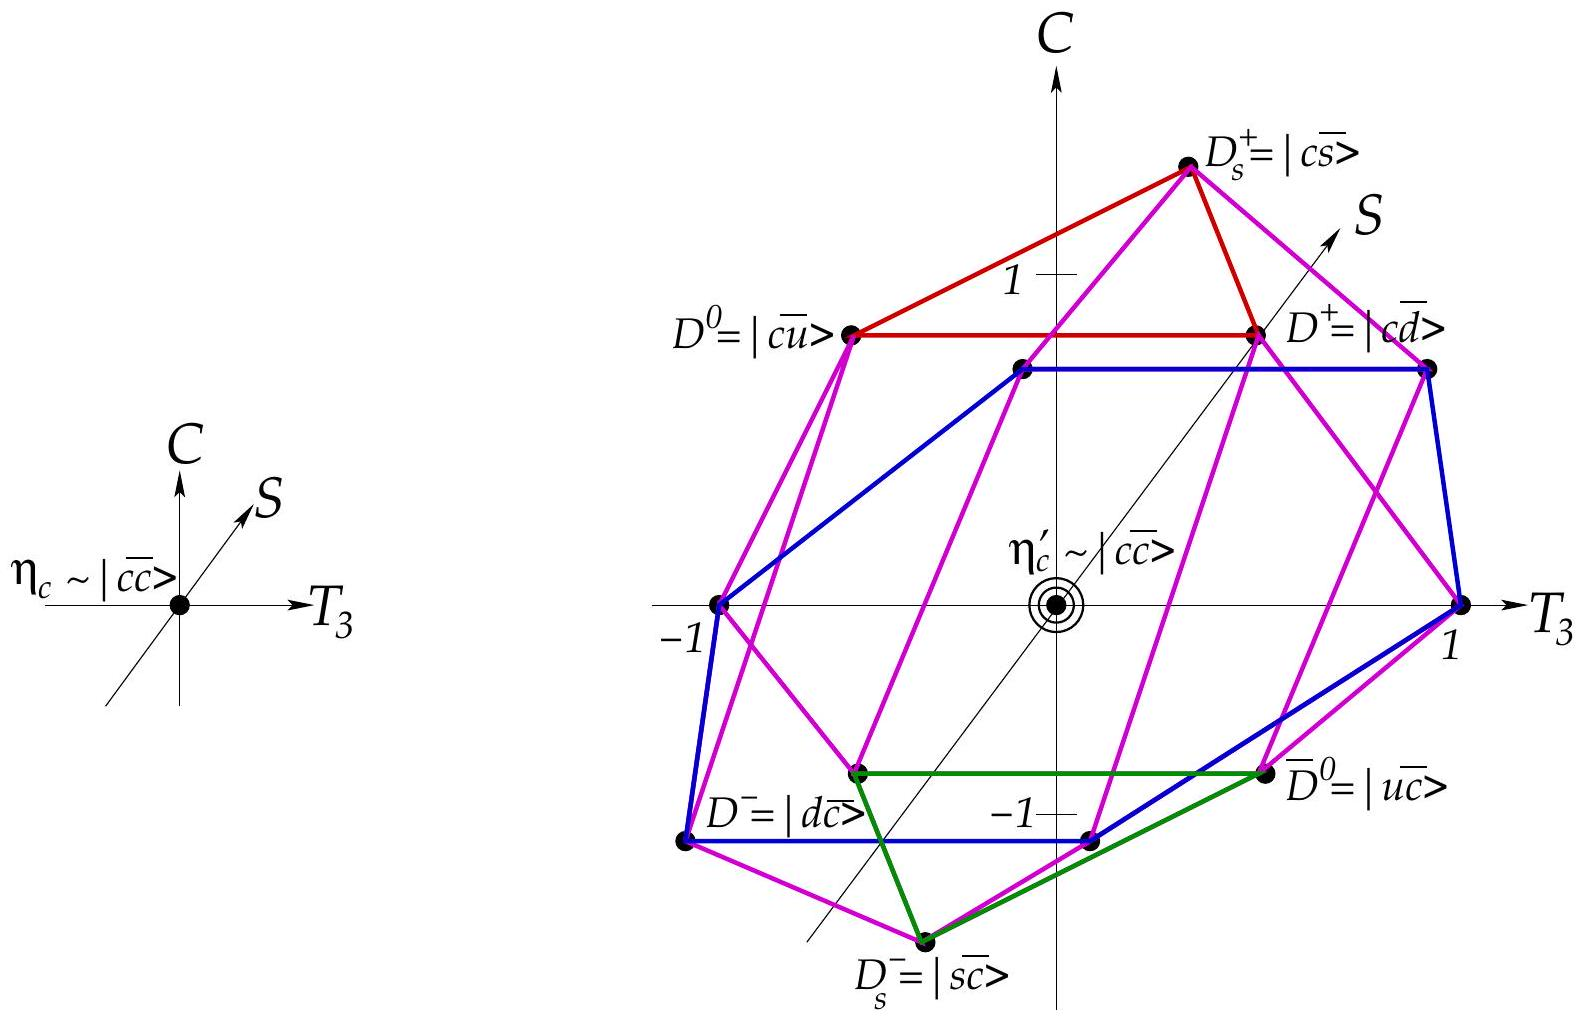
\includegraphics[scale=0.2, center]{2025_05_20_8618f55a41bfe980b4b2g-79}

In the 15 -plet one recognizes one octet (blue) at $C=0$. This is the pseudoscalar-meson octet we have already encountered when discussing the ( $\operatorname{SU}(3), \cdot$ ) flavor symmetry. The individual states are no longer explicitly labelled. New states are an ( $\operatorname{SU}(3), \cdot$ ) triplet (green) at $C=-1$ and an ( $S U(3), \cdot$ ) anti-triplet (red) at $C=1$. The corresponding states are

$$
\begin{aligned}
D^{ \pm}: I\left(J^{P C}\right)=\frac{1}{2}\left(0^{-+}\right), & m_{D^{ \pm}}=1869.5 \pm 0.4 \mathrm{MeV} \\
D^{0}: I\left(J^{P C}\right)=\frac{1}{2}\left(0^{-+}\right), & m_{D^{0}}=1864.91 \pm 0.17 \mathrm{MeV} \\
D_{s}^{ \pm}: I\left(J^{P C}\right)=0\left(0^{-+}\right), & m_{D_{s}^{ \pm}}=1969.0 \pm 1.4 \mathrm{MeV} \\
\eta_{c}: I\left(J^{P C}\right)=0\left(0^{-+}\right), & m_{\eta_{c}}=2981.0 \pm 1.1 \mathrm{MeV} \\
\eta_{c}^{\prime}: I\left(J^{P C}\right)=0\left(0^{-+}\right), & m_{\eta_{c}^{\prime}}=3638.9 \pm 1.3 \mathrm{MeV}
\end{aligned}
$$

The vector meson corresponding to the ( $S U(4), \cdot$ ) singlet $\eta_{c}$, the so-called $J / \Psi$ meson $\left(m_{J / \Psi}=3096.916 \pm 0.011 \mathrm{MeV}\right)$ was the first particle carrying charm which was experimentally detected, in the year 1974 by Samuel Ting at the Alternating Gradient Synchrotron (AGS) of Brookhaven National Laboratory (BNL) on Long Island. For this achievement he received (together with Burton Richter of Stanford Linear Accelerator Center, SLAC) the Nobel prize 1976.

\section{The Poincaré group}
In Chapter 2 we had considered rotations in space. Together with the so-called Lorentz boosts, i.e., transformations between inertial frames encountered in special relativity, they form the so-called Lorentz group $\mathbb{L}$ (or more precisely, the so-called proper orthochronous Lorentz group $\mathbb{L}_{+}^{\uparrow}$, since space-reflection and time-reversal transformations will not be considered). Moreover, we had considered translations in space and time in Chapter 2. Taking these together with the Lorentz group, we obtain the so-called Poincaré group $\mathbb{P}$.

\subsection{Characterization of the Poincaré group}
Let us consider a Poincaré transformation of the space-time position vector,

$$
x^{\mu} \longrightarrow x^{\prime \mu}=\Lambda^{\mu}{ }_{\nu} x^{\nu}+a^{\mu},
$$

i.e., the Lorentz transformation

$$
x^{\mu} \longrightarrow \bar{x}^{\mu}=\Lambda_{\nu}^{\mu} x^{\nu}
$$

of the position vector, followed by a space-time translation by the constant 4 -vector $a^{\mu}$,

$$
\bar{x}^{\mu} \longrightarrow x^{\prime \mu}=\bar{x}^{\mu}+a^{\mu} .
$$

Remark: Of course, one can also first perform the space-time translation,

$$
x^{\mu} \longrightarrow \hat{x}^{\mu}=x^{\mu}+\hat{a}^{\mu},
$$

and then the Lorentz transformation,

$$
\hat{x}^{\mu} \longrightarrow x^{\prime \mu}=\Lambda^{\mu}{ }_{\nu} \hat{x}^{\nu}=\Lambda^{\mu}{ }_{\nu} x^{\mu}+\Lambda^{\mu}{ }_{\nu} \hat{a}^{\nu} .
$$

If we denote $\Lambda^{\mu}{ }_{\nu} \hat{a}^{\nu} \equiv a^{\mu}$, we again obtain Eq. (6.1).\\
Two successive Poincaré transformations can therefore be written as follows:

$$
\begin{aligned}
x^{\mu} \longrightarrow x^{\prime \prime \mu} & =\bar{\Lambda}^{\mu}{ }_{\nu} x^{\prime \nu}+\bar{a}^{\mu} \\
& =\bar{\Lambda}^{\mu}{ }_{\nu}\left(\Lambda^{\nu}{ }_{\rho} x^{\rho}+a^{\nu}\right)+\bar{a}^{\mu} \\
& =\bar{\Lambda}^{\mu}{ }_{\nu} \Lambda^{\nu}{ }_{\rho} x^{\rho}+\bar{\Lambda}^{\mu}{ }_{\nu} a^{\nu}+\bar{a}^{\mu} .
\end{aligned}
$$

Two successive Lorentz transformations yield (because of the closure of the Lorentz group) again a Lorentz transformation, i.e.,

$$
\bar{\Lambda}^{\mu}{ }_{\nu} \Lambda^{\nu}{ }_{\rho} \equiv \hat{\Lambda}^{\mu}{ }_{\rho} \in \mathbb{L} .
$$

If we denote

$$
\hat{a}^{\mu} \equiv \bar{\Lambda}^{\mu}{ }_{\nu} a^{\nu}+\bar{a}^{\mu},
$$

we realize that two successive Poincaré transformations, Eq. 6.6), again yield a Poincaré transformation,

$$
x^{\mu} \longrightarrow x^{\prime \prime \mu}=\hat{\Lambda}_{\rho}^{\mu} x^{\rho}+\hat{a}^{\mu} .
$$

This shows the closure of the Poincaré group. If we consider the transformation of an object in an arbitrary representation of the group instead of the transformation of a 4 -vector $x^{\mu}$, and the corresponding representation of an element of the group, $U(\Lambda, a) \in$ $D(\mathbb{P})$, then Eq. 6.6 reads as follows:

$$
U(\bar{\Lambda}, \bar{a}) U(\Lambda, a)=U(\bar{\Lambda} \Lambda, \bar{\Lambda} a+\bar{a}) \equiv U(\hat{\Lambda}, \hat{a})
$$

The identity element of the Poincaré group has the form $U(1,0)$, so that

$$
U(1,0) U(\Lambda, a)=U(\Lambda, a) U(1,0)=U(\Lambda, a)
$$

The inverse element is

$$
U^{-1}(\Lambda, a) \equiv U\left(\Lambda^{-1},-\Lambda^{-1} a\right) \in D(\mathbb{P})
$$

since according to Eq. 6.10 we have

$$
U^{-1}(\Lambda, a) U(\Lambda, a)=U\left(\Lambda^{-1},-\Lambda^{-1} a\right) U(\Lambda, a)=U\left(\Lambda^{-1} \Lambda, \Lambda^{-1} a-\Lambda^{-1} a\right) \equiv U(1,0)
$$

With Eq. 6.10 we compute on the one hand

$$
U(\hat{\Lambda}, \hat{a}) U(\bar{\Lambda}, \bar{a}) U(\Lambda, a)=U(\hat{\Lambda}, \hat{a}) U(\bar{\Lambda} \Lambda, \bar{\Lambda} a+\bar{a})=U(\hat{\Lambda} \bar{\Lambda} \Lambda, \hat{\Lambda} \bar{\Lambda} a+\hat{\Lambda} \bar{a}+\hat{a})
$$

and on the other hand

$$
U(\hat{\Lambda}, \hat{a}) U(\bar{\Lambda}, \bar{a}) U(\Lambda, a)=U(\hat{\Lambda} \bar{\Lambda}, \hat{\Lambda} \bar{a}+\hat{a}) U(\Lambda, a)=U(\hat{\Lambda} \bar{\Lambda} \Lambda, \hat{\Lambda} \bar{\Lambda} a+\hat{\Lambda} \bar{a}+\hat{a})
$$

Comparison of Eq. (6.14) with 6.15 proves the law of associativity for the Poincaré group. With Eqs. 6.10, 6.11, 6.12, 6.14, and 6.15 we have proven that the Poincaré group fulfills the group axioms.

\subsection{Generators}
The Poincaré group is a Lie group, i.e., each element $U(\Lambda, a)$ has a representation as a linear operator,

$$
\hat{U}(\vec{\alpha})=\exp \left(-i \sum_{j=1}^{N} \alpha_{j} \hat{X}_{j}\right)
$$

cf. Eq. (3.10) (using natural units $\hbar=c=1$ ). How many generators (or parameters, respectively) are there? Four generators enact translations in the three spatial directions\\
and in time. We know them already from the discussion in Chapter 2; they can be compactly written as a 4 -vector:

$$
\hat{P}^{\mu}=i \partial^{\mu}=i\left(\frac{\partial}{\partial t},-\vec{\nabla}\right)^{T},
$$

where the right-hand side of the equation corresponds to the representation of $\hat{P}^{\mu}$ as linear differential operator. On the other hand, the Lorentz group has six generators, three for rotations around the three spatial axes and three for boosts in each spatial direction. Thus, the Poincaré group has ten generators.

The four generators (6.17) of space-time translations we have already encountered. But what are the six generators of the Lorentz group? We first write these generators compactly in the form of an antisymmetric Lorentz tensor of rank $2, \hat{J}^{\mu \nu}=-\hat{J}^{\nu \mu}$. The relationship to the generators of rotations (which of course have to correspond to the angular momentum operator) and to that of the boosts will be discussed later. One readily convinces oneself of the fact that due to the antisymmetry of $\hat{J}^{\mu \nu}$, only six of the 16 possible components are independent. Then we can write Eq. (6.16) in the form

$$
\hat{U}(\omega, a)=\exp \left(-\frac{i}{2} \omega_{\mu \nu} \hat{J}^{\mu \nu}+i a_{\mu} \hat{P}^{\mu}\right) .
$$

The four parameters of space-time translations are summarized in the constant 4 -vector $a^{\mu}$. The choice of sign in front of the translation part corresponds to the convention used in Chapter 2. The six parameters of Lorentz transformations we have written as components of a rank- 2 tensor $\omega^{\mu \nu}$. This tensor can also be chosen to be antisymmetric, $\omega^{\mu \nu}=$ $-\omega^{\nu \mu}$, since any possibly existing symmetric part would vanish anyway after complete contraction with the antisymmetric tensor $\hat{J}^{\mu \nu}$, thus does not need to be considered. The six parameters are on the one hand the three angles for rotations around the $x, y$, and $z$ directions, and on the other hand the three rapidities for boosts along these spatial directions.

In order to see this, let us look at the explicit form of the Lorentz-transformation matrix. A spatial rotation, e.g. around the angle $\phi$ around the $z$ axis, is enacted by

$$
\Lambda_{D \beta}^{\alpha}(0,0, \phi)=\left(\begin{array}{cccc}
1 & 0 & 0 & 0 \\
0 & \cos \phi & \sin \phi & 0 \\
0 & -\sin \phi & \cos \phi & 0 \\
0 & 0 & 0 & 1
\end{array}\right),
$$

For an infinitesimal angle $\phi \ll 1$ this reads

$$
\Lambda_{D \beta}^{\alpha}(0,0, \phi)=\left(\begin{array}{cccc}
1 & 0 & 0 & 0 \\
0 & 1 & \phi & 0 \\
0 & -\phi & 1 & 0 \\
0 & 0 & 0 & 1
\end{array}\right) \equiv g^{\alpha}{ }_{\beta}+\phi\left(g^{\alpha 2} g^{1}{ }_{\beta}-g^{\alpha 1} g^{2}{ }_{\beta}\right) .
$$

A boost, e.g. with rapidity $\chi$ in $z$ direction, is enacted by

$$
\Lambda_{B \beta}^{\alpha}(0,0, \chi)=\left(\begin{array}{cccc}
\cosh \chi & 0 & 0 & -\sinh \chi \\
0 & 1 & 0 & 0 \\
0 & 0 & 1 & 0 \\
-\sinh \chi & 0 & 0 & \cosh \chi
\end{array}\right) .
$$

For infinitesimal rapidities $\chi \ll 1$ this reads

$$
\Lambda_{B \beta}^{\alpha}(0,0, \chi)=\left(\begin{array}{cccc}
1 & 0 & 0 & -\chi \\
0 & 1 & 0 & 0 \\
0 & 0 & 1 & 0 \\
-\chi & 0 & 0 & 1
\end{array}\right)=g_{\beta}^{\alpha}+\chi\left(g^{\alpha 3} g_{\beta}^{0}-g^{\alpha 0} g_{\beta}^{3}\right)
$$

For arbitrary infinitesimal Lorentz transformations, Eqs. (6.20) and (6.22) can be generalized as

$$
\Lambda_{\beta}^{\alpha}=g_{\beta}^{\alpha}+\omega_{\beta}^{\alpha},
$$

with the antisymmetric tensor $\omega^{\alpha}{ }_{\beta}$ of the parameters of Lorentz transformations.\\
Let us remark that the representation (6.18) of an element of the Poincaré group as linear operator is not yet completely determined. It depends on which irreducible representation of the group this linear operator is supposed to act. This then influences the form of the generators.

\subsection{The Poincaré algebra}
We now determine the Poincaré algebra fulfilled by the generators $\hat{J}^{\mu \nu}$ and $\hat{P}^{\mu}$. To this end we first consider how the generators behave under Poincaré transformations. An arbitrary infinitesimal Poincaré transformation can be written as $U(1+\omega, \epsilon)$, where on account of Eq. 6.23) we have written an infinitesimal Lorentz transformation compactly as $\Lambda \equiv 1+\omega$, with the tensor $\omega^{\mu \nu}$ of the infinitesimal parameters of rotations and boosts, and we have introduced an infinitesimal space-time translation vector $\epsilon^{\mu}$. We now compute using Eq. 6.10

$$
\begin{aligned}
U(\Lambda, a) U(1+\omega, \epsilon) U^{-1}(\Lambda, a) & =U(\Lambda(1+\omega), \Lambda \epsilon+a) U\left(\Lambda^{-1},-\Lambda^{-1} a\right) \\
& =U\left(\Lambda(1+\omega) \Lambda^{-1},-\Lambda(1+\omega) \Lambda^{-1} a+\Lambda \epsilon+a\right) \\
& =U\left(1+\Lambda \omega \Lambda^{-1}, \Lambda \epsilon-\Lambda \omega \Lambda^{-1} a\right)
\end{aligned}
$$

Using Eq. 6.18 and expanding the left-hand and right-hand sides to leading order in the infinitesimal parameters,

$$
\begin{aligned}
& U(\Lambda, a)\left(1-\frac{i}{2} \omega_{\mu \nu} \hat{J}^{\mu \nu}+i \epsilon_{\mu} \hat{P}^{\mu}\right) U^{-1}(\Lambda, a) \\
& \quad=1-\frac{i}{2} \omega_{\mu \nu} U(\Lambda, a) \hat{J}^{\mu \nu} U^{-1}(\Lambda, a)+i \epsilon_{\mu} U(\Lambda, a) \hat{P}^{\mu} U^{-1}(\Lambda, a) \\
& \quad=1-\frac{i}{2} \Lambda_{\mu \rho} \omega^{\rho}{ }_{\sigma}\left(\Lambda^{-1}\right)^{\sigma}{ }_{\nu} \hat{J}^{\mu \nu}+i\left(\Lambda_{\mu \rho} \epsilon^{\rho}-\Lambda_{\mu \rho} \omega^{\rho}{ }_{\sigma}\left(\Lambda^{-1}\right)^{\sigma}{ }_{\nu} a^{\nu}\right) \hat{P}^{\mu} \\
& \quad=1-\frac{i}{2}\left(\Lambda_{\mu \rho} \omega^{\rho}{ }_{\sigma} \Lambda_{\nu}{ }^{\sigma} \hat{J}^{\mu \nu}+\Lambda_{\mu \rho} \omega^{\rho}{ }_{\sigma} \Lambda_{\nu}{ }^{\sigma} a^{\nu} \hat{P}^{\mu}-\Lambda_{\mu \rho} \omega_{\sigma}{ }^{\rho} \Lambda_{\nu}{ }^{\sigma} a^{\nu} \hat{P}^{\mu}\right)+i \Lambda_{\mu \rho} \epsilon^{\rho} \hat{P}^{\mu}
\end{aligned}
$$

where we have employed the property $\Lambda^{-1}=g^{-1} \Lambda^{T} g$ of the Lorentz-transformation matrices and the antisymmetry of $\omega^{\mu \nu}$. We now relabel the indices $\mu \leftrightarrow \nu$ and $\rho \leftrightarrow \sigma$ in the\\
last term in parentheses and obtain after subtracting one and multiplying both sides with $2 i$

$$
U(\Lambda, a)\left(\omega_{\mu \nu} \hat{J}^{\mu \nu}-2 \epsilon_{\mu} \hat{P}^{\mu}\right) U^{-1}(\Lambda, a)=\Lambda_{\mu \rho} \omega_{\sigma}^{\rho} \Lambda_{\nu}^{\sigma}\left(\hat{J}^{\mu \nu}+a^{\nu} \hat{P}^{\mu}-a^{\mu} \hat{P}^{\nu}\right)-2 \Lambda_{\mu \rho} \epsilon^{\rho} \hat{P}^{\mu}
$$

A further relabelling of indices on the right-hand side ( $\mu \leftrightarrow \rho, \nu \leftrightarrow \sigma$ ) leads to

$$
U(\Lambda, a)\left(\omega_{\mu \nu} \hat{J}^{\mu \nu}-2 \epsilon_{\mu} \hat{P}^{\mu}\right) U^{-1}(\Lambda, a)=\Lambda_{\rho \mu} \omega_{\nu}^{\mu} \Lambda_{\sigma}^{\nu}\left(\hat{J}^{\rho \sigma}+a^{\sigma} \hat{P}^{\rho}-a^{\rho} \hat{P}^{\sigma}\right)-2 \Lambda_{\rho \mu} \epsilon^{\mu} \hat{P}^{\rho}
$$

The parameters $\omega_{\mu \nu}$ and $\epsilon_{\mu}$ can be chosen arbitrarily, so that one can compare their coefficients on the left- and right-hand side to obtain the transformation behavior of the generators:

$$
\begin{aligned}
U(\Lambda, a) \hat{J}^{\mu \nu} U^{-1}(\Lambda, a) & =\Lambda_{\rho}{ }^{\mu} \Lambda_{\sigma}{ }^{\nu}\left(\hat{J}^{\rho \sigma}+a^{\sigma} \hat{P}^{\rho}-a^{\rho} \hat{P}^{\sigma}\right) \\
U(\Lambda, a) \hat{P}^{\mu} U^{-1}(\Lambda, a) & =\Lambda_{\rho}{ }^{\mu} \hat{P}^{\rho}
\end{aligned}
$$

We now consider the infinitesimal form of Eqs. 6.28) and (6.29), i.e., for $\Lambda \equiv 1+\omega$ and $a \equiv \epsilon$. To first order in infinitesimal parameters we obtain from Eq. 6.28)

$$
\begin{aligned}
& \left(1-\frac{i}{2} \omega_{\rho \sigma} \hat{J}^{\rho \sigma}+i \epsilon_{\rho} \hat{P}^{\rho}\right) \hat{J}^{\mu \nu}\left(1+\frac{i}{2} \omega_{\alpha \beta} \hat{J}^{\alpha \beta}-i \epsilon_{\alpha} \hat{P}^{\alpha}\right) \\
& =\hat{J}^{\mu \nu}-\frac{i}{2} \omega_{\rho \sigma}\left[\hat{J}^{\rho \sigma}, \hat{J}^{\mu \nu}\right]+i \epsilon_{\rho}\left[\hat{P}^{\rho}, \hat{J}^{\mu \nu}\right] \\
& =\left(g_{\rho}{ }^{\mu}+\omega_{\rho}{ }^{\mu}\right)\left(g_{\sigma}{ }^{\nu}+\omega_{\sigma}{ }^{\nu}\right)\left(\hat{J}^{\rho \sigma}+\epsilon^{\sigma} \hat{P}^{\rho}-\epsilon^{\rho} \hat{P}^{\sigma}\right) \\
& =\hat{J}^{\mu \nu}+\epsilon^{\nu} \hat{P}^{\mu}-\epsilon^{\mu} \hat{P}^{\nu}+\omega_{\rho}{ }^{\mu} \hat{J}^{\rho \nu}+\omega_{\sigma}{ }^{\nu} \hat{J}^{\mu \sigma} \\
& =\hat{J}^{\mu \nu}+\epsilon_{\rho}\left(g^{\rho \nu} \hat{P}^{\mu}-g^{\rho \mu} \hat{P}^{\nu}\right)+\omega_{\rho \sigma}\left(g^{\sigma \mu} \hat{J}^{\rho \nu}-g^{\rho \nu} \hat{J}^{\mu \sigma}\right) \\
& =\hat{J}^{\mu \nu}+\epsilon_{\rho}\left(g^{\rho \nu} \hat{P}^{\mu}-g^{\rho \mu} \hat{P}^{\nu}\right)+\frac{1}{2} \omega_{\rho \sigma}\left(g^{\sigma \mu} \hat{J}^{\rho \nu}-g^{\rho \mu} \hat{J}^{\sigma \nu}-g^{\rho \nu} \hat{J}^{\mu \sigma}+g^{\sigma \nu} \hat{J}^{\mu \rho}\right)
\end{aligned}
$$

where in the last step we have doubled the last term, accounting for that by an additional factor of $1 / 2$, relabelled the indices $\rho \leftrightarrow \sigma$, and finally used the antisymmetry of $\omega_{\rho \sigma}$. Comparing the coefficients of $\omega_{\rho \sigma}$ and $\epsilon_{\rho}$ in the second and sixth line, we obtain the commutation relations

$$
\begin{aligned}
{\left[\hat{J}^{\rho \sigma}, \hat{J}^{\mu \nu}\right] } & =i\left(g^{\sigma \mu} \hat{J}^{\rho \nu}-g^{\rho \mu} \hat{J}^{\sigma \nu}-g^{\rho \nu} \hat{J}^{\mu \sigma}+g^{\sigma \nu} \hat{J}^{\mu \rho}\right) \\
{\left[\hat{P}^{\rho}, \hat{J}^{\mu \nu}\right] } & =i\left(g^{\rho \mu} \hat{P}^{\nu}-g^{\rho \nu} \hat{P}^{\mu}\right)
\end{aligned}
$$

We perform a completely analogous calculation for Eq. 6.29):

$$
\begin{aligned}
& \left(1-\frac{i}{2} \omega_{\rho \sigma} \hat{J}^{\rho \sigma}+i \epsilon_{\rho} \hat{P}^{\rho}\right) \hat{P}^{\mu}\left(1+\frac{i}{2} \omega_{\alpha \beta} \hat{J}^{\alpha \beta}-i \epsilon_{\alpha} \hat{P}^{\alpha}\right) \\
& =\hat{P}^{\mu}-\frac{i}{2} \omega_{\rho \sigma}\left[\hat{J}^{\rho \sigma}, \hat{P}^{\mu}\right]+i \epsilon_{\rho}\left[\hat{P}^{\rho}, \hat{P}^{\mu}\right] \\
& =\left(g_{\rho}{ }^{\mu}+\omega_{\rho}{ }^{\mu}\right) \hat{P}^{\rho} \\
& =\hat{P}^{\mu}+\frac{1}{2} \omega_{\rho \sigma}\left(g^{\sigma \mu} \hat{P}^{\rho}-g^{\rho \mu} \hat{P}^{\sigma}\right)
\end{aligned}
$$

Comparison of coefficients in the second and fourth line leads on the hand again to Eq. 6.32) (after a suitable relabelling of indices), and on the other hand to

$$
\left[\hat{P}^{\rho}, \hat{P}^{\mu}\right]=0
$$

Equations (6.31), 6.32), and (6.34) represent the Poincaré algebra. From Eqs. (6.32) and 6.34) follows that there is an (abelian) ideal, thus the Poincare group is not a (semi-)simple group. Since the group of space-time translations is not compact, the Poincaré is also not a compact group.

If we identify

$$
\begin{aligned}
\hat{P}^{0} & \equiv \hat{H} \\
\hat{\vec{J}} & \equiv\left(\hat{J}^{23}, \hat{J}^{31}, \hat{J}^{12}\right)^{T} \\
\hat{\vec{K}} & \equiv\left(\hat{J}^{01}, \hat{J}^{02}, \hat{J}^{03}\right)^{T}
\end{aligned}
$$

where $\hat{\vec{J}}$ is the operator of total angular momentum (i.e., the sum of orbital angular momentum and spin) and $\hat{\vec{K}}$ is the boost operator, the Poincaré algebra 6.31, 6.32), and 6.34 can be brought into the following form:

$$
\begin{aligned}
{\left[\hat{J}^{i}, \hat{J}^{j}\right] } & =i \epsilon^{i j k} \hat{J}^{k}, \quad\left[\hat{J}^{i}, \hat{K}^{j}\right]=i \epsilon^{i j k} \hat{K}^{k} \\
{\left[\hat{K}^{i}, \hat{K}^{j}\right] } & =-i \epsilon^{i j k} \hat{J}^{k}, \quad\left[\hat{J}^{i}, \hat{P}^{j}\right]=i \epsilon^{i j k} \hat{P}^{k} \\
{\left[\hat{K}^{i}, \hat{P}^{j}\right] } & =-i \hat{H} \delta^{i j} \quad\left[\hat{K}^{i}, \hat{H}\right]=-i \hat{P}^{i} \\
{\left[\hat{J}^{i}, \hat{H}\right] } & =\left[\hat{P}^{i}, \hat{H}\right]=0
\end{aligned}
$$

We leave the proof as homework exercise. The first commutation relation is, of course, obvious, since it represents the angular-momentum algebra. This holds for orbital angular momentum as well as for spin, and thus also for total angular momentum.

\subsubsection{5}
\subsection{Casimir operators}
We define the so-called Pauli-Lubanski pseudovector

$$
\hat{W}_{\mu} \equiv \frac{1}{2} \epsilon_{\mu \nu \rho \sigma} \hat{J}^{\nu \rho} \hat{P}^{\sigma}
$$

Here, $\epsilon_{\mu \nu \rho \sigma}$ is the completely antisymmetric tensor of rank 4 , with $\epsilon^{0123}=+1$. It fulfills the contraction formula

$$
\epsilon^{\mu \nu \alpha \beta} \epsilon_{\mu \tau \rho \sigma}=g_{\tau}^{\nu}\left(g_{\sigma}^{\alpha} g_{\rho}^{\beta}-g_{\rho}^{\alpha} g_{\sigma}^{\beta}\right)+g_{\rho}^{\nu}\left(g_{\tau}^{\alpha} g_{\sigma}^{\beta}-g_{\sigma}^{\alpha} g_{\tau}^{\beta}\right)+g_{\sigma}^{\nu}\left(g_{\rho}^{\alpha} g_{\tau}^{\beta}-g_{\tau}^{\alpha} g_{\rho}^{\beta}\right)
$$

A further contraction over the second index yields

$$
\begin{aligned}
\epsilon^{\mu \nu \alpha \beta} \epsilon_{\mu \nu \rho \sigma} & =4\left(g_{\sigma}^{\alpha} g_{\rho}^{\beta}-g_{\rho}^{\alpha} g_{\sigma}^{\beta}\right)+g_{\rho}^{\alpha} g_{\sigma}^{\beta}-g_{\sigma}^{\alpha} g_{\rho}^{\beta}+g_{\rho}^{\alpha} g_{\sigma}^{\beta}-g_{\sigma}^{\alpha} g_{\rho}^{\beta} \\
& =2\left(g_{\sigma}^{\alpha} g_{\rho}^{\beta}-g_{\rho}^{\alpha} g_{\sigma}^{\beta}\right) .
\end{aligned}
$$

The Pauli-Lubanski pseudovector is orthogonal to the 4 -momentum vector. Namely, using Eq. (6.34), we obtain

$$
\begin{aligned}
\hat{W}_{\mu} \hat{P}^{\mu} & =\frac{1}{2} \epsilon_{\mu \nu \rho \sigma} \hat{J}^{\nu \rho} \hat{P}^{\sigma} \hat{P}^{\mu}=\frac{1}{2} \epsilon_{\mu \nu \rho \sigma} \hat{J}^{\nu \rho} \hat{P}^{\mu} \hat{P}^{\sigma}=\frac{1}{2} \epsilon_{\sigma \nu \rho \mu} \hat{J}^{\nu \rho} \hat{P}^{\sigma} \hat{P}^{\mu} \\
& =-\frac{1}{2} \epsilon_{\mu \nu \rho \sigma} \hat{J}^{\nu \rho} \hat{P}^{\sigma} \hat{P}^{\mu}=-\hat{W}_{\mu} \hat{P}^{\mu} \equiv 0
\end{aligned}
$$

where in the last step of the first line we relabelled indices $\sigma \leftrightarrow \mu$ and to the second line we have used the antisymmetry of the tensor $\epsilon_{\mu \nu \rho \sigma}$.\\
Proposition: The following two operators are the two Casimir operators of the Poincaré group:

$$
\hat{P}^{2}=\hat{P}_{\mu} \hat{P}^{\mu} \quad \text { und } \quad \hat{W}^{2}=\hat{W}_{\mu} \hat{W}^{\mu}
$$

Remark: According to Eqs. (6.31), (6.32), and (6.34) the Poincaré algebra contains an abelian ideal, consisting of the generators of space-time translations. Thus, it is not a semi-simple group, therefore Racah's theorem does not apply to draw a conclusion about the number of generators from the rank of the group. However, it is in fact true that the two operators given in Eq. 6.43) are the only Casimir operators of the Poincaré group.\\
Proof: We first show that $\hat{P}^{2}$ commutes with all generators of the group. Using the Poincaré algebra (6.31), 6.32), and 6.34 we obtain

$$
\begin{aligned}
{\left[\hat{P}^{2}, \hat{P}^{\rho}\right] } & =g_{\mu \nu}\left[\hat{P}^{\mu} \hat{P}^{\nu}, \hat{P}^{\rho}\right]=g_{\mu \nu}\left\{\hat{P}^{\mu}\left[\hat{P}^{\nu}, \hat{P}^{\rho}\right]+\left[\hat{P}^{\mu}, \hat{P}^{\rho}\right] \hat{P}^{\nu}\right\}=0 \\
{\left[\hat{P}^{2}, \hat{J}^{\rho \sigma}\right] } & =g_{\mu \nu}\left[\hat{P}^{\mu} \hat{P}^{\nu}, \hat{J}^{\rho \sigma}\right]=g_{\mu \nu}\left\{\hat{P}^{\mu}\left[\hat{P}^{\nu}, \hat{J}^{\rho \sigma}\right]+\left[\hat{P}^{\mu}, \hat{J}^{\rho \sigma}\right] \hat{P}^{\nu}\right\} \\
& =i g_{\mu \nu}\left\{\hat{P}^{\mu}\left(g^{\nu \rho} \hat{P}^{\sigma}-g^{\nu \sigma} \hat{P}^{\rho}\right)+\left(g^{\mu \rho} \hat{P}^{\sigma}-g^{\mu \sigma} \hat{P}^{\rho}\right) \hat{P}^{\nu}\right\} \\
& =i\left(\hat{P}^{\rho} \hat{P}^{\sigma}-\hat{P}^{\sigma} \hat{P}^{\rho}+\hat{P}^{\sigma} \hat{P}^{\rho}-\hat{P}^{\rho} \hat{P}^{\sigma}\right)=0
\end{aligned}
$$

Now we show that $\hat{W}^{2}$ commutes with all generators of the group. First, on account of the commutation relations $(\boxed{6.32})$ and $(6.34)$ we conclude that

$$
\begin{aligned}
{\left[\hat{W}^{\alpha}, \hat{P}^{\mu}\right] } & =\frac{1}{2} \epsilon^{\alpha}{ }_{\nu \rho \sigma}\left[\hat{J}^{\nu \rho} \hat{P}^{\sigma}, \hat{P}^{\mu}\right] \\
& =\frac{1}{2} \epsilon^{\alpha}{ }_{\nu \rho \sigma}\left\{\hat{J}^{\nu \rho}\left[\hat{P}^{\sigma}, \hat{P}^{\mu}\right]+\left[\hat{J}^{\nu \rho}, \hat{P}^{\mu}\right] \hat{P}^{\sigma}\right\} \\
& =-\frac{i}{2} \epsilon^{\alpha}{ }_{\nu \rho \sigma}\left(g^{\mu \nu} \hat{P}^{\rho}-g^{\mu \rho} \hat{P}^{\nu}\right) \hat{P}^{\sigma} \\
& =-\frac{i}{2}\left(\epsilon^{\alpha \mu \nu \sigma}-\epsilon^{\alpha \nu \mu \sigma}\right) \hat{P}_{\nu} \hat{P}_{\sigma}=-\frac{i}{2} \epsilon^{\alpha \mu \nu \sigma}\left[\hat{P}_{\nu}, \hat{P}_{\sigma}\right] \equiv 0
\end{aligned}
$$

where to the last line we have relabelled the indices $\rho \leftrightarrow \nu$ in the first term and then in the next-to-last step used the antisymmetry of $\epsilon^{\mu \alpha \nu \sigma}$.

Furthermore, we require

$$
\left[\hat{W}^{\alpha}, \hat{J}^{\mu \nu}\right]=i\left(g^{\alpha \mu} \hat{W}^{\nu}-g^{\alpha \nu} \hat{W}^{\mu}\right)
$$

The proof of this relation utilizes the definition of a new tensor,

$$
\tilde{J}_{\mu \nu} \equiv \frac{1}{2} \epsilon_{\mu \nu \rho \sigma} \hat{J}^{\rho \sigma}
$$

Contracting from the left with $\epsilon^{\alpha \beta \mu \nu}$ and multiplying by $-1 / 2$ we obtain using Eq. 6.41) and the antisymmetry of $\hat{J}^{\rho \sigma}$

$$
-\frac{1}{2} \epsilon^{\alpha \beta \mu \nu} \tilde{J}_{\mu \nu}=-\frac{1}{4} \epsilon^{\alpha \beta \mu \nu} \epsilon_{\mu \nu \rho \sigma} \hat{J}^{\rho \sigma}=\frac{1}{2}\left(g^{\alpha}{ }_{\rho} g^{\beta}{ }_{\sigma}-g^{\alpha}{ }_{\sigma} g^{\beta}{ }_{\rho}\right) \hat{J}^{\rho \sigma} \equiv \hat{J}^{\alpha \beta} .
$$

In order to prove Eq. (6.46), we need the following commutation relation:

$$
\begin{aligned}
{\left[\tilde{J}^{\rho \sigma}, \hat{J}^{\mu \nu}\right] } & =\frac{1}{2} \epsilon^{\rho \sigma}{ }_{\alpha \beta}\left[\hat{J}^{\alpha \beta}, \hat{J}^{\mu \nu}\right] \\
& =\frac{i}{2} \epsilon^{\rho \sigma}{ }_{\alpha \beta}\left(g^{\beta \mu} \hat{J}^{\alpha \nu}-g^{\alpha \mu} \hat{J}^{\beta \nu}-g^{\alpha \nu} \hat{J}^{\mu \beta}+g^{\beta \nu} \hat{J}^{\mu \alpha}\right) \\
& =\frac{i}{2}\left(\epsilon^{\rho \sigma \alpha \mu} \hat{J}_{\alpha}{ }^{\nu}-\epsilon^{\rho \sigma \mu \beta} \hat{J}_{\beta}{ }^{\nu}-\epsilon^{\rho \sigma \nu \beta} \hat{J}^{\mu}{ }_{\beta}+\epsilon^{\rho \sigma \alpha \nu} \hat{J}^{\mu}{ }_{\alpha}\right) \\
& =-i\left(\epsilon^{\rho \sigma \mu \alpha} \hat{J}_{\alpha}{ }^{\nu}-\epsilon^{\rho \sigma \nu \alpha} \hat{J}_{\alpha}{ }^{\mu}\right)
\end{aligned}
$$

Here we have used Eq. (6.31) for the second step and relabelled the indices in the second and third term $(\beta \rightarrow \alpha)$ for the fourth step. Furthermore, we exploited the antisymmetry of $\epsilon_{\alpha \beta \mu \rho}$ and $\hat{J}^{\mu \nu}$. Inserting Eq. 6.48, we obtain using Eq. 6.40

$$
\begin{aligned}
& {\left[\begin{array}{ll}
\tilde{J}^{\rho \sigma}, & \hat{J}^{\mu \nu}
\end{array}\right]=\frac{i}{2}\left(\epsilon^{\rho \sigma \mu \alpha} \epsilon_{\alpha}^{\nu \beta \gamma}-\epsilon^{\rho \sigma \nu \alpha} \epsilon_{\alpha}^{\mu \beta \gamma}\right) \tilde{J}_{\beta \gamma}} \\
& =-\frac{i}{2}\left[g^{\mu \nu}\left(g^{\rho \gamma} g^{\sigma \beta}-g^{\rho \beta} g^{\sigma \gamma}\right)+g^{\mu \beta}\left(g^{\rho \nu} g^{\sigma \gamma}-g^{\rho \gamma} g^{\sigma \nu}\right)+g^{\mu \gamma}\left(g^{\rho \beta} g^{\sigma \nu}-g^{\rho \nu} g^{\sigma \beta}\right)\right. \\
& \quad \quad-(\mu \leftrightarrow \nu)] \tilde{J}_{\beta \gamma} \\
& =-i\left(g^{\rho \nu} \tilde{J}^{\mu \sigma}-g^{\rho \mu} \tilde{J}^{\nu \sigma}-g^{\sigma \nu} \tilde{J}^{\mu \rho}+g^{\sigma \mu} \tilde{J}^{\nu \rho}\right) \\
& =i\left(g^{\sigma \mu} \tilde{J}^{\rho \nu}-g^{\rho \mu} \tilde{J}^{\sigma \nu}-g^{\rho \nu} \tilde{J}^{\mu \sigma}+g^{\sigma \nu} \tilde{J}^{\mu \rho}\right)
\end{aligned}
$$

where to the next-to-last step we have used the an antisymmetry of $\tilde{J}^{\mu \nu}$ and to the last step reordererd the terms somewhat (again using the antisymmetry of $\tilde{J}^{\mu \nu}$ ). Comparison with Eq. 6.31, reveals that $\tilde{J}^{\rho \sigma}$ fulfulls the same commutation relation with $\hat{J}^{\mu \nu}$ as $\hat{J}^{\rho \sigma}$ with itself.

An important property of the tensor $\tilde{J}^{\mu \nu}$ is

$$
\begin{aligned}
\hat{P}^{\nu} \tilde{J}_{\mu \nu} & =\frac{1}{2} \epsilon_{\mu \nu \rho \sigma} \hat{P}^{\nu} \hat{J}^{\rho \sigma}=\frac{1}{2} \epsilon_{\mu \rho \sigma \nu} \hat{P}^{\nu} \hat{J}^{\rho \sigma} \\
& =\frac{1}{2} \epsilon_{\mu \rho \sigma \nu}\left\{\hat{J}^{\rho \sigma} \hat{P}^{\nu}+\left[\hat{P}^{\nu}, \hat{J}^{\rho \sigma}\right]\right\} \\
& =\hat{W}_{\mu}+\frac{i}{2} \epsilon_{\mu \rho \sigma \nu}\left(g^{\nu \rho} \hat{P}^{\sigma}-g^{\nu \sigma} \hat{P}^{\rho}\right) \equiv \hat{W}_{\mu}
\end{aligned}
$$

Here we have made use of the definition (6.39) of the Pauli-Lubanski pseudovector, of the commutation relation 6.32, as well as of the antisymmetry of $\epsilon_{\mu \rho \sigma \nu}$.

Using the relations (6.50) and (6.51), as well as Eq. (6.32), we prove Eq. 6.46):

$$
\begin{aligned}
{\left[\hat{W}^{\alpha}, \hat{J}^{\mu \nu}\right] } & =\left[\hat{P}_{\beta} \tilde{J}^{\alpha \beta}, \hat{J}^{\mu \nu}\right]=\hat{P}_{\beta}\left[\tilde{J}^{\alpha \beta}, \hat{J}^{\mu \nu}\right]+g_{\beta \rho}\left[\hat{P}^{\rho}, \hat{J}^{\mu \nu}\right] \tilde{J}^{\alpha \beta} \\
& =i \hat{P}_{\beta}\left(g^{\beta \mu} \tilde{J}^{\alpha \nu}-g^{\alpha \mu} \tilde{J}^{\beta \nu}-g^{\alpha \nu} \tilde{J}^{\mu \beta}+g^{\beta \nu} \tilde{J}^{\mu \alpha}\right)+i g_{\beta \rho}\left(g^{\rho \mu} \hat{P}^{\nu}-g^{\rho \nu} \hat{P}^{\mu}\right) \tilde{J}^{\alpha \beta} \\
& =i\left(\hat{P}^{\mu} \tilde{J}^{\alpha \nu}+g^{\alpha \mu} \hat{W}^{\nu}-g^{\alpha \nu} \hat{W}^{\mu}+\hat{P}^{\nu} \tilde{J}^{\mu \alpha}+\hat{P}^{\nu} \tilde{J}^{\alpha \mu}-\hat{P}^{\mu} \tilde{J}^{\alpha \nu}\right) \\
& =i\left(g^{\alpha \mu} \hat{W}^{\nu}-g^{\alpha \nu} \hat{W}^{\mu}\right), \quad \text { q.e.d. }
\end{aligned}
$$

Now it is no longer difficult to show that $\hat{W}^{2}$ is a Casimir operator. On the one hand we have on account of Eq. 6.45

$$
\left[\hat{W}^{2}, \hat{P}^{\rho}\right]=g_{\mu \nu}\left[\hat{W}^{\mu} \hat{W}^{\nu}, \hat{P}^{\rho}\right]=g_{\mu \nu}\left\{\hat{W}^{\mu}\left[\hat{W}^{\nu}, \hat{P}^{\rho}\right]+\left[\hat{W}^{\mu}, \hat{P}^{\rho}\right] \hat{W}^{\nu}\right\}=0
$$

and on the other hand we compute with the help of Eq. 6.46

$$
\begin{aligned}
{\left[\hat{W}^{2}, \hat{J}^{\rho \sigma}\right] } & =g_{\mu \nu}\left[\hat{W}^{\mu} \hat{W}^{\nu}, \hat{J}^{\rho \sigma}\right]=g_{\mu \nu}\left\{\hat{W}^{\mu}\left[\hat{W}^{\nu}, \hat{J}^{\rho \sigma}\right]+\left[\hat{W}^{\mu}, \hat{J}^{\rho \sigma}\right] \hat{W}^{\nu}\right\} \\
& =i\left\{\hat{W}_{\nu}\left(g^{\nu \rho} \hat{W}^{\sigma}-g^{\nu \sigma} \hat{W}^{\rho}\right)+\left(g^{\mu \rho} \hat{W}^{\sigma}-g^{\mu \sigma} \hat{W}^{\rho}\right) \hat{W}_{\mu}\right\} \\
& =i\left(\hat{W}^{\rho} \hat{W}^{\sigma}-\hat{W}^{\sigma} \hat{W}^{\rho}+\hat{W}^{\sigma} \hat{W}^{\rho}-\hat{W}^{\rho} \hat{W}^{\sigma}\right)=0, \quad \text { q.e.d. }
\end{aligned}
$$

Finally, we give an explicit representation of $\hat{W}^{2}$ as function of the generators of the Poincaré group:

$$
\begin{aligned}
\hat{W}^{2} & =\hat{W}^{\mu} \hat{W}_{\mu}=\frac{1}{4} \epsilon^{\mu \nu \alpha \beta} \epsilon_{\mu}^{\tau \rho \sigma} \hat{J}_{\nu \alpha} \hat{P}_{\beta} \hat{J}_{\tau \rho} \hat{P}_{\sigma} \\
& =\frac{1}{4}\left[g^{\nu \tau}\left(g^{\alpha \sigma} g^{\beta \rho}-g^{\alpha \rho} g^{\beta \sigma}\right)+g^{\nu \rho}\left(g^{\alpha \tau} g^{\beta \sigma}-g^{\alpha \sigma} g^{\beta \tau}\right)+g^{\nu \sigma}\left(g^{\alpha \rho} g^{\beta \tau}-g^{\alpha \tau} g^{\beta \rho}\right)\right] \hat{J}_{\nu \alpha} \hat{P}_{\beta} \hat{J}_{\tau \rho} \hat{P}_{\sigma} \\
& =\frac{1}{4}\left(\hat{J}^{\tau \sigma} \hat{P}^{\rho}-\hat{J}^{\tau \rho} \hat{P}^{\sigma}+\hat{J}^{\rho \tau} \hat{P}^{\sigma}-\hat{J}^{\rho \sigma} \hat{P}^{\tau}+\hat{J}^{\sigma \rho} \hat{P}^{\tau}-\hat{J}^{\sigma \tau} \hat{P}^{\rho}\right) \hat{J}_{\tau \rho} \hat{P}_{\sigma} \\
& =-\frac{1}{2}\left(\hat{J}^{\tau \rho} \hat{P}^{\sigma}-\hat{J}^{\tau \sigma} \hat{P}^{\rho}+\hat{J}^{\rho \sigma} \hat{P}^{\tau}\right) \hat{J}_{\tau \rho} \hat{P}_{\sigma}=-\left(\frac{1}{2} \hat{J}^{\tau \rho} \hat{P}^{\sigma}+\hat{J}^{\rho \sigma} \hat{P}^{\tau}\right) \hat{J}_{\tau \rho} \hat{P}_{\sigma}
\end{aligned}
$$

where we have frequently used the antisymmetry of $\hat{J}^{\mu \nu}$. Now we emply the commutation relation (6.32) and obtain

$$
\begin{aligned}
\hat{W}^{2} & =-\left(\frac{1}{2} \hat{J}^{\tau \rho} g^{\sigma \alpha}+\hat{J}^{\rho \sigma} g^{\tau \alpha}\right)\left[\hat{J}_{\tau \rho} \hat{P}_{\alpha}+i\left(g_{\alpha \tau} \hat{P}_{\rho}-g_{\alpha \rho} \hat{P}_{\tau}\right)\right] \hat{P}_{\sigma} \\
& =-\frac{1}{2} \hat{J}^{\tau \rho} \hat{J}_{\tau \rho} \hat{P}^{2}-\frac{i}{2} \hat{J}^{\tau \rho}\left[\hat{P}_{\rho}, \hat{P}_{\tau}\right]-\hat{J}^{\rho \sigma} \hat{J}_{\tau \rho} \hat{P}^{\tau} \hat{P}_{\sigma}-4 i \hat{J}^{\rho \sigma} \hat{P}_{\rho} \hat{P}_{\sigma}+i \hat{J}^{\rho \sigma} \hat{P}_{\rho} \hat{P}_{\sigma} \\
& =-\frac{1}{2} \hat{J}^{\tau \rho} \hat{J}_{\tau \rho} \hat{P}^{2}+\hat{J}^{\rho \sigma} \hat{J}_{\rho \tau} \hat{P}_{\sigma} \hat{P}^{\tau}
\end{aligned}
$$

where we utilized Eq. 6.34 and the antisymmetry of $\hat{J}^{\mu \nu}$.\\
What are the eigenvalues of $\hat{W}^{2}$ ? Choosing eigenstates of the momentum operator $\hat{P}^{\mu}$, we may replace the momentum operator in Eq. 6.56 by its eigenvalue, $\hat{P}^{\mu} \equiv P^{\mu}$. Since\\
$\hat{W}^{2}$ is Lorentz-invariant, we may evaluate it in the rest frame of the respective particle, $P^{\mu}=(m, \overrightarrow{0})^{T}$. Then we obviously have

$$
\hat{W}^{2}=-\frac{m^{2}}{2} \hat{J}^{\tau \rho} \hat{J}_{\tau \rho}+m^{2} \hat{J}^{\rho 0} \hat{J}_{\rho 0}=-\frac{m^{2}}{2}\left(\hat{J}^{\tau 0} \hat{J}_{\tau 0}+\hat{J}^{0 \rho} \hat{J}_{0 \rho}+\hat{J}^{i j} \hat{J}_{i j}-2 \hat{J}^{\rho 0} \hat{J}_{\rho 0}\right)=-m^{2} \hat{\vec{J}}^{2}
$$

where we have replaced $\hat{J}^{i j} \equiv \epsilon^{i j k} \hat{J}^{k}$, cf. Eq. (6.36). Here, $\hat{J}^{k}$ is the $k$ th component of the total angular momentum operator, i.e., the sum of spin and orbital angular momentum. In the rest frame of the particle, the latter vanishes, and $\hat{J}^{k} \equiv \hat{S}^{k}$. The eigenvalues $W^{2}$ of the Casimir operators are therefore

$$
W^{2}=-m^{2} S(S+1)
$$

where $S$ is the spin of the particle. For an explicit discussion for particles with spin zero, one, $3 / 2$, and two, see Ref. 9.

\section{Bibliography}
[1] H. Georgi, Lie Algebras in Particle Physics (Frontiers in Physics 54, Westview Press, 1982)\\[0pt]
[2] M. Hamermesh, Group Theory and Its Application to Physical Problems (AddisonWesley Publishing Co., Reading, 1962)\\[0pt]
[3] H. Weyl, The Theory of Groups and Quantum Mechanics (Dover Publications, New York, 1950)\\[0pt]
[4] W. Greiner, B. Müller, Quantum Mechanics: Symmetries (Europa Lehrmittel, Berlin, 2014)\\[0pt]
[5] Ken J. Barnes, Group Theory for the Standard Model of Particle Physics and Beyond (CRC Press, 2010)\\[0pt]
[6] M. Böhm, Lie-Gruppen und Lie-Algebren in der Physik (Springer, 2011)\\[0pt]
[7] R.U. Sexl, H.K. Urbantke, Relativity, Groups, Particles - Special Relativity and Relativistic Symmetry in Field and Particle Physics (Springer, 2000)\\[0pt]
[8] \href{http://pdg.lbl.gov}{http://pdg.lbl.gov}\\[0pt]
[9] A. Königstein, F. Giacosa, and D.H. Rischke, "Classical and quantum theory of the massive spin-two field," Annals Phys. 368, 16 (2016)


\end{document}